\documentclass[reqno]{siamonline190516}

\usepackage[left=1in,right=1in,top=1in,bottom=1in]{geometry}%

\usepackage{amsmath, amssymb, amsfonts, mathtools}
\usepackage{enumerate}
\usepackage{bbm}
% \usepackage[table,xcdraw]{xcolor}
% \usepackage{float}
\usepackage{cool}
\usepackage{graphicx,epsfig}
\usepackage{makecell}
\usepackage{array}
\usepackage{blkarray}
\usepackage{multirow}
\usepackage{booktabs}
\usepackage{paralist}

\usepackage[capitalize,nameinlink]{cleveref}

% Per SIAM Style Manual, "section" should be lowercase
\crefname{section}{section}{sections}
\crefname{subsection}{subsection}{subsections}
\Crefname{section}{Section}{Sections}
\Crefname{subsection}{Subsection}{Subsections}

% Per SIAM Style Manual, "Figure" should be spelled out in references
\Crefname{figure}{Figure}{Figures}

% Per SIAM Style Manual, don't say equation in front on an equation.
\crefformat{equation}{\textup{#2(#1)#3}}
\crefrangeformat{equation}{\textup{#3(#1)#4--#5(#2)#6}}
\crefmultiformat{equation}{\textup{#2(#1)#3}}{ and \textup{#2(#1)#3}}
{, \textup{#2(#1)#3}}{, and \textup{#2(#1)#3}}
\crefrangemultiformat{equation}{\textup{#3(#1)#4--#5(#2)#6}}%
{ and \textup{#3(#1)#4--#5(#2)#6}}{, \textup{#3(#1)#4--#5(#2)#6}}{, and \textup{#3(#1)#4--#5(#2)#6}}

% But spell it out at the beginning of a sentence.
\Crefformat{equation}{#2Equation~\textup{(#1)}#3}
\Crefrangeformat{equation}{Equations~\textup{#3(#1)#4--#5(#2)#6}}
\Crefmultiformat{equation}{Equations~\textup{#2(#1)#3}}{ and \textup{#2(#1)#3}}
{, \textup{#2(#1)#3}}{, and \textup{#2(#1)#3}}
\Crefrangemultiformat{equation}{Equations~\textup{#3(#1)#4--#5(#2)#6}}%
{ and \textup{#3(#1)#4--#5(#2)#6}}{, \textup{#3(#1)#4--#5(#2)#6}}{, and \textup{#3(#1)#4--#5(#2)#6}}

% Make number non-italic in any environment.
\crefdefaultlabelformat{#2\textup{#1}#3}

% For vectors (and some matrices?)
\newcommand{\vvec}{\mathbf{v}}
\newcommand{\Avec}{\mathbf{A}}
\newcommand{\Gvec}{\mathbf{G}}
\newcommand{\Hvec}{\mathbf{H}}

\newcommand{\Ivec}{\mathbf{I}}
\newcommand{\Jvec}{\mathbf{J}}
\newcommand{\Kvec}{\mathbf{K}}
\newcommand{\Mvec}{\mathbf{M}}
\newcommand{\Uvec}{\mathbf{U}}
\newcommand{\Vvec}{\mathbf{V}}
\newcommand{\evec}{\mathbf{e}}
\newcommand{\uvec}{\mathbf{u}}
\newcommand{\xvec}{\mathbf{x}}
\newcommand{\mvec}{\mathbf{m}}

\newcommand{\Zerovec}{\mathbf{0}}
\newcommand{\Onevec}{\mathbf{1}}

\newcommand{\Lamvec}{\mathbf{\Lambda}}
\newcommand{\Sigvec}{\mathbf{\Sigma}}

\newcommand{\R}{\mathbb{R}}

\newtheorem{thm}{Theorem}

\title{Bifurcations of a neural network model with symmetry}

\author{Ross Parker\thanks{Department of Mathematics, Southern Methodist University, Dallas, TX (\email{rhparker@smu.edu}).}
\and Andrea K. Barreiro\thanks{Department of Mathematics, Southern Methodist University, Dallas, TX (\email{abarreiro@smu.edu}).}
}

\begin{document}

% \setcounter{tocdepth}{3}
% \tableofcontents

\maketitle

\begin{abstract}
  This paper contains cool math and pretty pictures.
\end{abstract}

\begin{keywords}
  important keywords here
\end{keywords}

% REQUIRED
\begin{AMS}
  AMS subject classifications here
\end{AMS}

\section{Introduction}

Introduction/background goes here.

\section{Mathematical model}\label{sec:model}

We consider a network in which each node represents the firing rate of a single neuron. The individual neurons are connected by sigmoidal activation functions through a connectivity matrix, which specifies both the network of neuronal connections and the weight of each connection, including whether a given neuron is excitatory (E) or inhibitory (I). With noise in the connectivity matrix, this is an idealized model in neuroscience [REFERENCE]. Here, we will consider the system without noise, but where the connection weights have important symmetries. Specifically, we study:
\begin{equation}\label{eqn:sys_Basic}
    \dot{\xvec} = 
    F(\xvec, g) := -\xvec  + \frac{1}{\sqrt{N}} H\tanh (g \xvec),
\end{equation}
for $\xvec \in \R^N$, where the global coupling strength, $g$, is used a bifurcation parameter. The network comprises a total of $N$ neurons, of which $n_E$ are excitatory and $n_I$ are inhibitory. $H$ is the $N \times N$ connectivity matrix; the diagonal entries of $H$ are all 0 to exclude self-interactions of neurons (see \cite[Sec. 2.1]{Barreiro2017} for a discussion on why self-coupling of neurons is removed ). We will use the parameter $f = n_E / N$ to identify the fraction of neurons that are excitatory. We note that $F$ is an odd function of $\xvec$, i.e. $F(-\xvec) = -F(\xvec)$. In particular, this implies that if $\xvec(t)$ is a solution to \cref{eqn:sys_Basic}, so is $-\xvec(t)$.

For all $g$, $\xvec = \Zerovec$ is a fixed point of \cref{eqn:sys_Basic}. For sufficiently small $g$, this is a stable fixed point. As $g$ increases, the fixed point at $\xvec = \Zerovec$ will lose stability. The resulting dynamics of \cref{eqn:sys_Basic} depend on the connectivity matrix $H$. For many choices of $H$ that can be motivated by neural networks, the block structure of $H$ leads to very stereotyped patterns of fixed points and limit cycles [REFERENCE]. We consider here networks in which the excitatory neurons are grouped into $n_C$ clusters, each containing $p$ neurons, and the inhibitory neurons are grouped into $n_{CI}$ clusters, each containing $p_I$ neurons. In addition, all connections of any given type (e.g. $E \rightarrow E$ or $E \rightarrow I$) will have the same strength. The matrix $H$ then takes the general form
\begin{equation}
H = 
\left[ 
\begin{blockarray}{cccccccc}
\begin{block}{cccc|cccc}
\mu_{EE}\Kvec_{p} & 0 & \hdots & 0 & 
\BAmulticolumn{4}{c}{\multirow{4}{*}{$\mu_{EI}\Onevec_{n_E \times n_I}$}} \\
0 & \mu_{EE} \Kvec_{p} & \hdots & 0 &&&&\\
\vdots & \vdots & \ddots & 0 &&&&\\
0 & 0 & \hdots & \mu_{EE} \Kvec_{p} &&&&\\
\end{block} 
\cline{1-8}
\begin{block}{cccc|cccc}
\BAmulticolumn{4}{c|}{\multirow{4}{*}{$\mu_{IE}\Onevec_{n_I\times n_E}$}} &
\mu_{II} \Kvec_{p_I} & 0 & \hdots & 0 \\
&&&& 0 & \mu_{II} \Kvec_{p_I} & \hdots & 0 \\
&&&& \vdots & \vdots & \ddots & 0 \\
&&&& 0 & 0 & \hdots & \mu_{II} \Kvec_{p_I} \\
\end{blockarray}
\right],
\end{equation}
where $\Onevec_{m \times n}$ is the $m\times n$ matrix of ones, and $\Kvec_n$ is the $n\times n$ matrix with all ones off the diagonal, i.e. $\Kvec_n = \Onevec_{n \times 1} \left( \Onevec_{n \times 1}\right)^T - \Ivec_n$, with $\Ivec_n$ the $n \times n$ identity matrix. The connection weights $\mu$ are defined ``matrix-style'', e.g. $\mu_{EI}$ will denote the connection from I to E, while $\mu_{IE}$ will denote the connection from E to I. The weights are also signed, so that $\mu_{EE}, \mu_{IE} > 0$ and $\mu_{EI}, \mu_{II} < 0$.

The linearization of \cref{eqn:sys_Basic} about $\xvec = 0$ is the matrix
\begin{equation}\label{eq:DF0}
DF(0) = \frac{g}{\sqrt{N}}H - I_N,
\end{equation}
where $I_N$ is the $N \times N$ identity matrix. The eigenvalues of $DF(0)$ are then given by $\lambda^*(g) = \frac{g}{\sqrt{N}}\lambda - 1$ for all eigenvalues $\lambda$ of $H$. As a consequence, the dynamics of the system can be understood in terms of the eigenvalues of $H$. (See \cref{fig:Heigpattern} for the eigenvalue pattern of $H$ of the three network models we will discuss below). For an eigenvalue $\lambda$ of $H$ with negative real part, the corresponding eigenvalue $\lambda^*(g)$ of $DF(0)$ will always have negative real part, irrespective of $g$. On the other hand, for an eigenvalue $\lambda$ of $H$ with positive real part, the sign of the real part of the corresponding eigenvalue $\lambda^*(g)$ of $DF(0)$ will depend on the bifurcation parameter $g$. Thus, the only bifurcations of $\xvec = 0$ involve the eigenvalues of $H$ which have positive real part. Furthermore, the multiplicities of the eigenvalues of $H$ are determined by symmetries in the underlying model \cref{eqn:sys_Basic} and the matrix $H$. These lead to symmetric bifurcations as $g$ is varied.

The dynamics near a nonzero fixed point $\xvec^* = (x_1^*, \dots, x_N^*)^T$ of \cref{eqn:sys_Basic} also depend on the matrix $H$. The linearization of \cref{eqn:sys_Basic} about $\xvec^*$ is the matrix
\begin{equation}\label{eq:DFxstar}
    DF(\xvec^*) = \frac{g}{\sqrt{N}}H(\xvec^*)  - I_N,
\end{equation}
where 
\begin{equation}\label{eq:Hxstar}
H(\xvec^*) := H \text{diag}(\sech^2(g \xvec^* ))
\end{equation}
is obtained from the matrix $H$ by multiplying column $j$ of $H$ by $\sech^2(g x_j^*)$. We note that the diagonal entries of $H(\xvec^*)$ are 0, thus $\text{Trace } H(\xvec^*) = 0$. In particular, this implies that the eigenvalues of $H(\xvec^*)$ sum to 0.

Features of the system such as fixed points and periodic orbits remain when the connectivity matrix is perturbed by a random matrix, i.e. $G=H + \epsilon A$ for small $\epsilon$ [REFERENCE], even when the spectrum of $G$ bears no obvious resemblance to the original spectrum of $H$. We first reported on this phenomenon in \cite{Barreiro2017}, where we analyzed all-to-all connected, balanced excitatory-inhibitory networks ($n_C = 1$ and $n_{C_I} = 1$). In this paper, we first flesh out some details about that system [SAY MORE]. We then extend the analysis to several families of networks, which share [SAY MORE]. For the remainder of this paper we will use $f = 0.8$ for a 4-to-1 excitatory-to-inhibitory ratio, which is typical for cortical networks [REFERENCE].

\begin{figure}
    \centering
    % \begin{tabular}{ccc}
    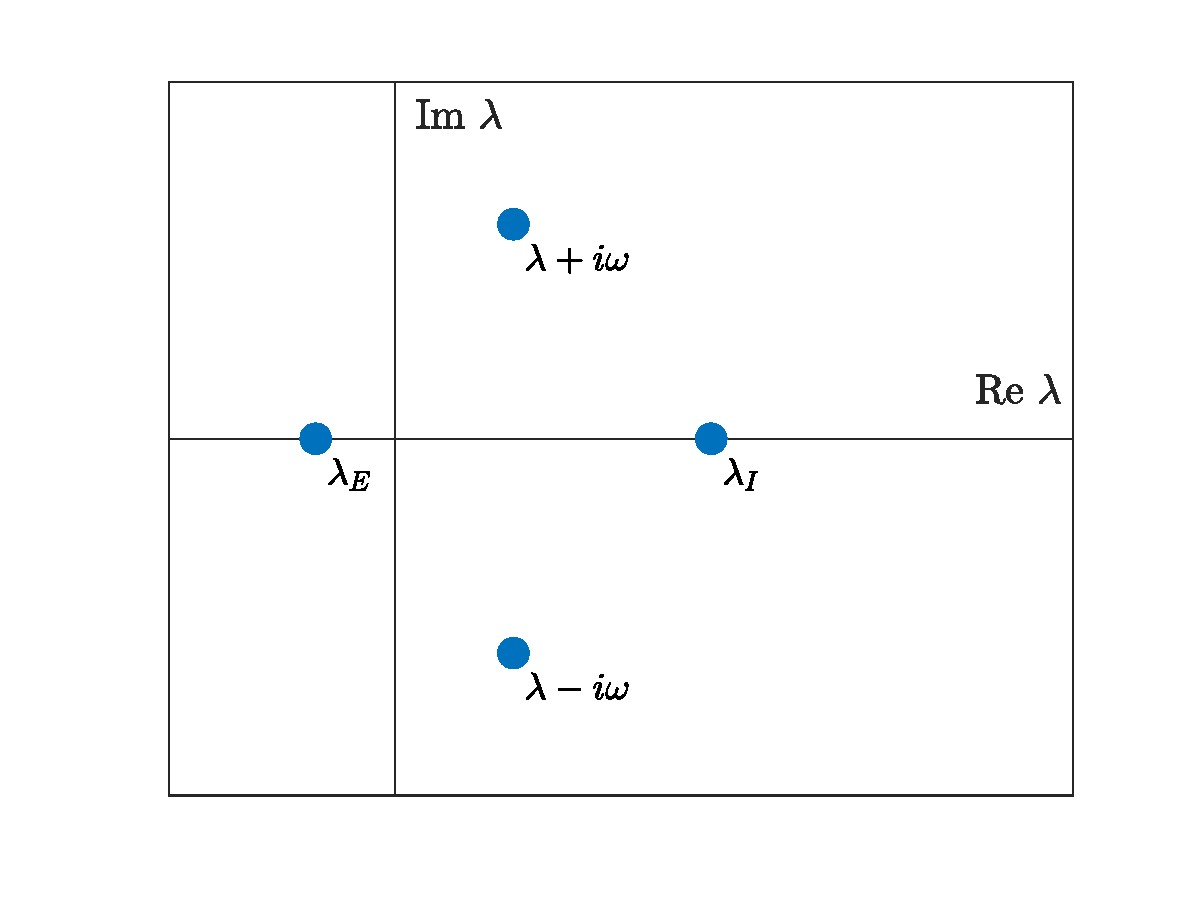
\includegraphics[width=5.7cm]{images/eigpattern1.eps} \hspace{-0.7cm}
    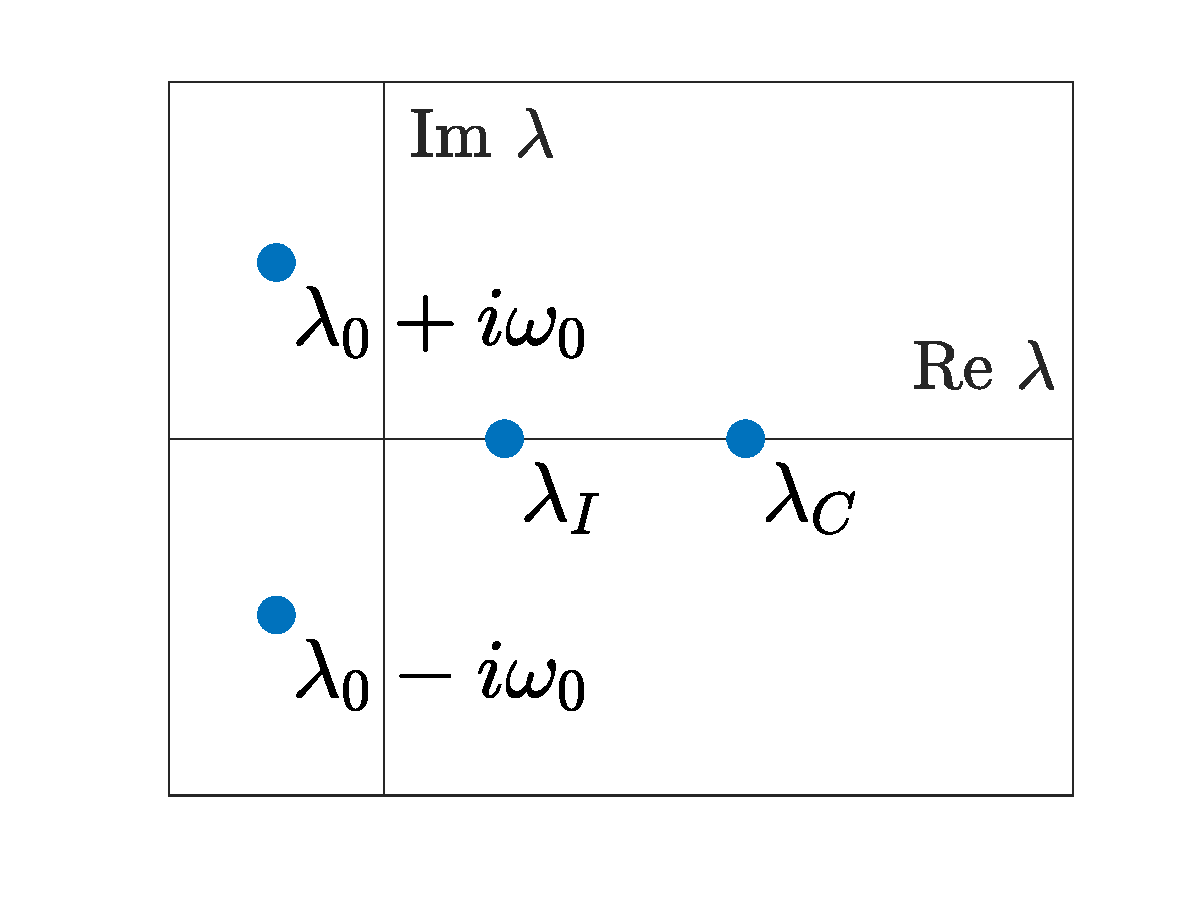
\includegraphics[width=5.7cm]{images/eigpattern2.eps} \hspace{-0.7cm}
    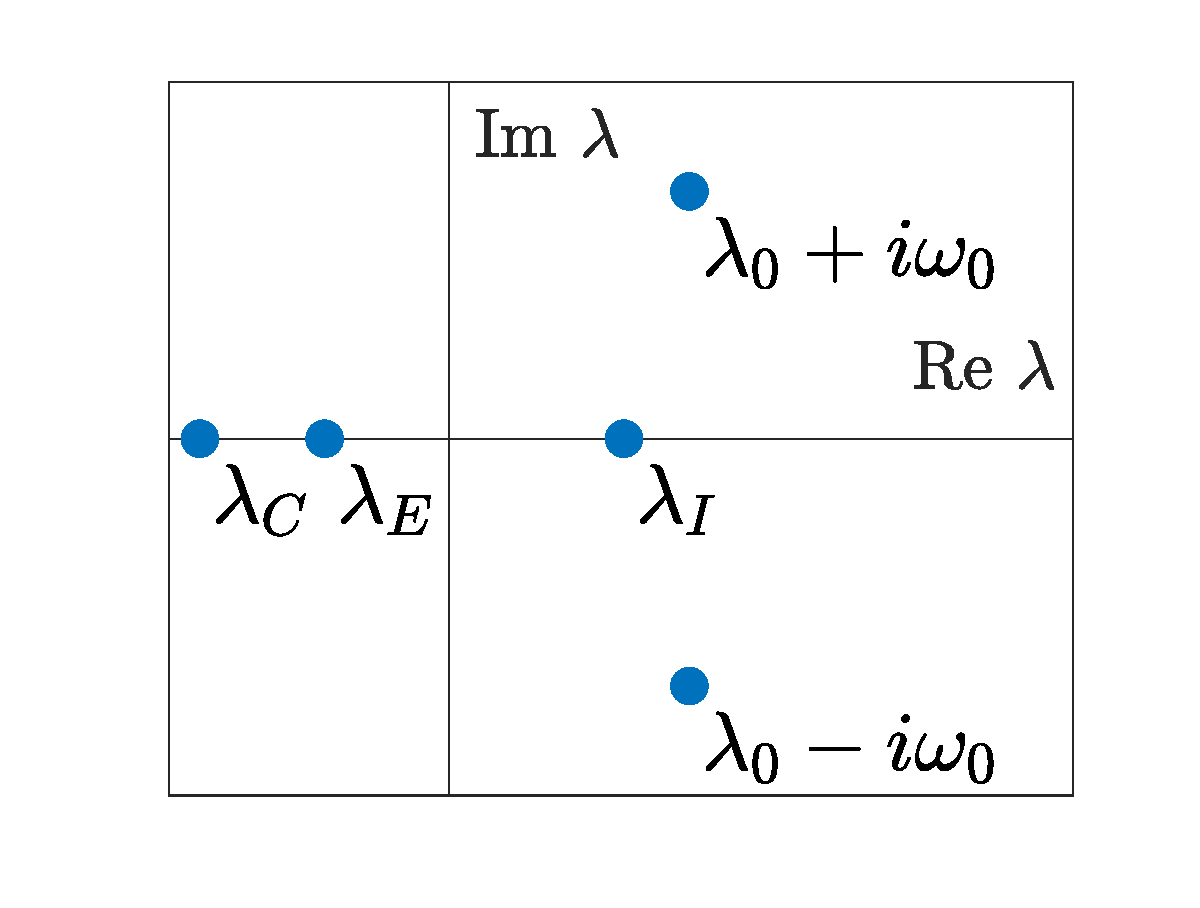
\includegraphics[width=5.7cm]{images/eigpattern3.eps} 
    % 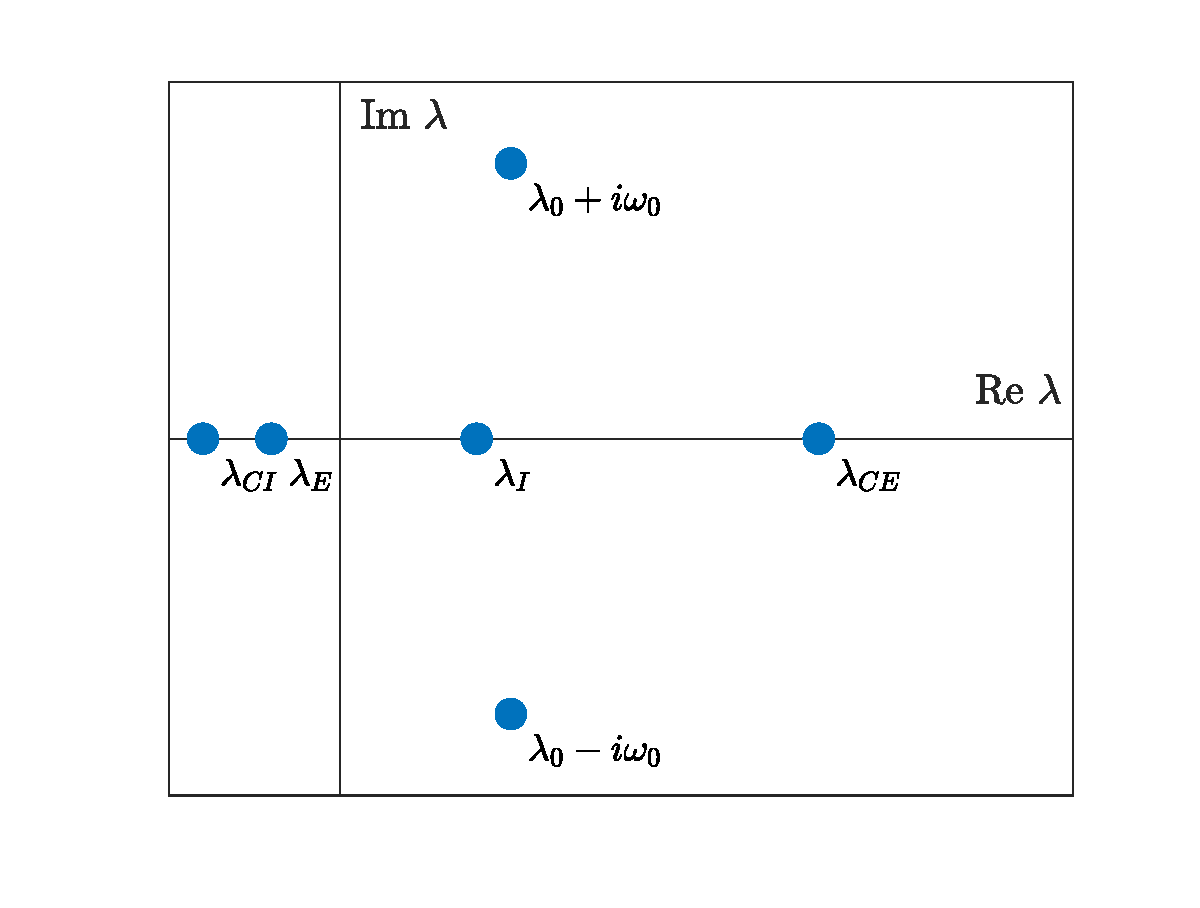
\includegraphics[width=7cm]{images/eigpattern4.eps} 
    % \end{tabular}
    \caption{Eigenvalue pattern of connectivity matrix $H$ for single excitatory and single inhibitory cluster (left), multiple excitatory clusters and single inhibitory cluster (middle), and single excitatory cluster and multiple inhibitory clusters (right). The notation for the eigenvalues in each network model is explained in the corresponding section below.}
    \label{fig:Heigpattern}
\end{figure}

\section{Model simplification}\label{sec:simplermodel}

Since our main interest is locating fixed points and periodic orbits, we can simplify the model using the fact that all excitatory cells within each excitatory cluster must be synchronized at a fixed point or periodic orbit. In the case where there is a single excitatory cluster ($n_C = 1$), if $x_1$ and $x_2$ are the activities of two excitatory cells, then it follows from \cite{Barreiro2017} that
\begin{align}\label{eq:dt_x1t2diff}
\frac{d}{dt}|x_1 - x_2|^2 \leq -2 |x_1 - x_2 |^2.
\end{align}
The only way this can be true for a fixed point (for which $\frac{d}{dt} |x_1 - x_2|^2 =0$) or for a periodic orbit (for which $x_1(t)-x_2(t) = x_1(t+T)-x_2(t+T)$ for some period $T$) is if $x_1(t) = x_2(t)$ for all $t$. If $n_C > 1$ and $x_1$ and $x_2$ are the activities of two cells in the same excitatory cluster, equation \cref{eq:dt_x1t2diff} holds by the same argument as in \cite{Barreiro2017}, since both neurons receive the same incoming connections with the same weights. 

We are primarily interested in the case where there is a single cluster of inhibitory cells ($n_{CI} = 1$). We will briefly consider the case of multiple excitatory clusters ($n_{CI} > 1$) in \cref{sec:inhibitoryclusters}. If there are $n_C$ excitatory clusters containing $p$ cells each, and $n_I$ inhibitory cells (for $N = p n_C + n_I$ total cells), equation \cref{eqn:sys_Basic} reduces to the system of $n_C + n_I$ equations
\begin{equation}\label{eq:reducedsystem}
\begin{aligned}
\dot{x}_{E_j} &= -x_{E_j} + \frac{(p-1)}{\sqrt{N}}\mu_{EE} \tanh(g x_{E_j}) + \frac{1}{\sqrt{N}} \mu_{EI} \sum_k \tanh(g x_{I_k}) && j = 1, \dots, n_C \\
\dot{x}_{I_j} &= -x_{I_j} + \frac{p}{\sqrt{N}}\mu_{IE} \sum_k \tanh(g x_{E_k}) + \frac{1}{\sqrt{N}} \mu_{II} \sum_{k\neq j}  \tanh(g x_{I_k}) && j = 1, \dots, n_I,
\end{aligned}
\end{equation}
where $x_{E_j}$ is the activity for the $j$th excitatory cluster, and $x_{I_j}$ is activity for the $j$th inhibitory cell. In matrix form, the equations \cref{eq:reducedsystem} can be written
\begin{equation}\label{eq:reducedmatrixform}
\dot{\xvec} = \tilde{F}(\xvec, g) := -\xvec + \frac{1}{\sqrt{N}} \tilde{H} \tanh(g \xvec),
\end{equation}
where $\xvec = (x_{E_1}, \dots, x_{E_{n_C}}, x_{I_1}, \dots, x_{I_{n_I}})^T$, and $\tilde{H}$ is the $(n_C + n_I) \times (n_C + n_I)$ reduced matrix
\begin{equation}\label{eq:tildeH}
\tilde{H} = \left[ \begin{array}{c|c}
    \\
    (p-1) \mu_{EE} I_{n_C} & \mu_{EI} \Onevec_{n_C \times n_I}\\
    \\
    \hline
    \\
    p \mu_{IE} \Onevec_{n_I \times n_C} & \mu_{II} \mathbf{K}_{n_I} \\
    \\
    \end{array}
    \right].
\end{equation}
Let $\xvec^* = (x_{E_1}^*, \dots, x_{E_{n_C}}^*, x_{I_1}^*, \dots, x_{I_{n_I}}^*)^T$ be a fixed point of \cref{eq:reducedmatrixform}. The linearization of \cref{eq:reducedmatrixform} about $\xvec^*$ is the matrix
\begin{equation}\label{eq:DtildeFxstar}
    D\tilde{F}(\xvec^*) = \frac{g}{\sqrt{N}}\tilde{H}(\xvec^*) - I_{n_C+n_I},
\end{equation}
where 
\begin{equation}\label{eq:tildeHxstar}
\tilde{H}(\xvec^*) := \tilde{H} \text{diag}(\sech^2(g \xvec^* )).
\end{equation}
The original equation \cref{eqn:sys_Basic} has a corresponding fixed point $\xvec_0^*$, in which each $x_{E_j}^*$ in $\xvec^*$ is repeated $p$ times. The following proposition shows that to analyze the stability of the fixed point $\xvec_0^*$ in the full system \cref{eqn:sys_Basic}, it suffices to determine the eigenvalues of the reduced matrix $\tilde{H}(\xvec^*)$.

\begin{proposition}\label{prop:tidleHeig}
Let $\xvec^*$ be a fixed point of \cref{eq:reducedmatrixform} and $\xvec_0^*$ the corresponding fixed point of \cref{eqn:sys_Basic}, and let $H(\xvec_0^*)$ and $\tilde{H}(\xvec^*)$ be defined by \cref{eq:Hxstar} and \cref{eq:tildeHxstar}. Then
\begin{compactenum}[(i)]
    \item Every eigenvalue of $\tilde{H}(\xvec^*)$ is an eigenvalue of $H(\xvec_0^*)$.
    \item $H(\xvec_0^*)$ has $n_C$ additional real, negative eigenvalues, each with multiplicity $p-1$.
\end{compactenum}
\begin{proof}
% To see this, we show that every eigenvalue of $\tilde{H}(\xvec^*)$ is also an eigenvalue of $H(\xvec_0^*)$, and that the remaining eigenvalues of $H(\xvec_0^*)$ are negative and thus will not affect stability. 
For part (i), let $\vvec = (v_{E_1}, \dots, v_{E_{n_C}}, v_{I_1}, \dots, v_{I_{n_I}})^T$ be an eigenvector of $\tilde{H}(\xvec^*)$ with eigenvalue $\lambda$. By comparing $\tilde{H}(\xvec^*)$ and $H(\xvec_0^*)$, there is a corresponding eigenvector $\vvec_0$ to $H(\xvec_0^*)$ with the same eigenvalue $\lambda$, where $\vvec_0$ is obtained from $\vvec$ by repeating each entry $v_{E_j}$ $p$ times. 
% $H(\xvec_0^*)$ has $n_E - n_C = (p-1)n_C$ additional eigenvalues which are not eigenvalues of $\tilde{H}(\xvec^*)$, which are given as follows. 
For part (ii), it can be verified directly that for $j=1, \dots, n_C$, $H(\xvec_0^*)$ has an eigenvalue at $\lambda = -\mu_{EE} \sech^2(x_{E_j})$ with multiplicity $p-1$. For $j=1$, for example, the $p-1$ eigenvectors are $\vvec^1, \dots, \vvec^{p-1}$, where $v^k_1 = -1$, $v^k_{k+1} = 1$, and all other components are 0. Since $\mu_{EE} > 0$, these eigenvalues are always negative. 
\end{proof}
\end{proposition}
 
\section{Single excitatory and inhibitory cluster}\label{sec:E1I1}

The simplest case (considered in \cite{Barreiro2017}) involves a single excitatory cluster ($n_C = 1$) and a single inhibitory cluster ($n_{CI}=1$), in which case the matrix $H$ in \cref{eqn:sys_Basic} reduces to
\[
H = 
\left[ \begin{array}{c|c}
\\
\mu_{EE} \Kvec_{n_E} & \mu_{EI} \Onevec_{n_E \times n_I}\\
\\
\hline
\\
\mu_{IE} \Onevec_{n_I \times n_E} & \mu_{II} \mathbf{K}_{n_I} \\
\\
\end{array}
\right].
\]
We choose the connection weights so that the network is \emph{balanced}; that is, the excitatory and inhibitory currents coming into each cell should approximately cancel [CITE Rajan and Abbott]. To achieve this balance, we set $\mu_{EI} = -\alpha \mu_{EE}$ and $\mu_{II} = -\alpha \mu_{IE}$, where $\alpha = \frac{f}{1-f}$. For simplicity, we also take $\mu_{IE} = \mu_{EE}$. The spectrum of $H$ is now easy to compute \cite{Barreiro2017}. The eigenvalues of $H$ (left panel of \cref{fig:Heigpattern}) are
\begin{itemize}
    \item $\lambda_I := \alpha \mu_{EE} > 0$ with multiplicity $n_I - 1$.
    \item $\lambda_E := -\mu_{EE} < 0$ with multiplicity $n_E - 1$.
    \item One complex pair of eigenvalues $\lambda_0 \pm i \omega_0$, with
    \[
    \lambda_0 := \mu_{EE}\frac{\alpha - 1}{2}, \quad \omega_0 := \mu_{EE}\sqrt{\alpha+1}\sqrt{n_E - \frac{\alpha+1}{4}}. 
    \]
\end{itemize}
It is straightforward to check that $\lambda_E < 0 < \lambda_0 < \lambda_I$. As discussed above, all bifurcations of $\xvec = 0$ involve only $\lambda_0 \pm i \omega_0$ and $\lambda_I$, which are the eigenvalues of $H$ with positive real part.

\subsection{Bifurcations of the origin}\label{sec:biforigin}

As the bifurcation parameter $g$ is increased from 0, the eigenvalue $\lambda_I^*(g)$ of $DF(0)$ corresponding to $\lambda_I$ crosses the imaginary axis at
\begin{equation}\label{eq:pitchlocation}
    g = g_0 := \frac{\sqrt{N}}{\alpha \mu_{EE}}.
\end{equation}
The origin $\xvec = 0$ is a stable equilibrium for $g < g_0$. At $g=g_0$, the origin loses stability in a symmetric pitchfork bifurcation, where $n_I - 1$ eigenvalues cross the imaginary axis simultaneously (see \cref{sec:symmpitch} below). As $g$ is further increased, the complex pair of eigenvalues $\lambda^*_0(g) \pm i \omega^*_0(g)$ of $DF(0)$ crosses the imaginary axis at 
\begin{equation}\label{eq:0hopflocation}
    g = g_H := \frac{ 2\sqrt{N} }{ (\alpha-1)\mu_{EE} },
\end{equation}
at which point a Hopf bifurcation occurs, giving rise to a limit cycle (see \cref{sec:periodic} below). The frequency of this limit cycle is given by the imaginary part $\omega^*_0(g)$ at $g = g_H$, which is
\begin{equation}\label{eq:omegag}
\omega^*_0(g_H) = \frac{2}{\alpha-1}\sqrt{\alpha+1}\sqrt{f N- \frac{\alpha+1}{4}}, 
\end{equation}
where we used $n_E = f N$. We note that since $\omega^*_0(g_H) = \mathcal{O}(\sqrt{N})$, $\omega^*_0(g_H) \rightarrow \infty$ as $N \rightarrow \infty$. 

\subsection{Solutions after symmetric pitchfork bifurcation}\label{sec:symmpitch}

Our main tool for analyzing the solutions to \cref{eqn:sys_Basic} which arise at bifurcation points when symmetries are present is the \emph{Equivariant Branching Lemma} \cite{MR631456,GSS88Vol2,HoyleRebeccaB2006Pf:a}. Before stating this result, we introduce some terminology. Let $\Gamma$ be a finite group acting on $\mathbb{R}^N$; then we say that a mapping $F: \mathbb{R}^N  \rightarrow \mathbb{R}^N$ is \emph{$\Gamma$-equivariant} if $F(\gamma \xvec) = \gamma F(\xvec)$, for all $\xvec \in \mathbb{R}^N$ and $\gamma \in \Gamma$.  A one-parameter family of mappings $F: \mathbb{R}^N \times \mathbb{R}  \rightarrow \mathbb{R}^N$ is \emph{$\Gamma$-equivariant}, if it is $\Gamma$-equivariant for each value of its second argument. We say that $V$, a subspace of $\mathbb{R}^N$, is \emph{$\Gamma$-invariant} if $\gamma \vvec \in V$, for any $\vvec$ and $\gamma \in \Gamma$. We furthermore say that the action of $\Gamma$ on $V$ is \emph{irreducible} if $V$ has no proper invariant subspaces, i.e. the only $\Gamma$-invariant subspaces of $V$ are $\{0\}$ and $V$ itself. 

For a group $\Gamma$ and a vector space $V$, we define the \emph{fixed-point subspace} for $\Gamma$, denoted $\rm{Fix} (\Gamma)$, to be all points in $V$ that are unchanged under any of the members of $\Gamma$, i.e. $\rm{Fix} (\Gamma) = \{ \xvec \in V : \gamma \xvec = \xvec, \forall \gamma \in \Gamma \}$. 
%\Acomment{Note that isotropy subgroup has two meanings: check that I am correct about this} 
The \textit{isotropy subgroup of $\xvec \in V$}, denoted $\Sigma_x$, is the set of all members of $\Gamma$ under which $\xvec$ is fixed, i.e. $\Sigma_x = \{ \gamma \in \Gamma : \gamma \xvec = \xvec \}$. We then say that a subgroup $\Sigma$ is \textit{an} isotropy subgroup of $\Gamma$, if it is the isotropy subgroup, $\Sigma_x$, for some $\xvec \in V$.

Suppose we have a one-parameter family of mappings, $F(\xvec, g)$, and we wish to solve $F(\xvec, g)=0$. 
For any $(\xvec, g) \in \mathbb{R}^n \times \mathbb{R}$, let $(dF)_{\xvec,g}$ denote the $N \times N$ Jacobian matrix 
\[ \left[ \frac{\partial F_j}{\partial x_k} (\xvec, g) \right]_{j, k=1...N}
\] 
A bifurcation will occur when the Jacobian ceases to be invertible, i.e. when $(dF)_{\xvec,g}$ has a nontrivial kernel. For a $\Gamma$-equivariant mapping --- i.e. $F(\xvec,g)$ is $\Gamma$-equivariant for any value of the parameter $g$ --- we may have \textit{multiple} eigenvalues go through zero at once, because of symmetries; however, the structural changes that occur are qualitatively the same as those that occur in a non-symmetric system in which a single eigenvalue crosses through zero. Furthermore, we will have \emph{multiple} such solution branches, each corresponding to a subgroup of the original symmetries, which is formalized in the following theorem:

%Then the Implicit Function Theorem states that we can continue to track a unique solution branch as a function of $g$, as long as the Jacobian remains invertible. When this ceases to be true --- when $(dF)_{\xvec,g}$ has a nontrivial kernel --- we have the possibility for a bifurcation. At this point the number of zero eigenvalues (whether there are one, or two, etc..) and a menagerie of further conditions will determine the qualitative properties of the structural change that occurs.
%that is $\rm{det} dF \not= 0$, where $dF_{jk} = \left( \frac{\partial F_j}{\partial x_k} \right)  It states conditions for 

%What complicates this situation for $\Gamma$-equivariant mappings --- i.e. $F(\xvec,g)$ is $\Gamma$-equivariant for any value of the parameter $g$ --- is that because of symmetries, \textit{multiple} eigenvalues will go through zero at once; however, the structural changes that occur are qualitatively the same as those that occur in a non-symmetric system, with a single zero eigenvalue. What changes is that we now have \textit{multiple} such solution branches, each corresponding to a subgroup of the original symmetries.  The following Lemma formalizes this fact:\\


\begin{theorem}[Equivariant Branching Lemma: paraphrased from \cite{GSS88Vol2}, pg. 82, see also pg. 67-69] Let $F: \mathbb{R}^N \times \mathbb{R} \rightarrow \mathbb{R}^N$ be a one-parameter family of $\Gamma$-equivariant mappings with $F(\xvec_0, g_0) = \Zerovec$. Suppose that $(\xvec_0, g_0)$ is a bifurcation point and that, defining $V = \ker(dF)_{\xvec_0, g_0}$, $\Gamma$ acts absolutely irreducibly on $V$. Let $\Sigma$ be an isotropy subgroup of $\Gamma$ satisfying 
\begin{eqnarray}
\rm{dim}\; \rm{Fix} (\Sigma) = 1,
\end{eqnarray}
where $\rm{Fix (\Sigma)}$ is the \emph{fixed-point subspace} of $\Sigma$: that is, $\rm{Fix} (\Sigma) \equiv \{ x \in V \mid \sigma x = x, \;  \forall \sigma \in \Sigma \}$. Then there exists a unique smooth solution branch to $F = 0$ such that the isotropy subgroup of each solution is $\Sigma$.
\end{theorem}

The reader can readily check that the right-hand side of \cref{eqn:sys_Basic} is $\Gamma$-equivariant, for $\Gamma = S_{n_E} \times S_{n_I}$, where $S_n$ is the group of permutations on $n$ objects. That is, we can permute the labels on the excitatory cells, and/or the labels on the inhibitory cells, without changing the equations.

At $g=g_0$, $n_I -1$ eigenvalues pass through zero: the corresponding eigenspace is the set of all zero-sum vectors with support in the inhibitory cells only; i.e. 
\[ V \equiv  \ker(dF)_{\Zerovec,g^{\ast}}  = {\rm span} \, \left\{ \left[  
\underbrace{\begin{matrix}0 & \cdots & 0\end{matrix}}_{n_{E}} \;
\vvec_{n_{I}} \right] \right\}, \qquad \vvec_{n_{I}} \perp \Onevec_{n_{I}}.
\]
To check that $\Gamma$ acts irreducibly on $V$ it is sufficient to show that the subspace spanned by the \textit{orbit} of a single vector $\vvec$ (defined as the set of all values  $\gamma \vvec$, for $\gamma \in \Gamma$) is full rank; this can be readily confirmed for $\vvec_{n_{I}} = \left[ \begin{array}{ccccc} 1 & -1 & 0 & ... & 0 \end{array} \right]$, for example.   

To find the appropriate subgroup of symmetries, we break the inhibitory cells up into precisely two clusters and retain only permutations within each cluster. This describes a subgroup of $\Gamma$, $\Sigma = S_{n_E} \times S_{n_{I_1}} \times S_{n_{I_2}}$, $n_{I_1} + n_{I_2} = n_I$.
Assuming that (without loss of generality) the $I_1$ neurons have the indices $n_E+1,...,n_E+n_{I_1}$, and so forth, $\Sigma$ has the fixed point subspace 
\begin{eqnarray}
\rm{Fix}(\Sigma) & = & {\rm span} \, \left\{ \left[  
\underbrace{\begin{matrix}0 & \cdots & 0\end{matrix}}_{n_E} \;
\underbrace{\begin{matrix}1 & \cdots & 1\end{matrix}}_{n_{I_1}} \;
\underbrace{\begin{matrix}-\frac{n_{I_1}}{n_{I_2}} & \cdots & -\frac{n_{I_1}}{n_{I_2}} \end{matrix}}_{n_{I_2}} \right] \right\}.
\end{eqnarray}
We can check that $\rm{Fix}(\Sigma)$ is a subspace of $V$. Furthermore $\dim \rm{Fix}(\Sigma) = 1$ because it can be described as the span of a single vector. 

As a consequence, there is a branch of equilibria emerging at the symmetric pitchfork bifurcation point $g=g_0$ for every possible division of the inhibitory cells into exactly two clusters of size $n_{I_1}$ and $n_{I_2}$, where $n_{I_1} + n_{I_2} = n_I$. We refer to these as $I_1/I_2$ branches.  Each such branch may be characterized by the number $\beta = n_{I_1}/n_{I_2}$, which gives the ratio of the cluster sizes. Without loss of generality, we may take $n_{I_1} \geq n_{I_2}$, so that $\beta \geq 1$. The inhibitory cells within each of the two clusters are synchronized. The solution on each $I_1/I_2$ branch is then given as $(x_E, x_{I_1}, x_{I_2})$. Due to the odd symmetry of \cref{eqn:sys_Basic}, there is a corresponding $I_1/I_2$ branch for each $\beta$ with solution $(-x_E, -x_{I_1}, -x_{I_2})$, which we will ignore for simplicity.

\subsection{Solutions along \texorpdfstring{$I_1/I_2$}{I1/I2} branches}

First, we derive leading order expressions for the equilibria along the $I_1/I_2$ branches for $g$ close to $g_0$. Recall from \cref{sec:simplermodel} that we only need to solve \cref{eq:reducedsystem} since all excitatory cells are synchronized. 

The simplest case occurs when $n_I$ is even and $\beta = 1$, in which case $n_{I_1}=n_{I_2}$. On this branch, $x_E = 0$, and $x_{I_2} = -x_{I_1}$, i.e. there are two equally sized inhibitory populations with equal and opposite activities, and there is no excitatory cell activity. Beginning with the single remaining equation for $x_{I_1}$, and utilizing the Taylor expansion for the $\tanh$ function, we show (see detailed calculations in Appendix) that 
the nonzero solution for $x_I$ is given, to leading order, by
\begin{align}\label{eq:xIapprox}
x_I &= \sqrt{ \frac{3(g - g_0) }{g^3}} && g \geq g_0.
\end{align}

We can obtain a higher-order approximation by keeping up to fifth-order terms in \cref{eq:tanhTaylor} to get
\begin{equation*}
x_I \left( (g - g_0) - \frac{g^3}{3} x_I^2 + \frac{2 g^5}{15} x_I^4 \right) = 0,
\end{equation*}
which is $x_I$ multiplied by a quadratic in $x_I^2$. To find the nonzero solution for $x_I$, we solve this quadratic for $x_I^2$ and take square roots to get, to leading order,
\begin{align}\label{eq:xIapprox5}
x_I &= \frac{1}{2} \sqrt{ \frac{5}{g^2} - \frac{\sqrt{ 5 g^5( 24 g_0 - 19 g) }}{g^5}} && g \geq g_0.
\end{align}
Comparison between the third-order approximation \cref{eq:xIapprox}, the fifth-order approximation \cref{eq:xIapprox5}, and the numerical solution obtained by parameter continuation is shown in the left panel of \cref{fig:xIapprox}.

\begin{figure}
    \centering
    \begin{tabular}{cc}
    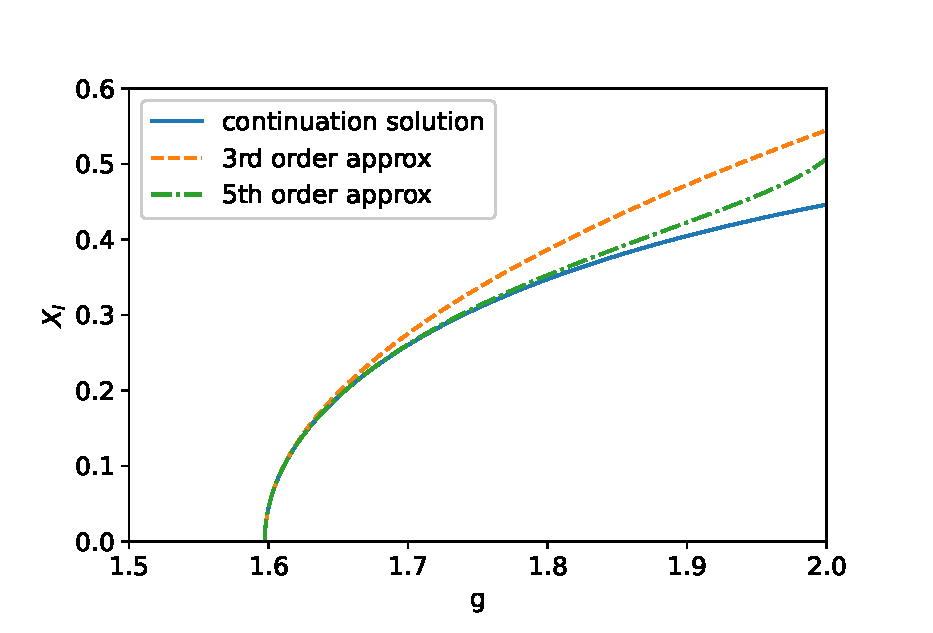
\includegraphics[width=7.8cm]{images/Xiapprox.eps} &
    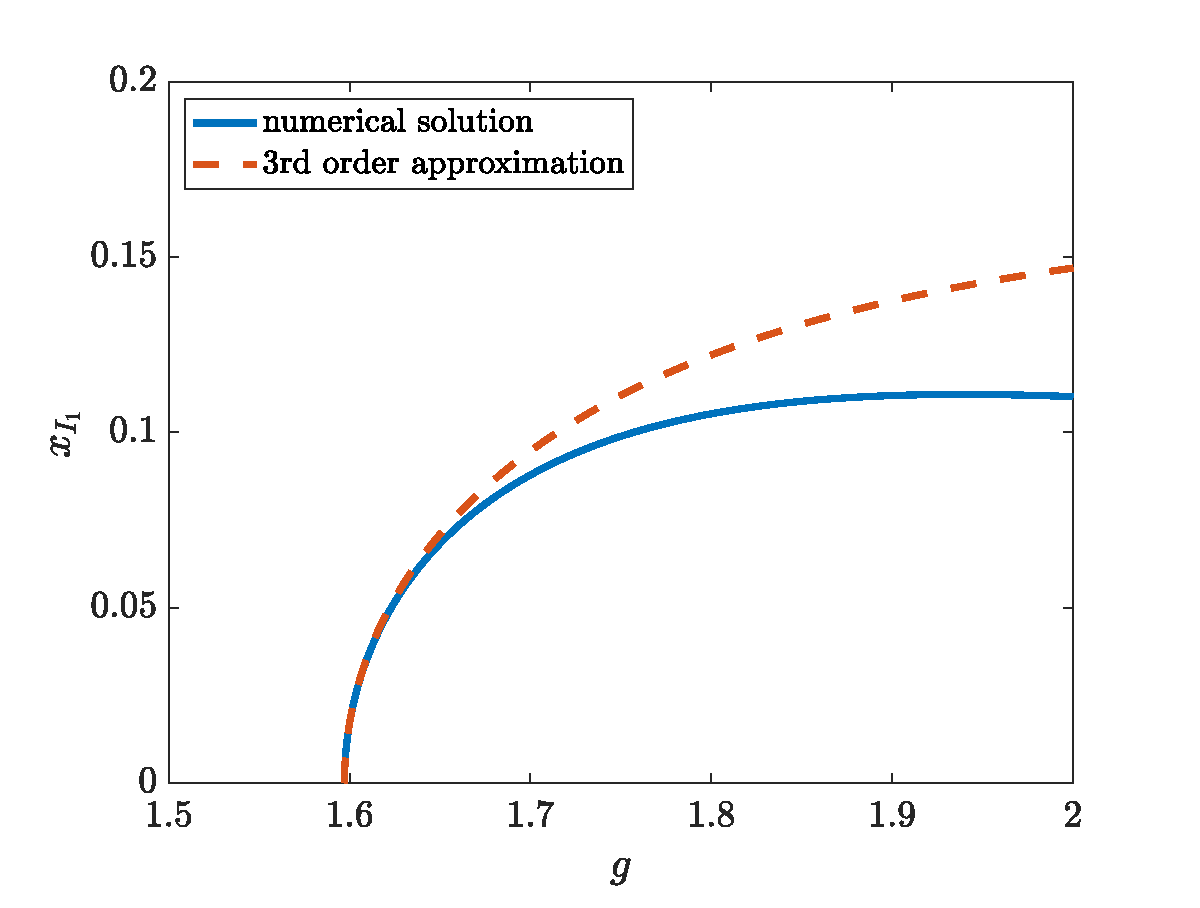
\includegraphics[width=7.8cm]{images/Xiapproxbeta3.eps} 
    \end{tabular}
    \caption{Third order approximation \cref{eq:xIapprox} and fifth order approximation \cref{eq:xIapprox5} to $x_I$ on the $I_1=I_2$ branch of fixed points (left panel). Third order approximation \cref{eq:XI1} to $X_{I_1}$ on the $\beta=3$ branch (right panel). $N = 20$,  $\alpha = 4$, $\mu_{EE} = 0.7$.}
    \label{fig:xIapprox}
\end{figure}

For $\beta > 1$, it is no longer true that $x_{I_2} = -x_{I_1}$. However, by making an appropriate ansatz and proceding as described in the Appendix (), 
we obtain an approximate formula for $x_{I_1}$ in terms of $g$, for $g$ close to $g_0$
 \begin{align}\label{eq:XI1}
 x_{I_1} &= \sqrt{ \frac{ 3(g - g_0) }{ (1 - \beta + \beta^2 )g^3}} + \mathcal{O}\left( \frac{1}{N^2}\right)&& g \geq g_0.
\end{align}
Note that this reduces to \cref{eq:xIapprox} when $\beta = 1$. Comparison between this approximation and the numerical solution obtained by numerical parameter continuation is shown in the right panel of \cref{fig:xIapprox}.

\begin{figure}
    \centering
    \begin{tabular}{cc}
    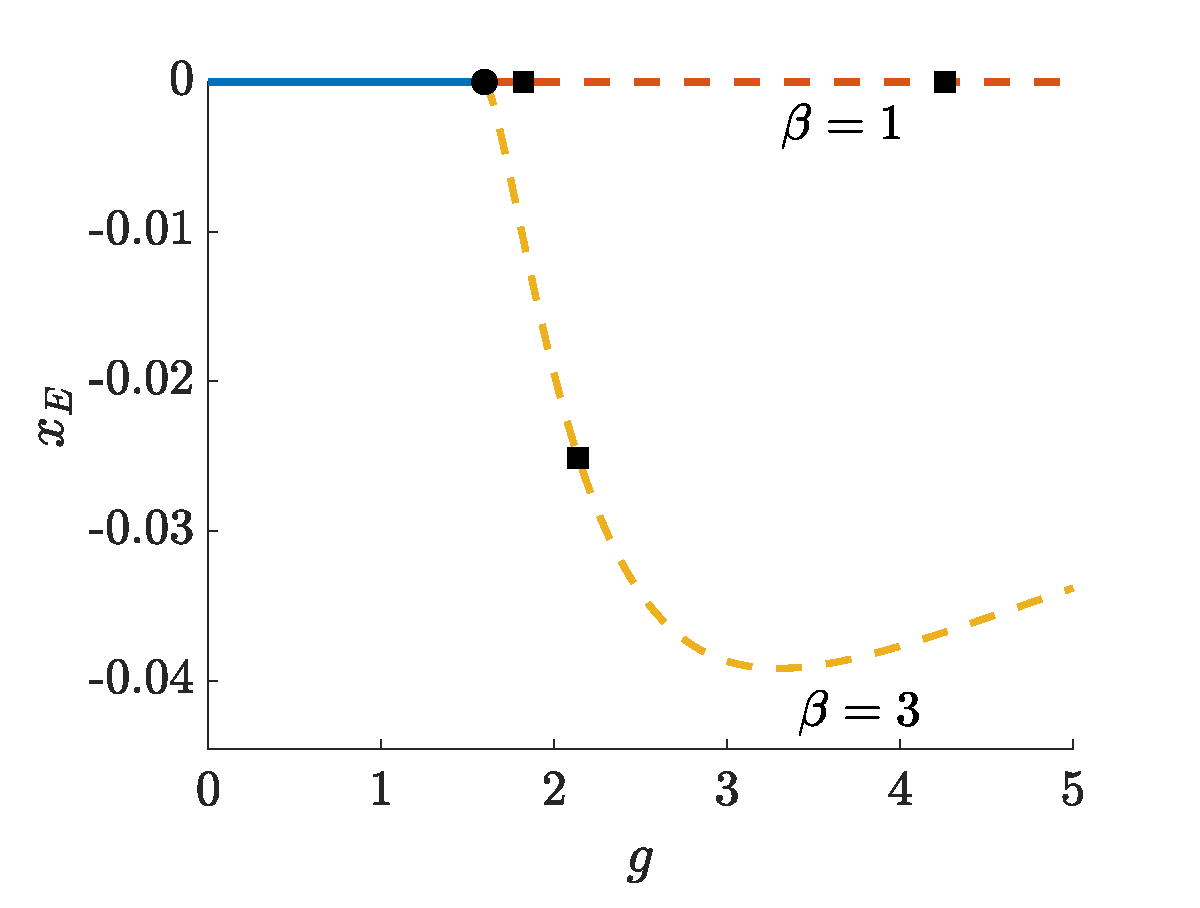
\includegraphics[width=7.8cm]{images/bdnoclusters20E.eps} &
    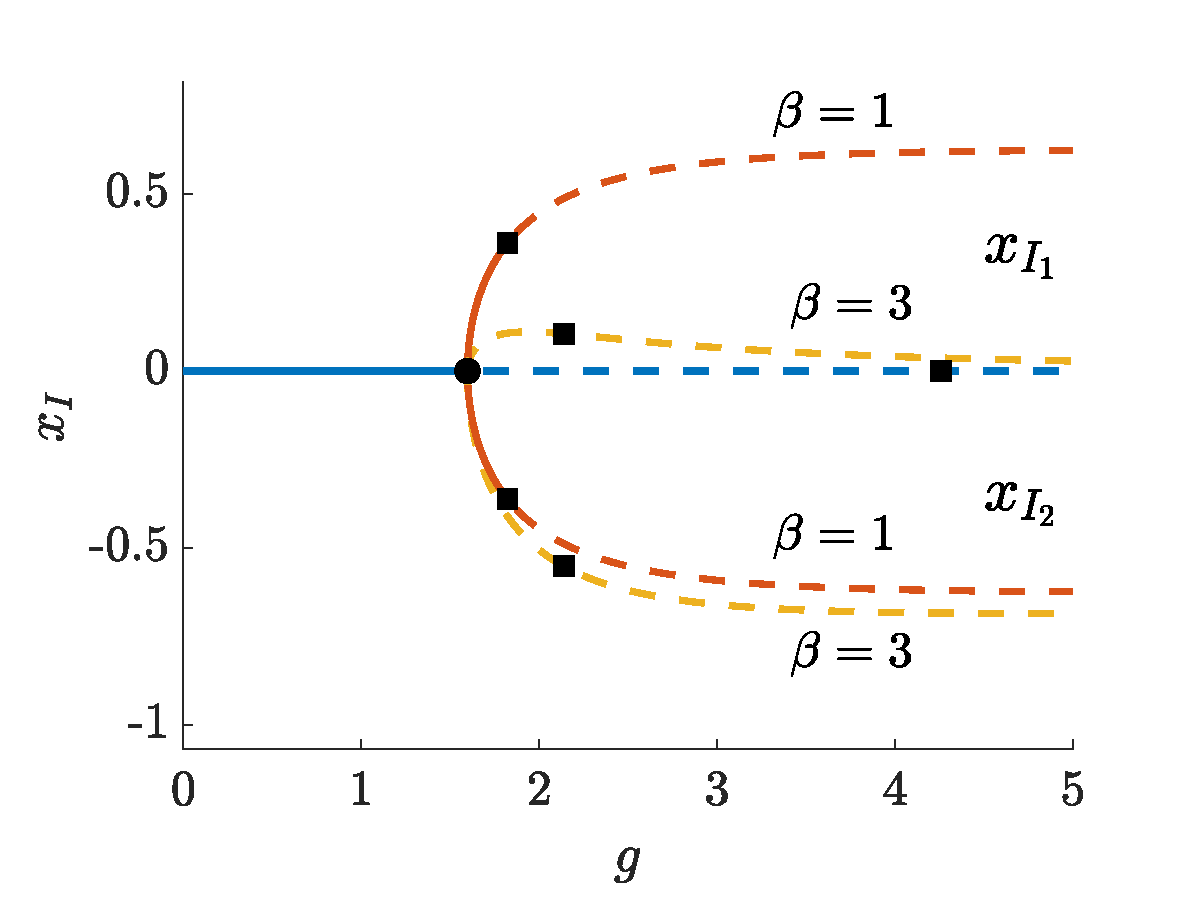
\includegraphics[width=7.8cm]{images/bdnoclusters20I.eps} \\
    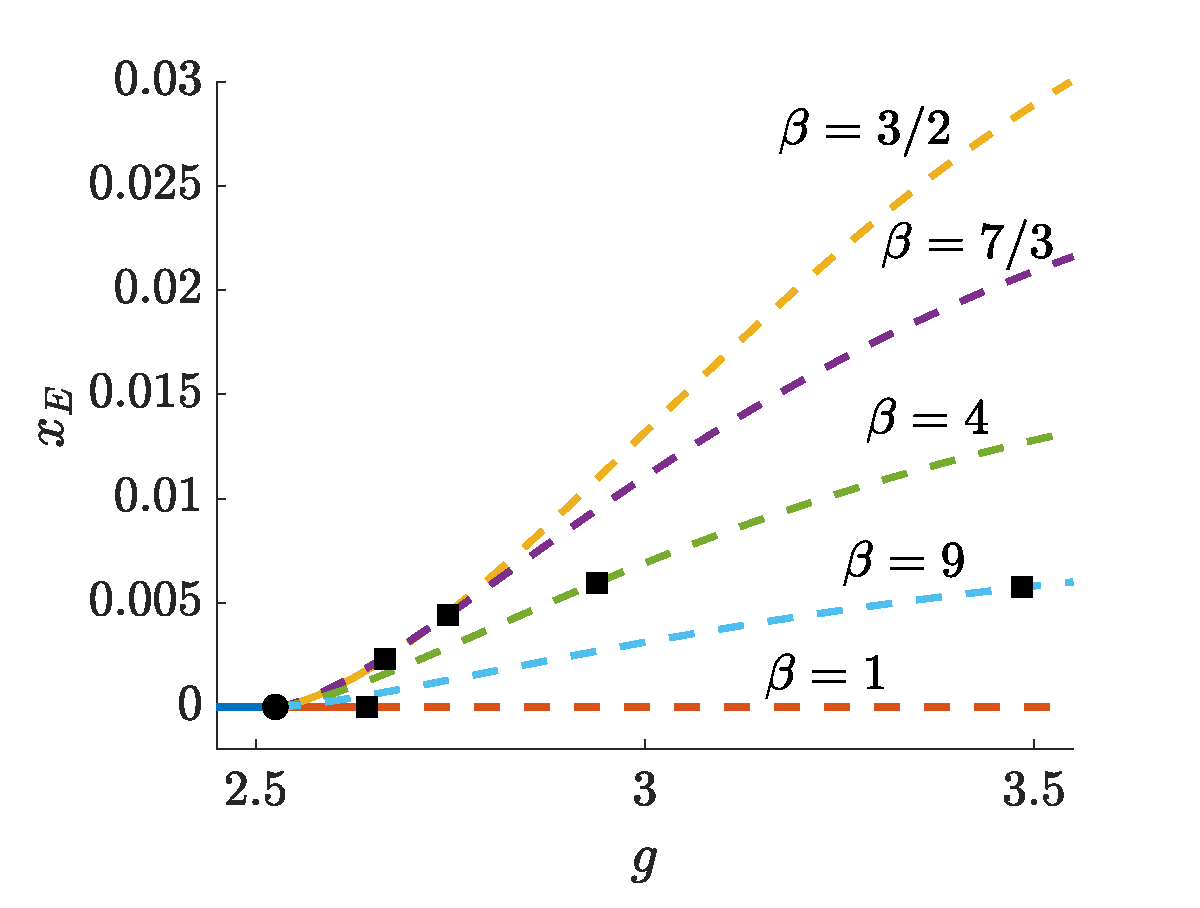
\includegraphics[width=7.8cm]{images/bdnoclusters50E.eps} &
    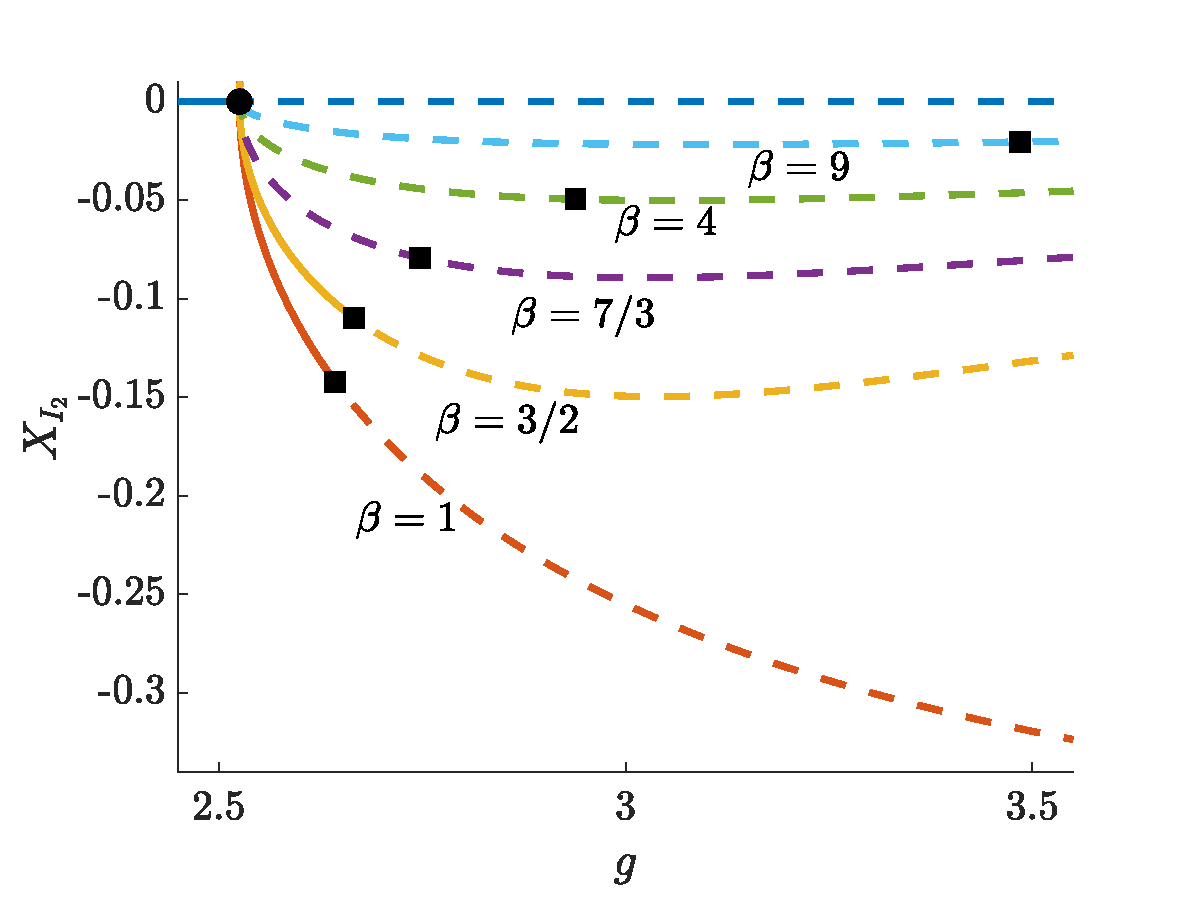
\includegraphics[width=7.8cm]{images/bdnoclusters50I.eps}
    \end{tabular}
    \caption{Bifurcation diagram showing $I_1/I_2$ branches of equilibria of \cref{eqn:sys_Basic} for all valid values of $\beta$. Top panels show $N=20$, with top left plotting $X_E$ vs $g$, and top right plotting $X_{I_1}$ (above horizontal axis) and $X_{I_2}$ (below horizontal axis) vs $g$. Bottom panels show $N=50$, with bottom left plotting $X_E$ vs $g$, and bottom right plotting $X_{I_2}$ only vs $g$. Solid lines indicate stable fixed points, dashed lines indicate unstable fixed points. Symmetric pitchfork bifurcation at $g = g_0$ indicated with filled circle. Hopf bifurcations indicated with filled squares. Further bifurcations along branches are not shown to avoid clutter. $\alpha = 4$, $\mu_{EE} = 0.7$.}
    \label{fig:noclusterBD1}
\end{figure}

\subsection{Stability and bifurcations along \texorpdfstring{$I_1/I_2$}{I1/I2} branches}

Now that we have obtained a leading order formula for the fixed points on the $I_1/I_2$ branches for all valid inhibitory cell ratios $\beta$, we will analyze their stability for $g$ close to the bifurcation point $g_0$. Choose any $\beta \geq 1$, so that $n_{I_1} = \frac{\beta}{\beta+1}n_I$ and $n_{I_2} = \frac{1}{\beta+1}n_I$, and let $\xvec = (x_E, x_{I_1}, x_{I_2})$ be a solution to \cref{eq:otherbranchmatrixeq} for $g > g_0$. To examine the stability and bifurcations which occur along the $I_1/I_2$ branches, we look at the linearization $D\tilde{F}(\xvec^*)$, where $\xvec^* = (x_E, x_{I_1}, \dots, x_{I_1}, x_{I_2}, \dots, x_{I_2})^T$, and $x_{I_1}$ and $x_{I_2}$ are repeated $n_{I_1}$ and $n_{I_2}$ times, respectively. As discussed above in \cref{sec:simplermodel}, stability will depend on the eigenvalues of $\tilde{H}(\xvec^*)$. A cartoon showing the location of these eigenvalues is given in \cref{fig:Hstareignocluster}. In the process of our analysis, we will show that a Hopf bifurcation occurs along each $I_1/I_2$ branch, and will find a leading order formula for its location.

\begin{figure}
    \centering
    % \begin{tabular}{ccc}
    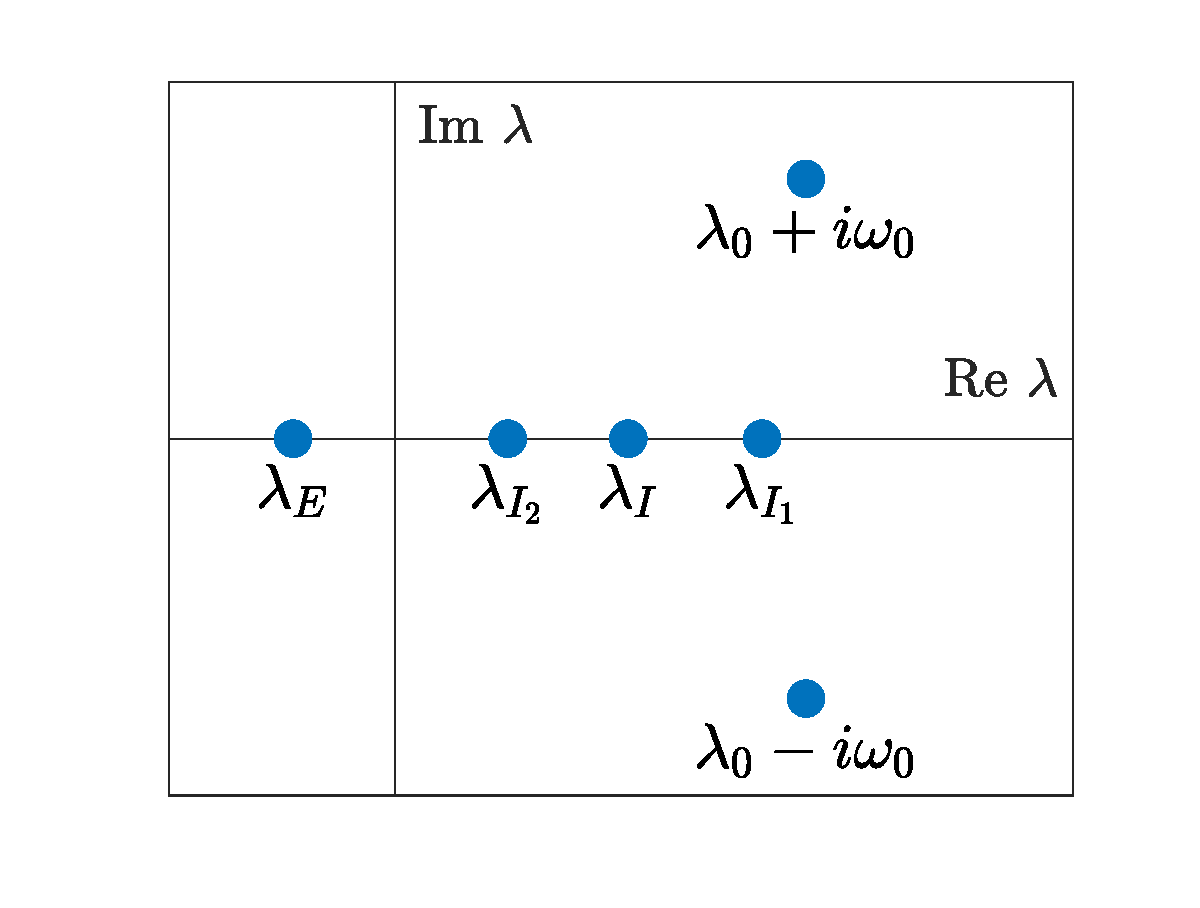
\includegraphics[width=5.7cm]{images/eigpatternxstarnocluster.eps}
    % \end{tabular}
    \caption{Eigenvalue pattern of connectivity matrix $H(\xvec^*)$ for fixed point $\xvec^*$ on $I_1/I_2$ branch with $\beta > 1$. The notation for the eigenvalues is explained below.}
    \label{fig:Hstareignocluster}
\end{figure}

To locate the eigenvalues of $\tilde{H}(\xvec^*)$, we first linearize the three-dimensional system \cref{eq:otherbranchmatrixeq} about the fixed point $\xvec = (x_E, x_{I_1}, x_{I_2})$ to get the Jacobian
\[
J_3(\xvec) = \frac{g}{\sqrt{N}} H_3(\xvec) - I_3
\]
where 
\begin{equation}\label{eq:H3}
H_3(\xvec) = \mu_{EE}
 \begin{bmatrix} (\alpha n_I - 1) \sech^2(g x_E) & -\alpha \frac{\beta}{\beta+1} n_I \sech^2(g x_{I_1}) & - \alpha \frac{1}{\beta+1} n_I \sech^2(g x_{I_2}) \\
    \alpha n_I \sech^2(g x_E) & -\alpha \left(\frac{\beta}{\beta+1} n_I-1\right) \sech^2(g x_{I_1}) & -\alpha \frac{1}{\beta+1} n_I \sech^2(g x_{I_2}) \\
    \alpha n_I \sech^2(g x_E) & -\alpha \frac{\beta}{\beta+1} n_I \sech^2(g x_{I_1}) & -\alpha \left(\frac{1}{\beta+1} n_I-1 \right) \sech^2(g x_{I_2})
 \end{bmatrix}
\end{equation}
% \[
% H_3(\xvec) = \mu_{EE} 
%  \begin{bmatrix} (\alpha n_I - 1) & -\alpha \frac{\beta}{\beta+1} n_I & - \alpha \frac{1}{\beta+1} n_I \\
%     \alpha n_I  & -\alpha \left(\frac{\beta}{\beta+1} n_I-1\right) & -\alpha \frac{1}{\beta+1} n_I \\
%     \alpha n_I & -\alpha \frac{\beta}{\beta+1} n_I & -\alpha \left(\frac{1}{\beta+1} n_I-1 \right) 
%  \end{bmatrix}
%  \begin{bmatrix} \sech^2(g x_E) & 0 & 0 \\0 & \sech^2(g x_{I_1}) & 0\\0 & 0 & \sech^2(g x_{I_2}) \end{bmatrix} 
% \]
and $I_3$ is the $3 \times 3$ identity matrix. We have the following proposition concerning the eigenvalues of $H_3(\xvec)$ and $\tilde{H}(\xvec^*)$.

\begin{proposition}\label{prop:H3eig}
Let $\xvec = (x_E, x_{I_1}, x_{I_2})$ be a solution of \cref{eq:otherbranchmatrixeq} and $\xvec^*$ the corresponding fixed point of \cref{eq:reducedmatrixform}, and let $H_3(\xvec)$ and $\tilde{H}(\xvec^*)$ be defined by \cref{eq:H3} and \cref{eq:tildeHxstar}. Then
\begin{compactenum}[(i)]
    \item Every eigenvalue of $H_3(\xvec)$ is an eigenvalue of $\tilde{H}(\xvec^*)$.
    \item $\tilde{H}(\xvec^*)$ has the following additional eigenvalues:
    \begin{itemize}
        \item $\lambda_{I_1} := \mu_{EE} \alpha \sech^2(g x_{I_1})$ with multiplicity $n_{I_1}-1$.
        \item $\lambda_{I_2} := \mu_{EE} \alpha \sech^2(g x_{I_2})$ with multiplicity $n_{I_2}-1$
    \end{itemize}
\end{compactenum}
\begin{proof}
For part (i), if $\lambda$ is an eigenvalue of $H_3(\xvec)$ with eigenvector $\vvec = (v_E, v_{I_1}, v_{I_2})$, then $\lambda$ is also an eigenvalue of $\tilde{H}(\xvec^*)$ with eigenvector $\vvec = (v_E, v_{I_1}, \dots, v_{I_1}, v_{I_2}, \dots, v_{I_2})$, where $v_{I_1}$ and $v_{I_2}$ are repeated $n_{I_1}$ and $n_{I_2}$ times. For part (ii), if $n_{I_1} > 1$, then it can be verified directly that $\tilde{H}(\xvec^*)$ has an eigenvalue $\lambda_{I_1} = \mu_{EE} \alpha \sech^2(g x_{I_1})$ with multiplicity $n_{I_1}-1$. The corresponding eigenvectors are $\vvec^1, \dots, \vvec^{n_{I_1}-1}$, where $v^k_2 = -1$, $v^k_{k+2} = 1$, and all other components are 0. If $n_{I_2} > 1$, the eigenvalue $\lambda_{I_2}$ can be similarly obtained.
\end{proof}
\end{proposition}

To determine the stability of $\xvec^*$ for $g$ close to $g_0$, we must compute the eigenvalues of $D\tilde{F}(\xvec^*)$ corresponding to $\lambda_{I_1}$ and $\lambda_{I_2}$. We will find (see Appendix) that $\lambda_{I_2}$ is always negative, while $\lambda_{I_1}$ is negative for $\beta<2$ and positive otherwise. Therefore the fixed point is unstable for $\beta \ge 2$ (see \cref{fig:noclusterBD1}). 

The eigenvalues of $H_3$ include one real eigenvalue and a complex pair; the real eigenvalue is always negative, and the complex pair crosses the real axis at a Hopf bifurcation. We find that its location is

% If $\beta = 1$, $x_{I_2} = -x_{I_1} := x_I$, thus $\tilde{H}(\xvec^*)$ has a single additional eigenvalue $\lambda_{I} := \mu_{EE} \alpha \sech^2(g x_{I})$ with multiplicity $n_I - 2$. The corresponding eigenvalue of $D\tilde{F}(\xvec^*)$ is $\lambda_{I}^* = -2\left( \frac{g - g_0}{g_0} \right)$, which is negative for $g > g_0$.

\begin{equation}\label{eq:ghopfformula}
    g_{H,\beta} = 
    \frac{\sqrt{N}}{\mu_{EE}} 
    \frac{ 2 - 5\beta + 2 \beta^2 + 3 \beta n_I}
    { \alpha(1 - 4 \beta + \beta^2) - (1 - \beta + \beta^2) + 3 \alpha \beta n_I }
    + \mathcal{O}\left( \frac{1}{N^{3/2}} \right).
\end{equation}
A plot of $g_{H,\beta}$ versus $N$ for various $\beta$ is given in \cref{fig:Hopfplots}. We note that a Hopf bifurcation for a particular value of $\beta$ will only occur in a real network if the ratio of inhibitory cells is valid for that particular value of $N$ (e.g. for $\beta = 3$, the total number of inhibitory cells must be a multiple of 4). The leading order term of \cref{eq:ghopfformula}, as well as the order of the remainder term, agrees with results from numerical parameter continuation (\cref{fig:Hopfplots}). As $N \rightarrow \infty$, which implies $n_I = f N \rightarrow \infty$, the first terms in the numerator and denominator of \cref{eq:ghopfformula} dominate, thus $g_{H,\beta} \rightarrow g_0$ as $N \rightarrow \infty$ for all $\beta$ (see \cref{fig:Hopfplots}). Differentiating the leading order term in \cref{eq:ghopfformula} with respect to $\beta$ and simplifying,
\begin{equation}\label{eq:gprime}
g_{H,\beta}' = \frac{ \sqrt{N} }{ \mu_{EE} }
    \frac{ 
    3(\alpha+1)(\beta^2-1)(n_I-1)
    }
    { 
        \left[ \alpha(1 - 4 \beta + \beta^2) - (1 - \beta + \beta^2) + 3 \alpha \beta n_I \right]^2
    }\:,
\end{equation}
which is 0 at $\beta = 1$ and positive for $\beta > 1$. As a consequence, $g_{H,\beta}$ increases with $\beta$ for $\beta \geq 1$ (see \cref{fig:Hopfplots} for this ordering in $\beta$, as well as \cref{fig:noclusterBD1}). 

\begin{figure}
    \centering
    \begin{tabular}{cc}
    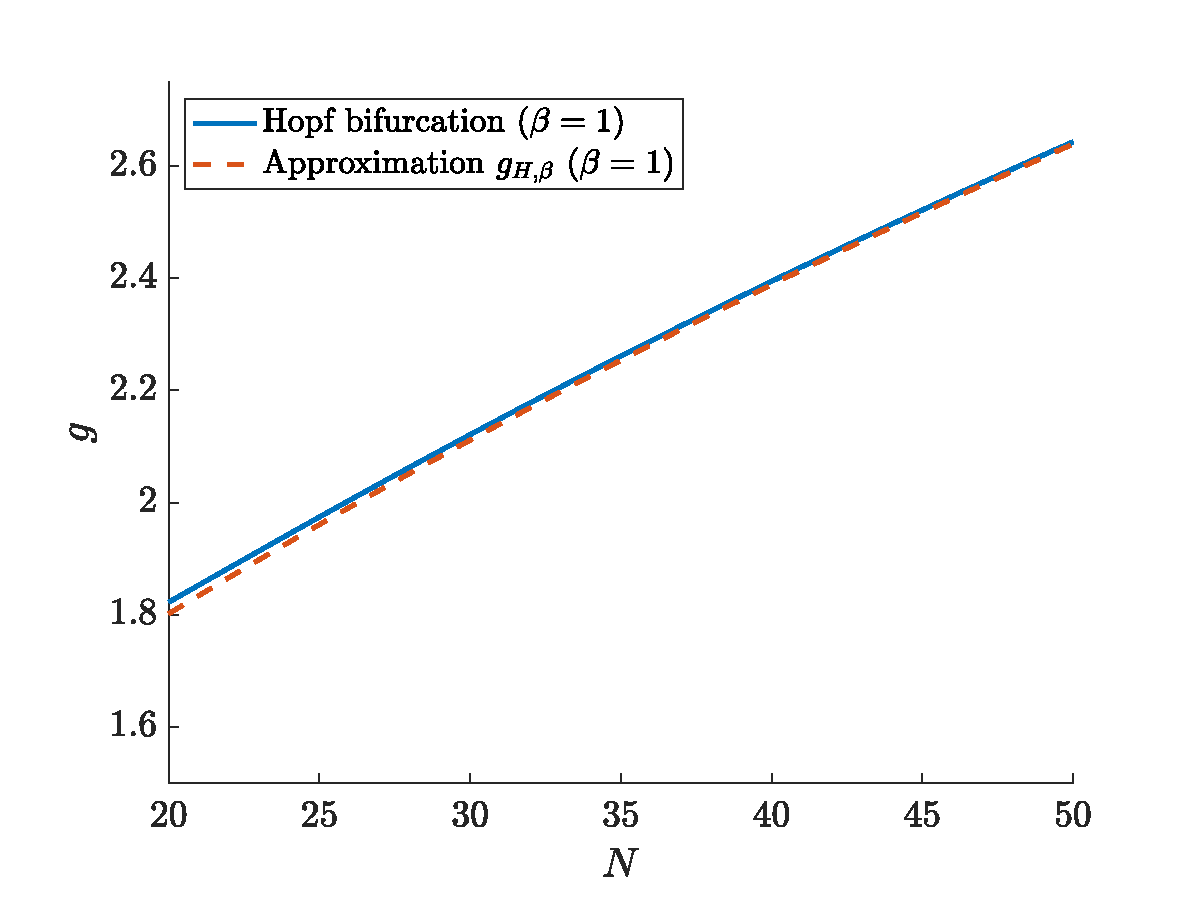
\includegraphics[width=7.8cm]{images/Hopfapproxbeta1.eps} &
    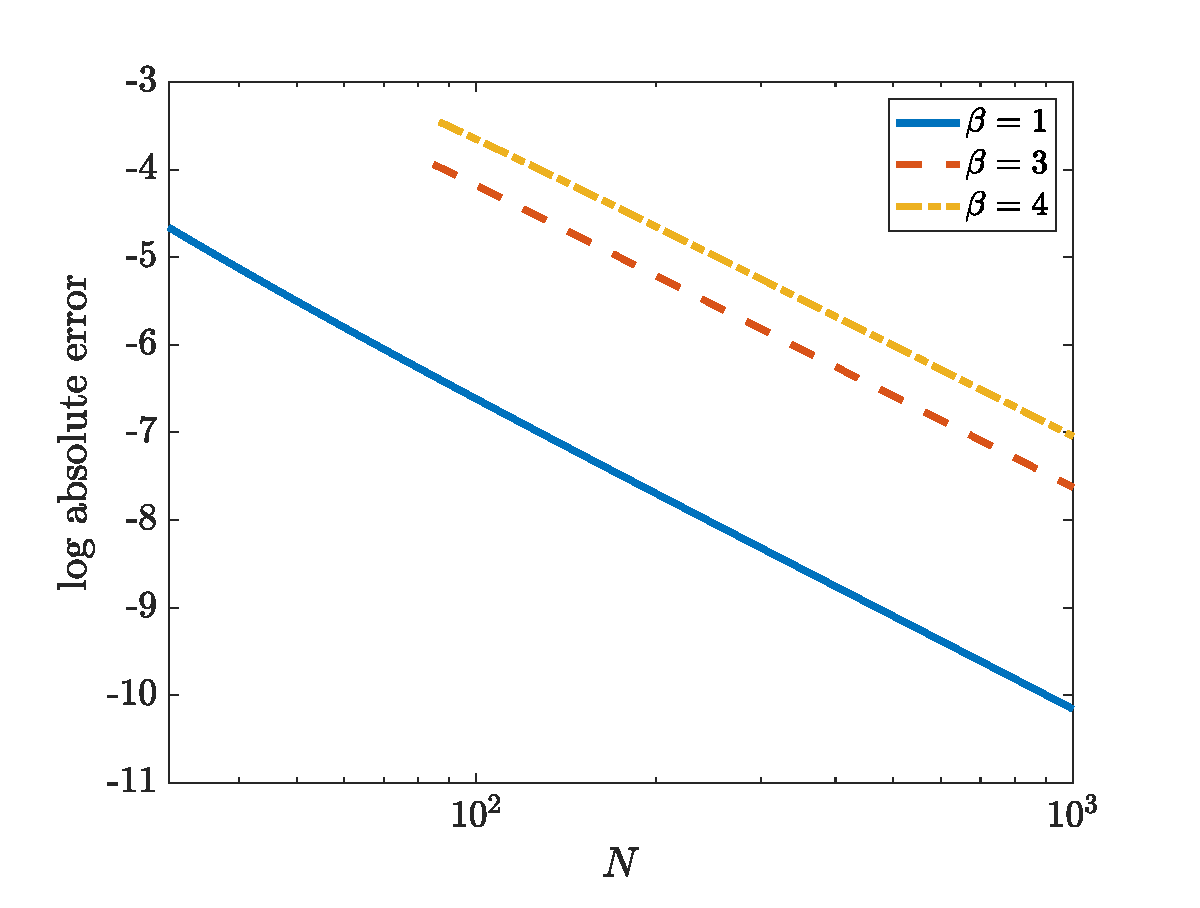
\includegraphics[width=7.8cm]{images/Hopfapproxerrorsemilog.eps} \\
    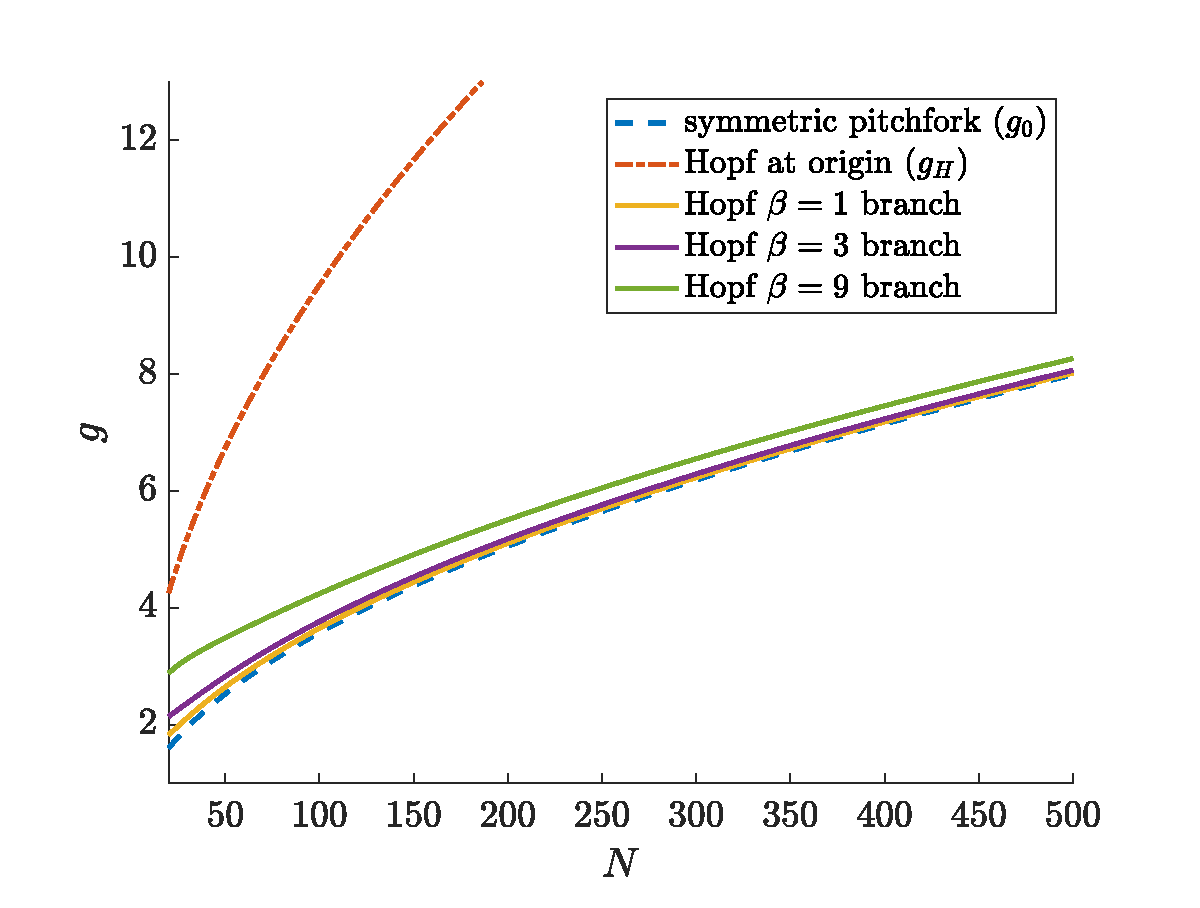
\includegraphics[width=7.8cm]{images/HopfNvsg.eps} &
    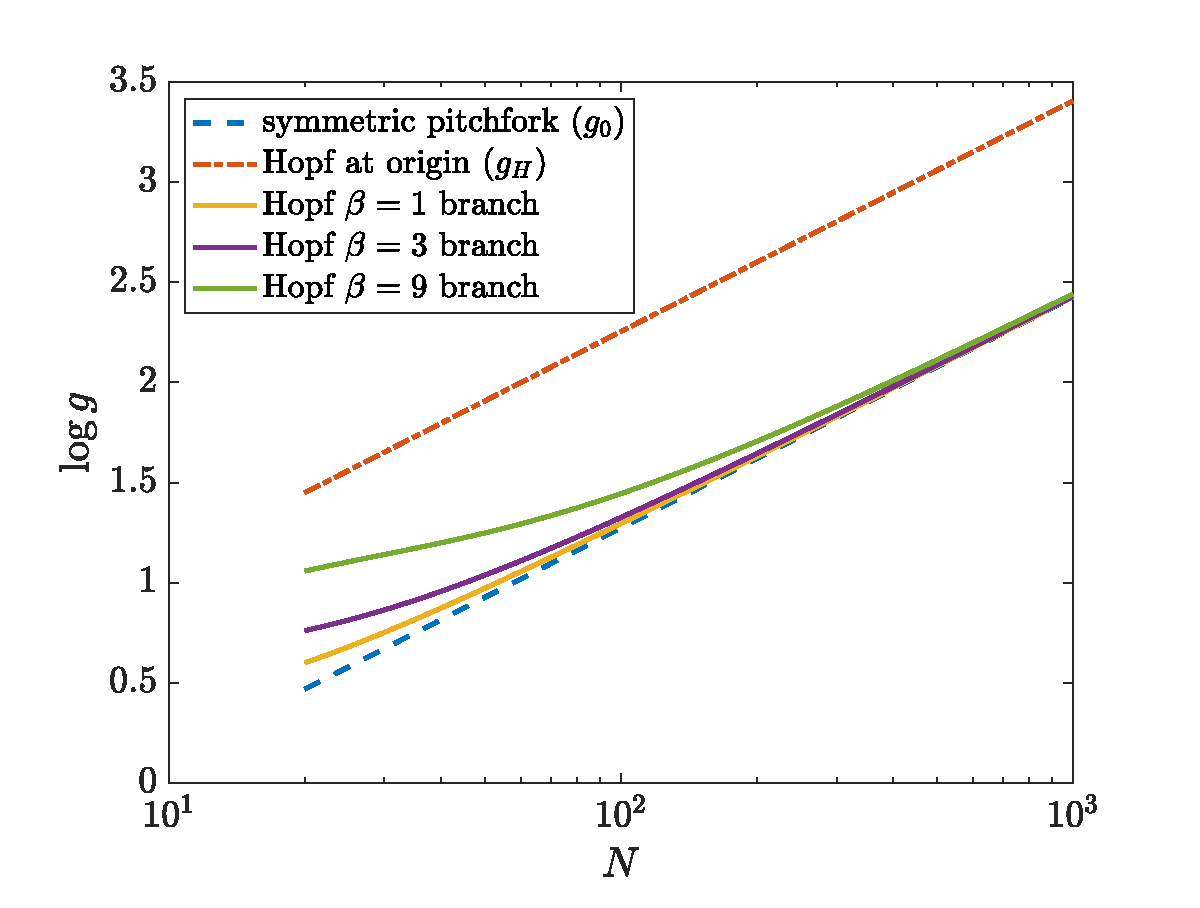
\includegraphics[width=7.8cm]{images/HopflogNvsgsemilog.eps}
    \end{tabular}
    \caption{Top left compares approximation \cref{eq:ghopfformula} to computed location of Hopf bifurcation for $I_1/I_2$ branch with $\beta = 1$. Top right plots is semi-log plot of log of absolute error of approximation \cref{eq:ghopfformula} vs $N$ for $\beta = 1$, 3, and 4. Slope of line is approximately -1.5 for all three $\beta$. Bottom left shows location in $(N, g)$ space of symmetric pitchfork bifurcation at $g_0$ (dashed line), Hopf bifurcation at origin at $g_H$ (dash-dotted line), and Hopf bifurcations on $I_1/I_2$ branches for select $\beta$ (solid lines, arranged from bottom to top in increasing $\beta$). Right panel is same data on a semi-log plot. $\alpha = 4$, $\mu_{EE}= 0.7$. }
    \label{fig:Hopfplots}
\end{figure}

% At the Hopf bifurcation, the imaginary part of eigenvalue scales as $\sqrt{N}$, which is the frequency of oscillation of the limit cycle.

\subsection{Periodic solutions}\label{sec:periodic}

Limit cycles arise as the bifurcation parameter $g$ passes through each Hopf bifurcation point. First, we discuss the limit cycle which bifurcates from the origin at $g = g_H$. Numerical computation with AUTO suggests that this limit cycle exists for all $g > g_H$, and that all excitatory cells are synchronized and all inhibitory cells are synchronized within this limit cycle. Since $n_{I_1} = n_I$ and $n_{I_2} = 0$, we will call this the $\beta=\infty$ limit cycle. 
\begin{figure}
    \centering
    \begin{tabular}{cc}
    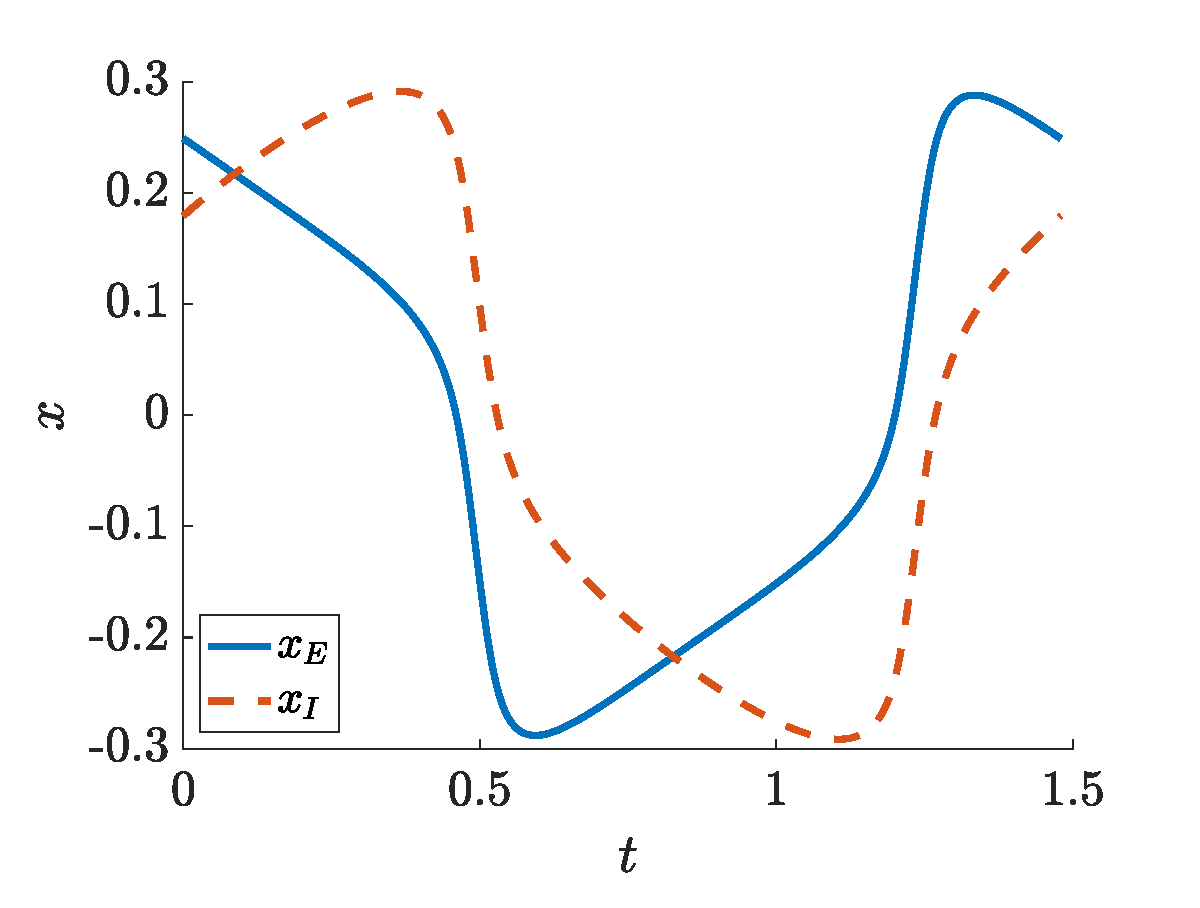
\includegraphics[width=7.85cm]{images/limitcycle1.eps}
    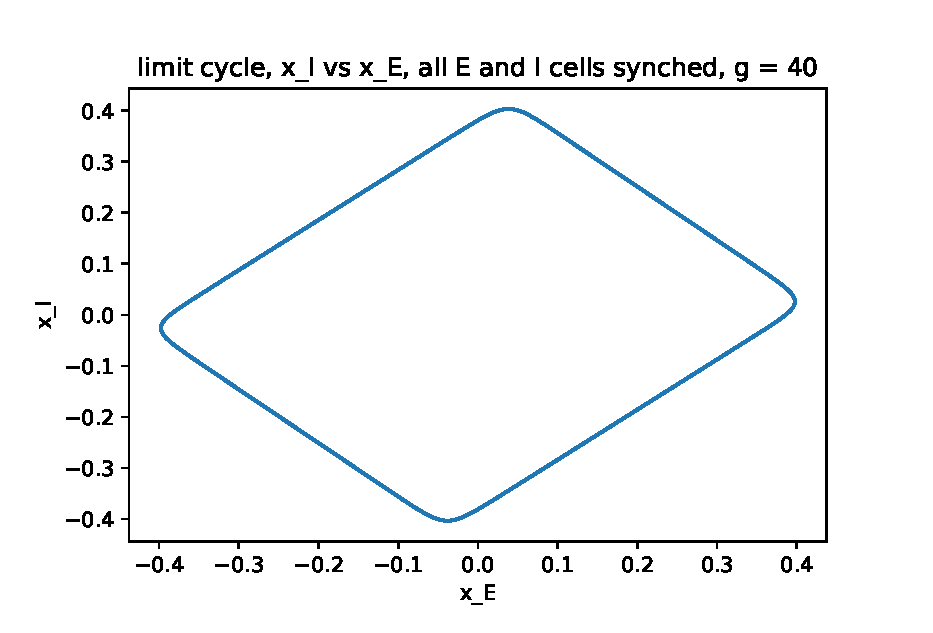
\includegraphics[width=7.85cm]{images/limitcycle2.eps}
    \end{tabular}
    \caption{$\beta = \infty$ limit cycle arising from Hopf bifurcation at $g = g_H$. Single excitatory cluster with activity $x_E(t)$, single inhibitory cluster with activity $x_I(t)$. $g = 15$, $\alpha = 4$, $\mu_{EE}= 0.7$. Period of limit cycle is 1.62.} 
    \label{fig:limitcycleorigin}
\end{figure}

In the following proposition, we prove that the $\beta=\infty$ limit cycle exists for $g > g_H$. The proof uses the Poincar\'e-Bendixson theorem, and is deferred to \cref{sec:limitcycleproof}. We note that the proposition does not address stability of the limit cycle.

\begin{proposition}\label{prop:limitcycle}
For $g > g_H$, the system \cref{eqn:sys_Basic} has a limit cycle in which all excitatory cells are synchronized, and inhibitory cells are synchronized.
\end{proposition}

In addition to the $\beta = \infty$ limit cycle, periodic orbits arise at the Hopf bifurcation on each $I_1/I_2$ branch as $g$ increases through the bifurcation point. For a given $I_1/I_2$ branch, the associated periodic orbit has the same symmetry as that branch, i.e. all excitatory cells are synchronized, and the inhibitory cells are divided into two clusters of size $n_{I_1}$ and $n_{I_2}$. For that reason, we can classify these periodic orbits in terms of the ratio $\beta = n_{I_1}/n_{I_2}$. A plot of the period of these limit cycles with increasing $g$ is shown in \cref{fig:periodvsg} for $N=20$ (see also \cite[Fig. 2]{Barreiro2017}) and \cref{fig:periodvsg50} for $N=50$. There is a critical value $g = g^*$ where all of the limit cycle branches meet. For $g > g^*$, the only remaining limit cycle is the $\beta = \infty$ limit cycle, which has become stable. The point $g = g^*$ is a symmetric pitchfork bifurcation of limit cycles, which we can see by examining the Floquet multipliers of the linearization about the $\beta = \infty$ limit cycle branch (see right panel of \cref{fig:periodvsg}). These Floquet multipliers are computed using AUTO and are all real. In addition to a single Floquet multiplier at 1 which is always present, there is a Floquet multiplier $\rho_E$ with multiplicity $n_E - 1$, a Floquet multiplier $\rho_I$ with multiplicity $n_I - 1$, and Floquet multiplier $\rho_1$ with multiplicity 1. At $g = g^*$, the $n_I - 1$ Floquet multipliers $\rho_I$ pass through 1. When this happens, as $g$ decreases though $g^*$, the $\beta = \infty$ limit cycle loses stability and gives rise to limit cycles with symmetry corresponding to each $I_1/I_2$ branch. This is analogous to the pitchfork bifurcation of the fixed point $\xvec = 0$ at $g = g_0$, which loses stability when the eigenvalue $\lambda_I$ with multiplicity $n_I - 1$ passes through the origin.

\begin{figure}
    \centering
    % \begin{tabular}{cc}
    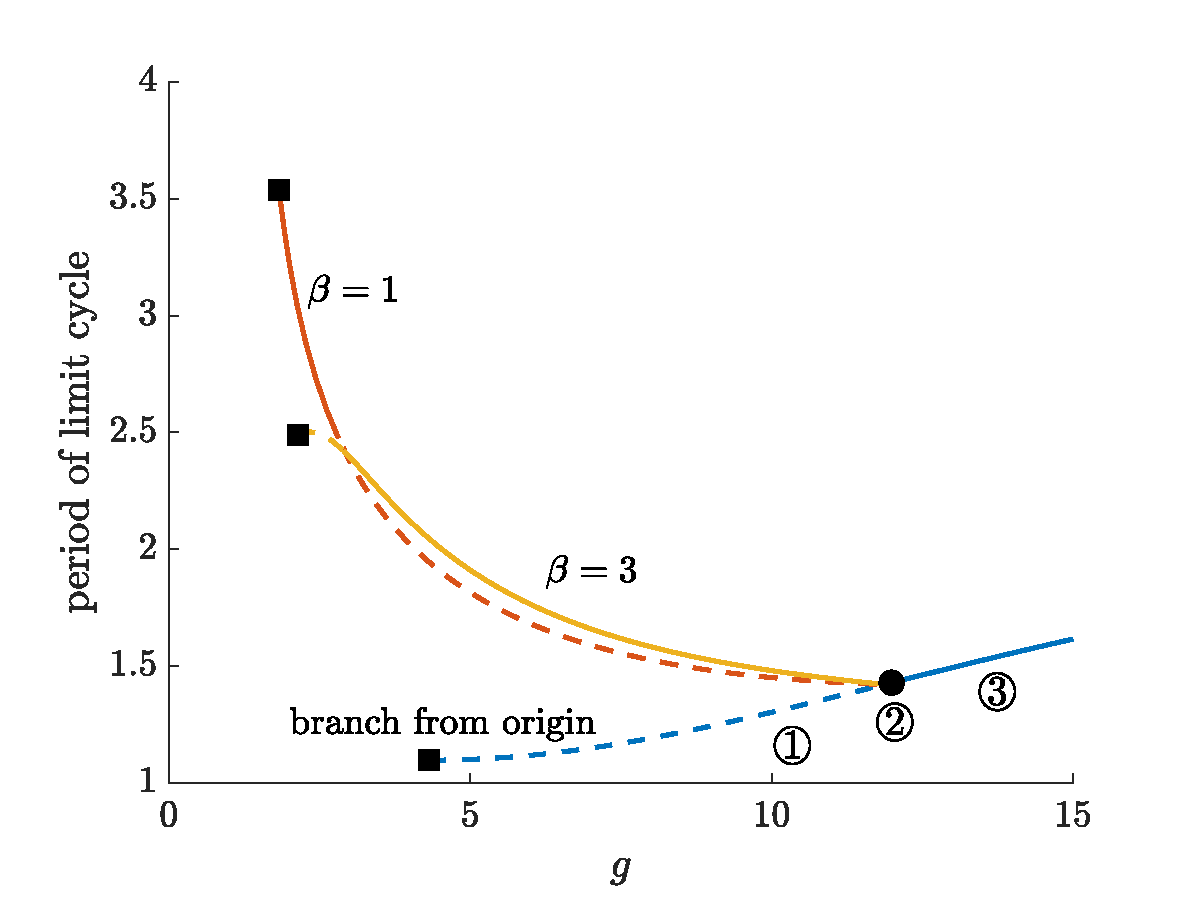
\includegraphics[width=7.8cm]{images/periodvsg}
    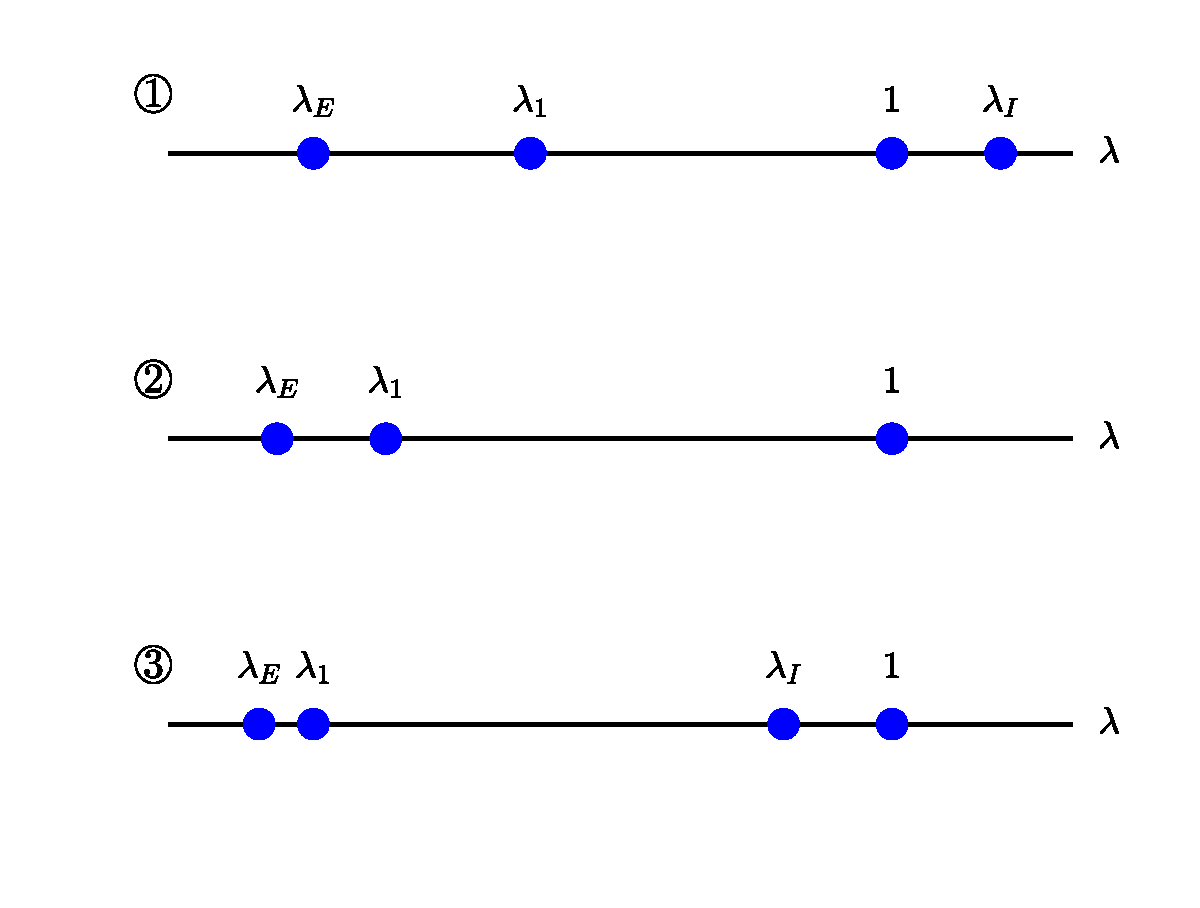
\includegraphics[width=7.8cm]{images/floquet1.eps}
    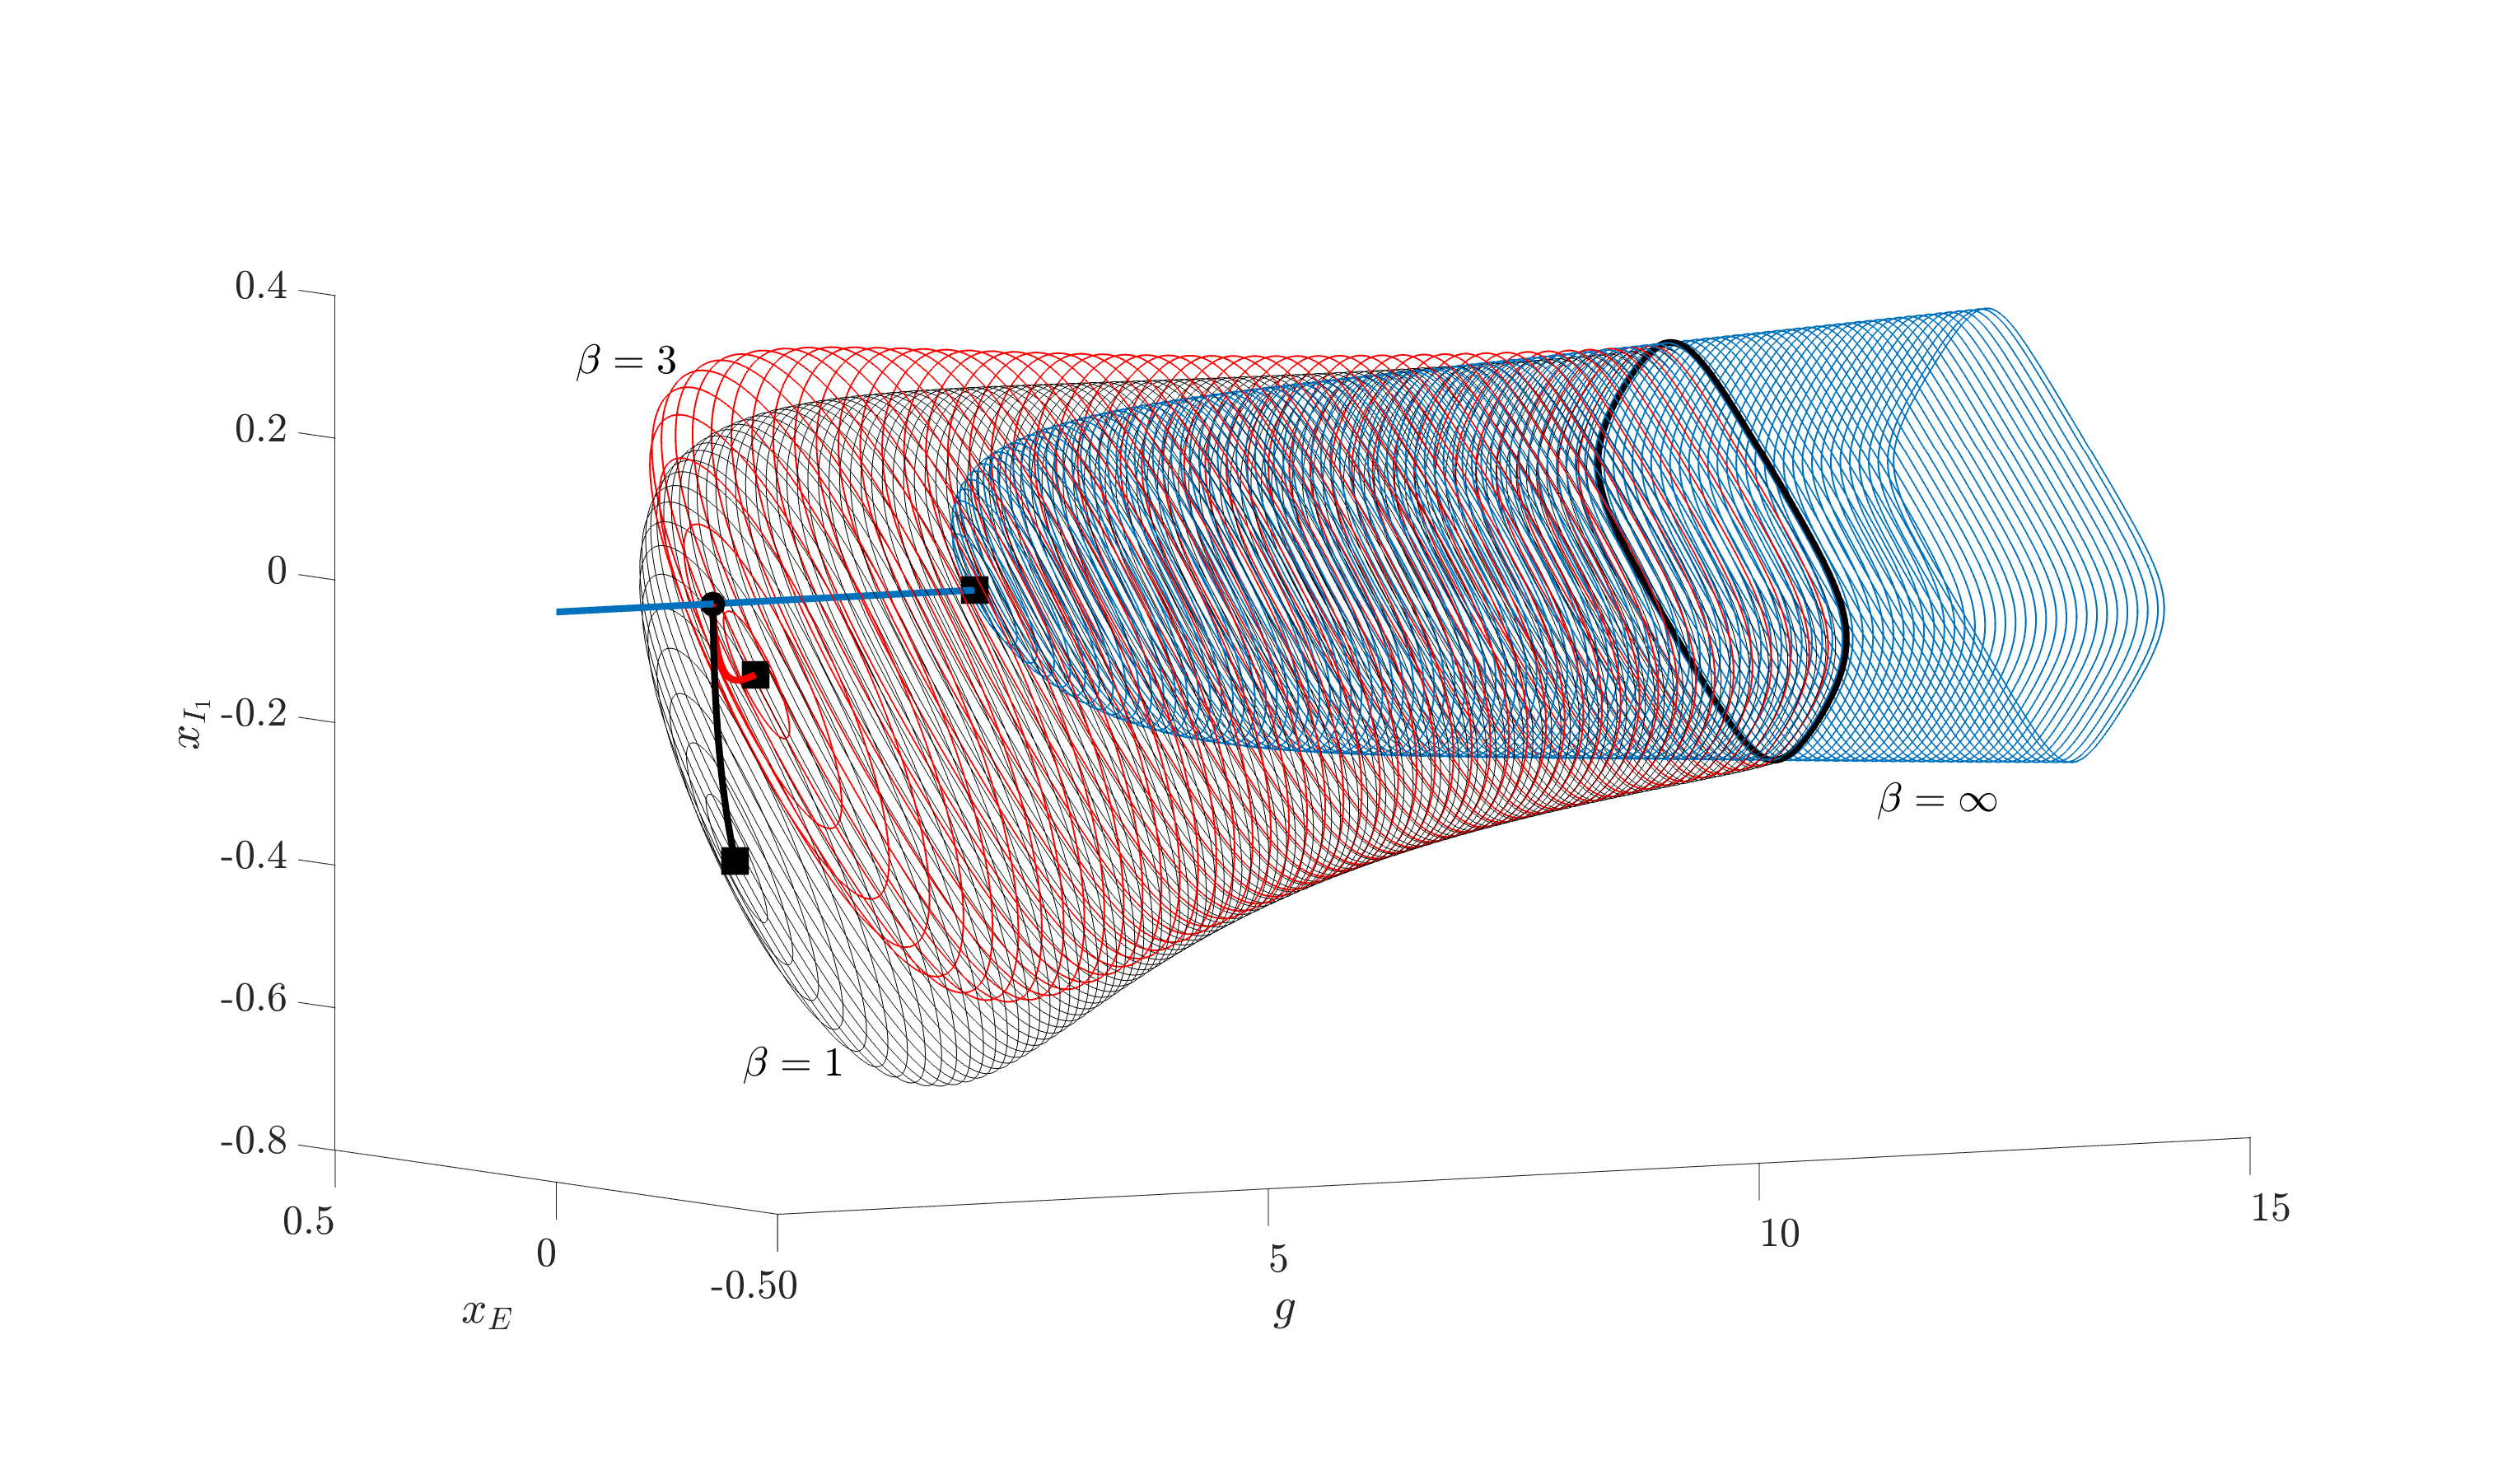
\includegraphics[width=16cm]{images/pitchbif.eps}
    % \end{tabular}
    \caption{Top left plots period of limit cycle versus $g$ for periodic solutions arising from Hopf bifurcations. Stable limit cycles indicated with solid lines. Symmetric pitchfork of limit cycles is indicated with filled circle. Hopf bifurcations indicated with filled squares, which correspond to Hopf bifurcation points in \cref{fig:noclusterBD1}. Corresponding Floquet eigenvalue pattern along $\beta = \infty$ branch is shown in top right. Bottom panel plots $x_{I_1}$ and $x_E$ vs. $g$ and shows pitchfork bifurcation at $g_0$ (filled circle), Hopf bifurcations for $\beta = 1$, $\beta = 3$, and $\beta = \infty$ (filled squares), and pitchfork bifurcation of limit cycles (dark band) at $g = g^*$. $N = 20$,  $\alpha = 4$, $\mu_{EE} = 0.7$.}
    \label{fig:periodvsg}
\end{figure}

\begin{figure}
    \centering
    % \begin{tabular}{cc}
    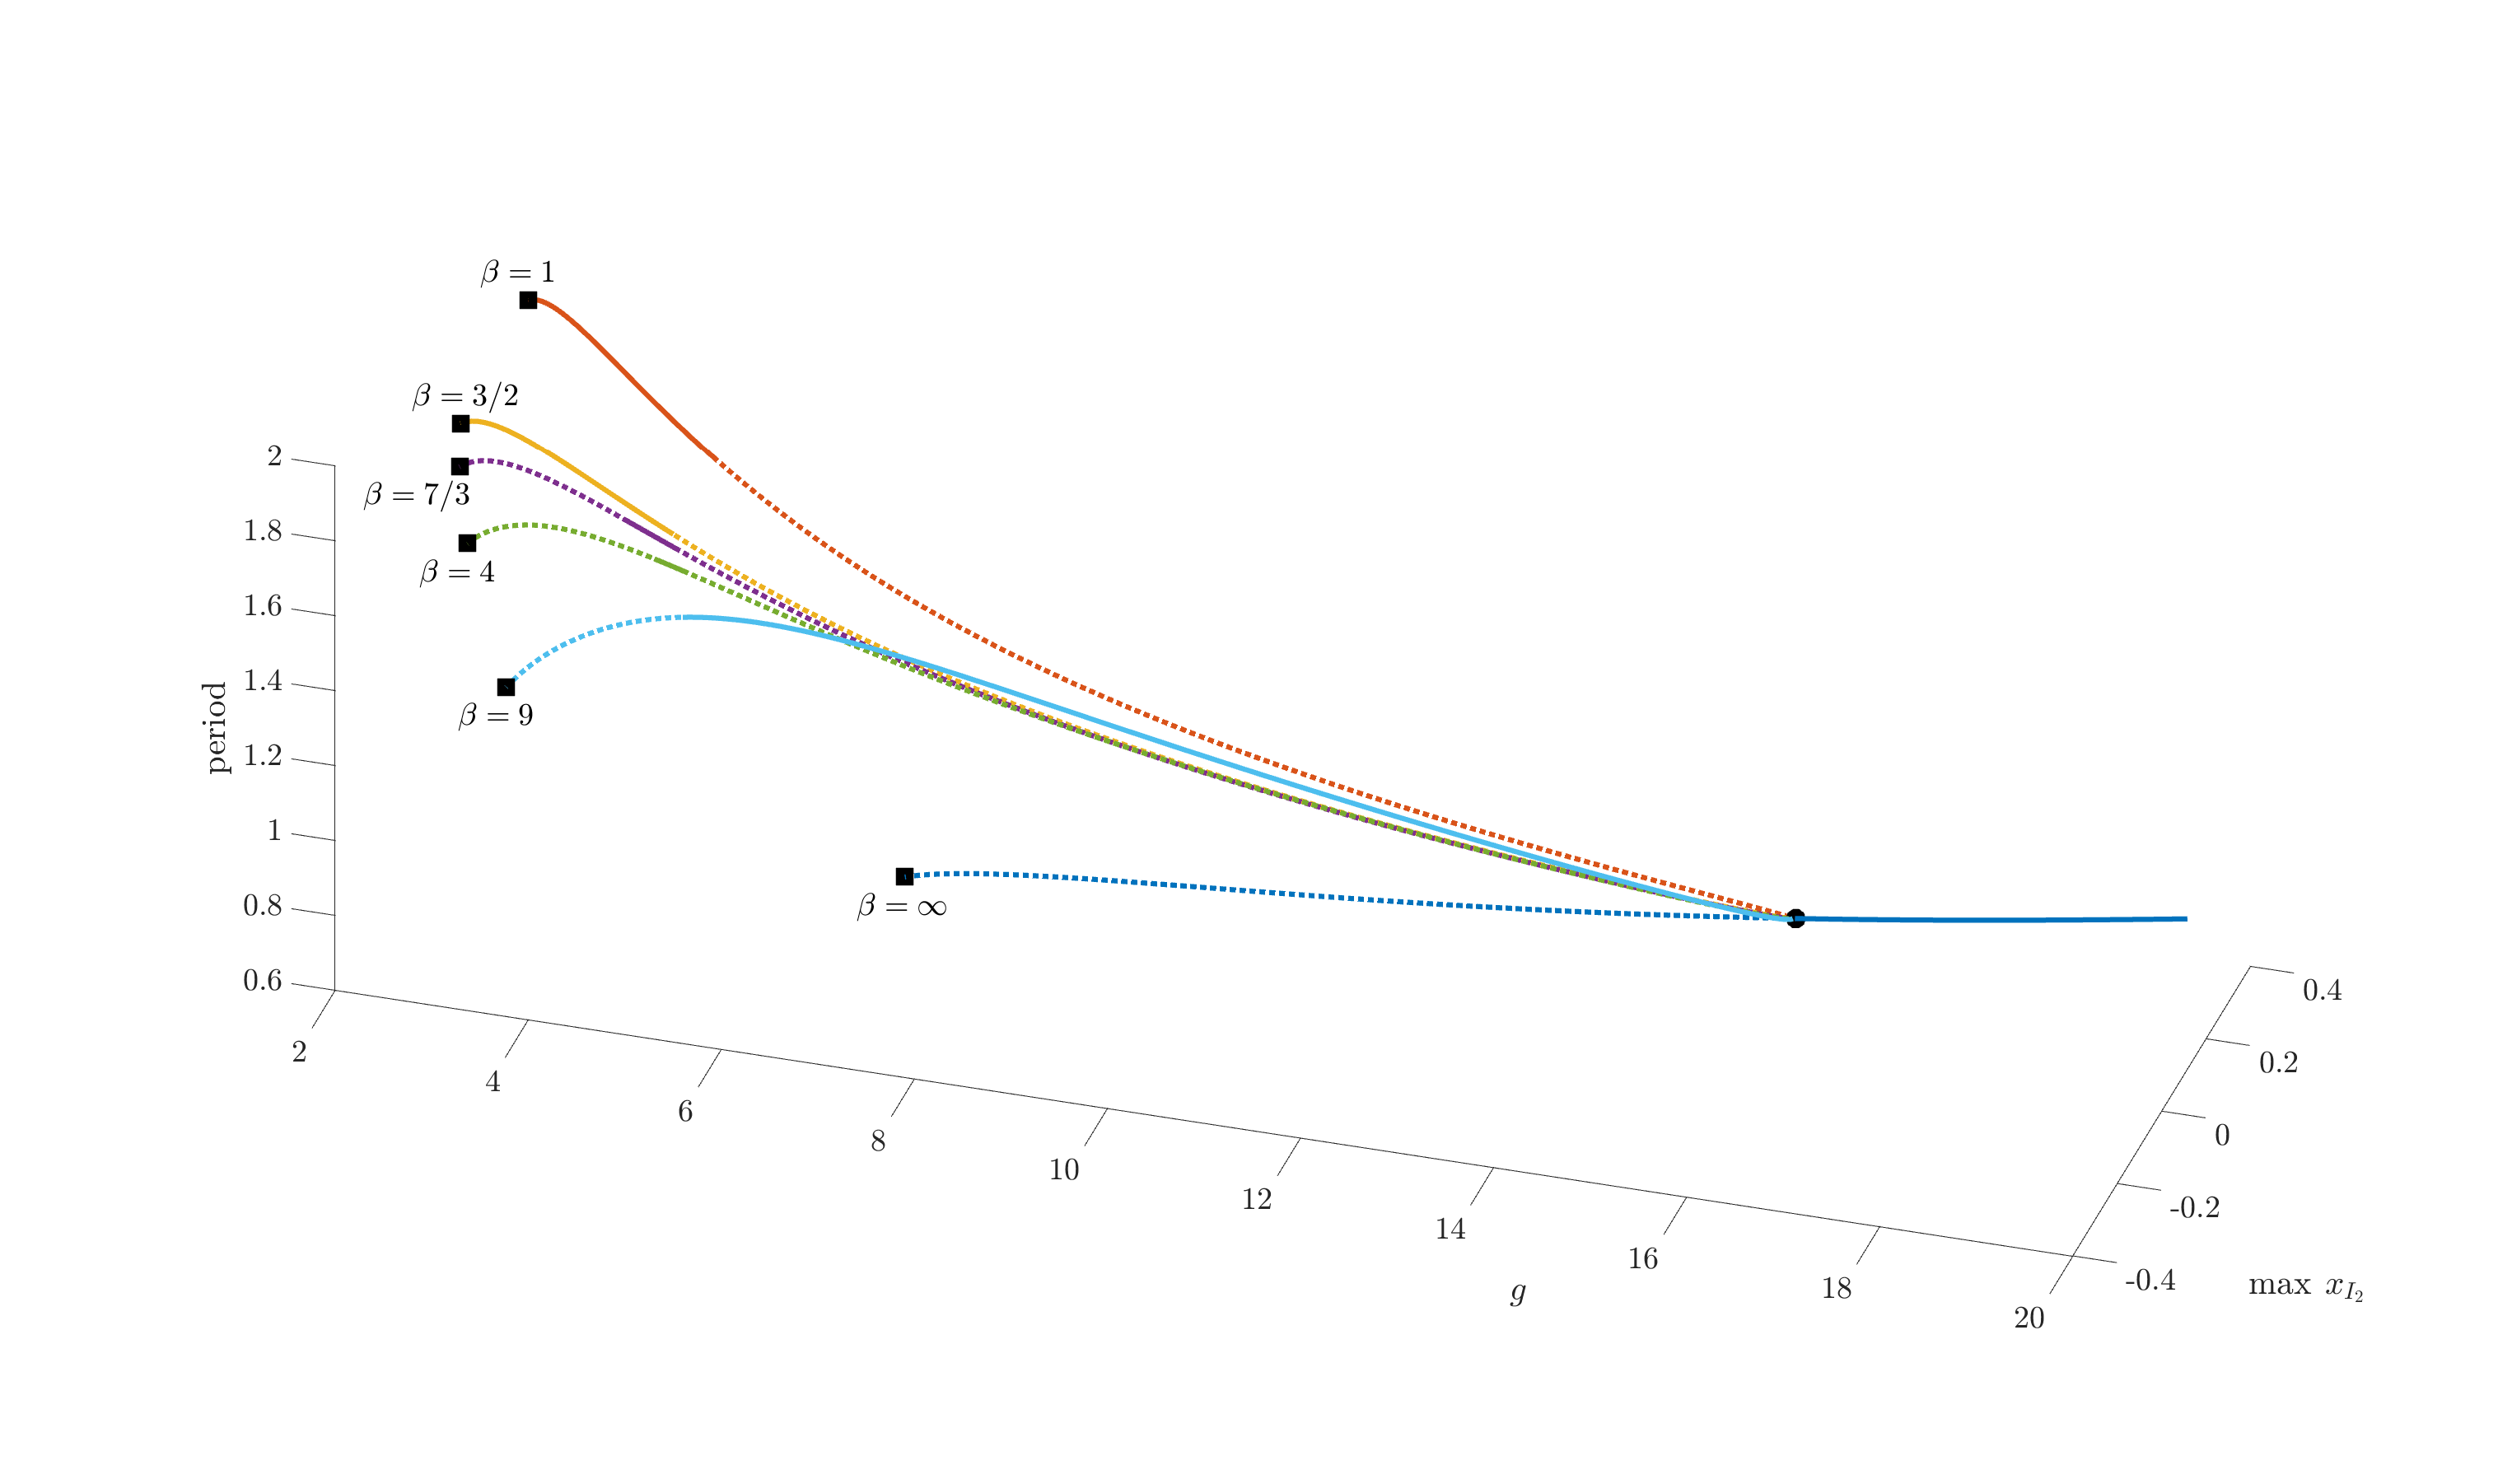
\includegraphics[width=16cm]{images/periodvsgN50.eps}
    % \end{tabular}
    \caption{Period of limit cycle versus $g$ and $\max \: x_{I_2}$ for periodic solutions arising from Hopf bifurcations. Stable limit cycles indicated with solid lines. Symmetric pitchfork of limit cycles is indicated with filled circle. Hopf bifurcations indicated with filled squares. $N = 50$,  $\alpha = 4$, $\mu_{EE} = 0.7$.}
    \label{fig:periodvsg50}
\end{figure}

\subsection{Behavior of the \texorpdfstring{$I_1/I_2$}{I1/I2} branch for large \texorpdfstring{$g$}{g}}\label{sec:stab_largeg}

We have characterized the three-cluster fixed point solutions on the $I_1/I_2$ branches near the symmetric pitchfork bifurcation point at $g = g_0$. Next, we will show that these branches are unstable for sufficiently large $g$. Fix $\beta = n_{I_1}/n_{I_2}$, and let $\xvec = (x_E, x_{I_1}, x_{I_2})$ be a solution to \cref{eq:otherbranchmatrixeq} for $g > g_0$. Let $\xvec^*$ be the corresponding fixed point of \cref{eq:reducedmatrixform}. We will look at the eigenvalues of $D\tilde{F}(\xvec^*)$ for large $g$. The sum of these eigenvalues is 
\[
\text{Trace }D\tilde{F}(\xvec^*) = \frac{g (n_E-1) \mu_{EE}}{\sqrt{N}} \sech^2( g x_E ) - (n_I+1).
\]
There are two possibilities for $x_E$ as $g \rightarrow 0$. If $x_E \rightarrow 0$, then $\sech^2( g x_E ) \rightarrow s$, with $0 < s < 1$. Thus for sufficiently large $g$, $\text{Trace }D\tilde{F}(\xvec^*) > 0$, which implies that $D\tilde{F}(\xvec^*)$ has an eigenvalue with positive real part. The remaining possibility is that $x_E \rightarrow \hat{x}_E \neq 0$. We will show that this cannot occur.

Suppose $x_E \rightarrow \hat{x}_E \neq 0$ as $g \rightarrow \infty$. Without loss of generality, we can take $\hat{x}_E > 0$, since by odd symmetry of \cref{eqn:sys_Basic}, there will be a corresponding solution with $\hat{x}_E < 0$. This implies that $\tanh x_{E} \rightarrow 1$. There are four cases to consider:\\
\begin{itemize}
    \item Case 1: $x_{I_1} \rightarrow \hat{x}_{I_1} \neq 0$ and $x_{I_2} \rightarrow \hat{x}_{I_2} \neq 0$.
    \item Case 2: $x_{I_1} \rightarrow \hat{x}_{I_1} \neq 0$ and $x_{I_2} \rightarrow 0$.
    \item Case 3: $x_{I_1} \rightarrow 0$ and $x_{I_2} \rightarrow \hat{x}_{I_2} \neq 0$.
    \item Case 4: $x_{I_1} \rightarrow 0$ and $x_{I_2} \rightarrow 0$.\\
\end{itemize}

The computations to follow were done with the assistance of Wolfram Mathematica. For Case 1, $\tanh(g x_{I_1}) \rightarrow \pm 1$ and $\tanh(g x_{I_2}) \rightarrow \pm 1$. We can then use \cref{eq:otherbranchmatrixeq} to solve for $(\hat{x}_E, \hat{x}_{I_1}, \hat{x}_{I_2})$. The signs of these solutions are all inconsistent, as we can see in \cref{table:signtable}. 

\begin{table}
\centering
    \begin{tabular}{llll}
        \toprule
        sgn $(\hat{x}_E, \hat{x}_{I_1}, \hat{x}_{I_2})$ & $\frac{\sqrt{N}}{\mu_{EE}}\hat{x}_E$ & $\frac{\sqrt{N}}{\mu_{EE}}\hat{x}_{I_1}$ & $\frac{\sqrt{N}}{\mu_{EE}}\hat{x}_{I_2}$ \\
        \midrule
        $(1,1,1)$   & $-1 < 0$ & $\alpha$ & $\alpha$ \\
        $(1,-1,-1)$ & $2 \alpha n_I - 1$ & $\alpha(2 n_I - 1) > 0 $ & $\alpha(2 n_I - 1) > 0$ \\
        $(1,1,-1)$  & $2 \alpha n_{I_2} - 1$ & $\alpha(2 n_{I_2} + 1)$ & $\alpha(2 n_{I_2} - 1) > 0$  \\
        $(1,-1,1)$  & $2 \alpha n_{I_1} - 1$ & $\alpha(2 n_{I_1} - 1) > 0$ & $\alpha(2 n_{I_1} + 1)0$  \\
        \bottomrule
    \end{tabular}
    \label{table:signtable}
    \vspace{0.25cm}
    \caption{Sign table showing that all solutions for nonzero $(\hat{x}_E, \hat{x}_{I_1}, \hat{x}_{I_2})$ are inconsistent.}
\end{table}

For Case 2, if $\tanh( g \hat{x}_{I_2} ) \rightarrow 0$, the solution $(\hat{x}_E, \hat{x}_{I_1}, \hat{x}_{I_2})$ from \cref{eq:otherbranchmatrixeq} is inconsistent using the same argument as in Case 1. The only remaining possibility is $\tanh( g \hat{x}_{I_2} ) \rightarrow \hat{y}_{I_2}$, where $0 < |\hat{y}_{I_2}| < 1$. In the limit $g \rightarrow \infty$, \cref{eq:otherbranchmatrixeq} becomes
\begin{equation*}
 \begin{aligned}
 \begin{bmatrix} \hat{x}_E \\ \hat{x}_{I_1} \\ 0 \end{bmatrix} 
 &= \frac{\mu_{EE}}{\sqrt{N}} 
 \begin{bmatrix} (\alpha n_I - 1) & -\alpha \frac{\beta}{\beta+1} n_I & - \alpha \frac{1}{\beta+1} n_I  \\
    \alpha n_I  & -\alpha \left(\frac{\beta}{\beta+1} n_I-1\right) & - \alpha \frac{1}{\beta+1} n_I  \\
    \alpha n_I & -\alpha \frac{\beta}{\beta+1} n_I & -\alpha \left(\frac{1}{\beta+1} n_I-1\right)
 \end{bmatrix}
 \begin{bmatrix} 1 \\ \pm 1 \\ \hat{y}_{I_2} \end{bmatrix}.
 \end{aligned}
 \end{equation*}
The consistency condition (from the third row) can only be satisfied if $\hat{y}_{I_2} = \frac{n_I}{n_I - (\beta + 1)} > 1$ (for $\hat{x}_{I_1} > 0$) or $\hat{y}_{I_2} = \frac{n_I(1 + 2 \beta)}{n_I - (\beta + 1)} > 1$ (for $\hat{x}_{I_1} < 0$), both of which are impossible. Case 3 is similar.

For Case 4, if $\tanh( g \hat{x}_{I_1} ) \rightarrow 0$ or $\tanh( g \hat{x}_{I_2} ) \rightarrow 0$, the solution $(\hat{x}_E, \hat{x}_{I_1}, \hat{x}_{I_2})$ from \cref{eq:otherbranchmatrixeq} is inconsistent using the same argument as in Case 1. The remaining possibility is $\tanh( g \hat{x}_{I_1} ) \rightarrow \hat{y}_{I_1}$  and $\tanh( g \hat{x}_{I_2} ) \rightarrow \hat{y}_{I_2}$, where $0 < |\hat{y}_{I_1}| , |\hat{y}_{I_2}| < 1$. In the limit $g \rightarrow \infty$, \cref{eq:otherbranchmatrixeq} becomes
\begin{equation*}
 \begin{aligned}
 \begin{bmatrix} \hat{x}_E \\ 0 \\ 0 \end{bmatrix} 
 &= \frac{\mu_{EE}}{\sqrt{N}} 
 \begin{bmatrix} (\alpha n_I - 1) & -\alpha \frac{\beta}{\beta+1} n_I & - \alpha \frac{1}{\beta+1} n_I  \\
    \alpha n_I  & -\alpha \left(\frac{\beta}{\beta+1} n_I-1\right) & - \alpha \frac{1}{\beta+1} n_I  \\
    \alpha n_I & -\alpha \frac{\beta}{\beta+1} n_I & -\alpha \left(\frac{1}{\beta+1} n_I-1\right)
 \end{bmatrix}
 \begin{bmatrix} 1 \\ \hat{y}_{I_1} \\ \hat{y}_{I_2} \end{bmatrix}.
 \end{aligned}
 \end{equation*}
 The consistency conditions (from the second and third rows) can only be satisfied if $\hat{y}_{I_1} = \hat{y}_{I_2} = \frac{n_I}{n_I - 1} > 1$, which is impossible.

\section{Excitatory clusters, weight parameters balanced}

We now allow the excitatory cells to be grouped into $n_C$ clusters of size $p$, where $p = \lfloor N f/n_C \rfloor$. We will take $p > 1$ to ensure that each excitatory cluster contains more than one cell, and we will also assume $n_C \geq \alpha$ (e.g. $n_C > 4$ for the standard value of $\alpha = 4$). Since we are interested in the behavior of the system for large $N$ and for a large number of clusters (e.g. $N_c$ scales with $\sqrt{N}$), this is not a significant restriction. Cells will be connected within, but not between, clusters. The matrix $H$ is now
\begin{equation}\label{eq:Hcluster}
H = \frac{1}{\sqrt{N}}
\left[ 
\begin{blockarray}{ccccc}
\begin{block}{cccc|c}
\mu_{EE}\Kvec_{p} & 0 & \hdots & 0 & \BAmulticolumn{4}{c}{\multirow{4}{*}{$\mu_{EI}\Onevec_{n_E \times n_I}$}}\\
0 & \mu_{EE} \Kvec_{p} & \hdots & 0 &&&&\\
\vdots & \vdots & \ddots & 0 &&&&\\
0 & 0 & \hdots & \mu_{EE} \Kvec_{p} &&&&\\
\end{block} 
\cline{1-8}
\begin{block}{cccc|c}
&&&&\\
\BAmulticolumn{4}{c|}{\mu_{IE}\Onevec_{n_I \times n_E}} & \mu_{II} \Kvec_{n_I}\\
\end{blockarray}
\right]
\end{equation}
which is associated with the symmetry group
\begin{align*}
\Gamma &= \underbrace{S_{p} \oplus \cdots  \oplus S_{p}}_{n_C} \oplus \, S_{n_I} && p = fN/n_C.
\end{align*}
As in the previous section, we choose the weights so that the network is balanced. 
\begin{align*}
\mu_{EE} &= n_C \mu && \mu_{IE} = \mu \\
\mu_{EI} &= -\alpha \mu && \mu_{II} = -\alpha.
\end{align*}
The expression for $\mu_{EE}$ compensates for the fact that each excitatory cell has fewer excitatory connections. The eigenvalues of $H$ (middle panel of \cref{fig:Heigpattern}) are:
\begin{itemize}
\item $\lambda_I := \alpha \mu > 0$ with multiplicity $n_I - 1$
\item $\lambda_E := -n_C \mu < 0$ with multiplicity $(p-1) \times n_C = n_E - n_C$.
\item $\lambda_C := (p-1) n_C \mu > 0$, with multiplicity $n_C - 1$.
\item A complex conjugate pair of eigenvalues $\lambda_0 \pm i \omega_0$, with 
\begin{equation*}
    \lambda_0 := \frac{1}{2}\mu(\alpha - n_C), \quad 
    \omega_0 := \frac{1}{2}\mu \sqrt{ \alpha + n_C} \sqrt{ n_C(4 p - 1) - \alpha },
\end{equation*}
where we used the fact that $\alpha n_I = n_E = p n_C$.
\end{itemize}
Since $\lambda_E < 0$ and $\lambda_0 \leq 0$ (as a consequence of taking $n_C \geq \alpha$), the corresponding eigenvalues of $DF(0)$ will always be negative, and thus will not affect stability of the fixed point at 0. The eigenvalues which determine stability of the origin are $\lambda_I$ and $\lambda_C$. We note that since $p > 1$, $0 < \lambda_I < \lambda_C$.

As the bifurcation parameter $g$ increases from 0, the set of eigenvalues $\lambda_C^*(g)$ of $DF(0)$ corresponding to $\lambda_C$ cross the imaginary axis first at 
\begin{equation}
    g = g_C := \frac{\sqrt{N}}{(p-1) n_C \mu}.
\end{equation}
When this occurs, the origin loses stability in a symmetric pitchfork bifurcation, similar to what occurs with the inhibitory cells in the previous section. As $g$ is further increased, the eigenvalue $\lambda_I^*(g)$ crosses the imaginary axis at $g = g_0$, where $g_0$ is defined by \cref{eq:pitchlocation}. Another symmetric pitchfork bifurcation occurs at this point, this time involving the inhibitory cells. An important distinction from the previous section is that there will be no Hopf bifurcation at the origin, since the complex conjugate pair of eigenvalues cannot cross the imaginary axis.

As in the previous section, it follows from Equivariant Bifurcation Theorem that there is a branch of solutions emerging at the bifurcation point $g = g_C$ for any possible division of excitatory clusters into exactly two groups of clusters. All cells are synchronized within each excitatory cluster. Each such branch may be characterized by the number $\beta_C = n_{C_1}/n_{C_2}$, which gives the ratio of the sizes of the two groups of excitatory clusters. Without loss of generality, we may take $n_{C_1} \geq n_{C_2}$, so that $\beta_C \geq 1$. At the start of each $C_1/C_2$ branch, the inhibitory cells are synchronized, since near $g = g_C$, no other eigenvalues have crossed through the origin yet, thus no bifurcations involving the inhibitory cells have  occurred. The solution on each $C_1/C_2$ branch is then given as $(x_{E_1}, x_{E_2}, x_{I})$. Due to the odd symmetry of \cref{eqn:sys_Basic}, there is a corresponding $C_1/C_2$ branch for each $\beta_C$ with solution $(-x_{E_1}, -x_{E_2}, -x_{I})$., which we will ignore for simplicity.


\subsection{Solutions on \texorpdfstring{$C_1/C_2$}{C1/C2} branch}

First, we derive leading order expressions for the solutions along the $C_1/C_2$ branches for $g$ close to $g_C$. The simplest case occurs when $n_C$ is even and $\beta_C = 1$, in which case $n_{C_1}=n_{C_2}$. On this branch, $x_{E_2} = -x_{E_1}$, i.e. there are two equally sized groups of excitatory clusters with equal and opposite activity, and all the inhibitory cells have synchronized activity $x_I = 0$. Taking $x_{E_1} = x_E$, $x_{E_2} = -x_E$, and $x_I = 0$ in \cref{eq:reducedsystem} and simplifying, we obtain the single equation $\tanh(g x_E) = g_C x_E$. As in the previous section, $x_E$ is given, to leading order, by
\begin{align}\label{eq:xEapprox}
x_E &= \sqrt{ \frac{3(g - g_C) }{g^3}} && g \geq g_C,
\end{align}
for $g$ close to $g_C$. For $\beta_C > 1$, we find the solution along each $C_1/C_2$ branch by reducing \cref{eqn:sys_Basic} to the 3-dimensional system
\begin{equation}\label{eq:cluster3system}
 \begin{aligned}
 \begin{bmatrix} x_{E_1} \\ x_{E_2} \\ x_{I} \end{bmatrix} 
 &= \frac{\mu}{\sqrt{N}} 
 \begin{bmatrix} 
    (p-1)n_C & 0 & -p n_C  \\
    0  & (p-1)n_C & -p n_C \\
    p n_C \frac{\beta_C}{\beta_C+1} &
    p n_C \frac{1}{\beta_C+1} &
    -(p n_C - \alpha)
 \end{bmatrix}
 \begin{bmatrix} \tanh(g x_{E_1}) \\\tanh ( g x_{E_2} ) \\\tanh(g x_{I})\end{bmatrix},
 \end{aligned}
 \end{equation}
 where we used $\alpha n_I = n_E = p n_C$. The variables $x_{E_1}$ and $x_{E_2}$ are the activities of the two groups of excitatory clusters, and $x_I$ is the activity of the inhibitory cells, which are synchronized since $g$ is close to $g_C$. As $N \rightarrow \infty$, numerical continuation with AUTO suggests that \cref{eq:cluster3system} has a solution of the form
\begin{equation}\label{eq:XE1E2asymp}
    x_{E_2} = -\beta_C x_{E_1} + \mathcal{O}\left( \frac{1}{N^2} \right), \quad 
    x_{E_1} = \mathcal{O}\left( \frac{1}{N} \right), \quad
    x_I = \mathcal{O}\left( \frac{1}{N^2} \right)
\end{equation}
for $g$ close to $g_C$. Following the same procedure as in the previous section, we obtain the formula
 \begin{align}\label{eq:XE1}
 x_{E_1} &= \pm \sqrt{ \frac{ 3(g - g_C) }{ (1 - \beta_C + \beta_C^2 )g^3}} + \mathcal{O}\left( \frac{1}{N^2}\right)&& g \geq g_C,
\end{align}
for $g$ close to $g_C$, which reduces to \cref{eq:xEapprox} when $\beta = 1$.

\begin{figure}
    \centering
    % \begin{tabular}{cc}
    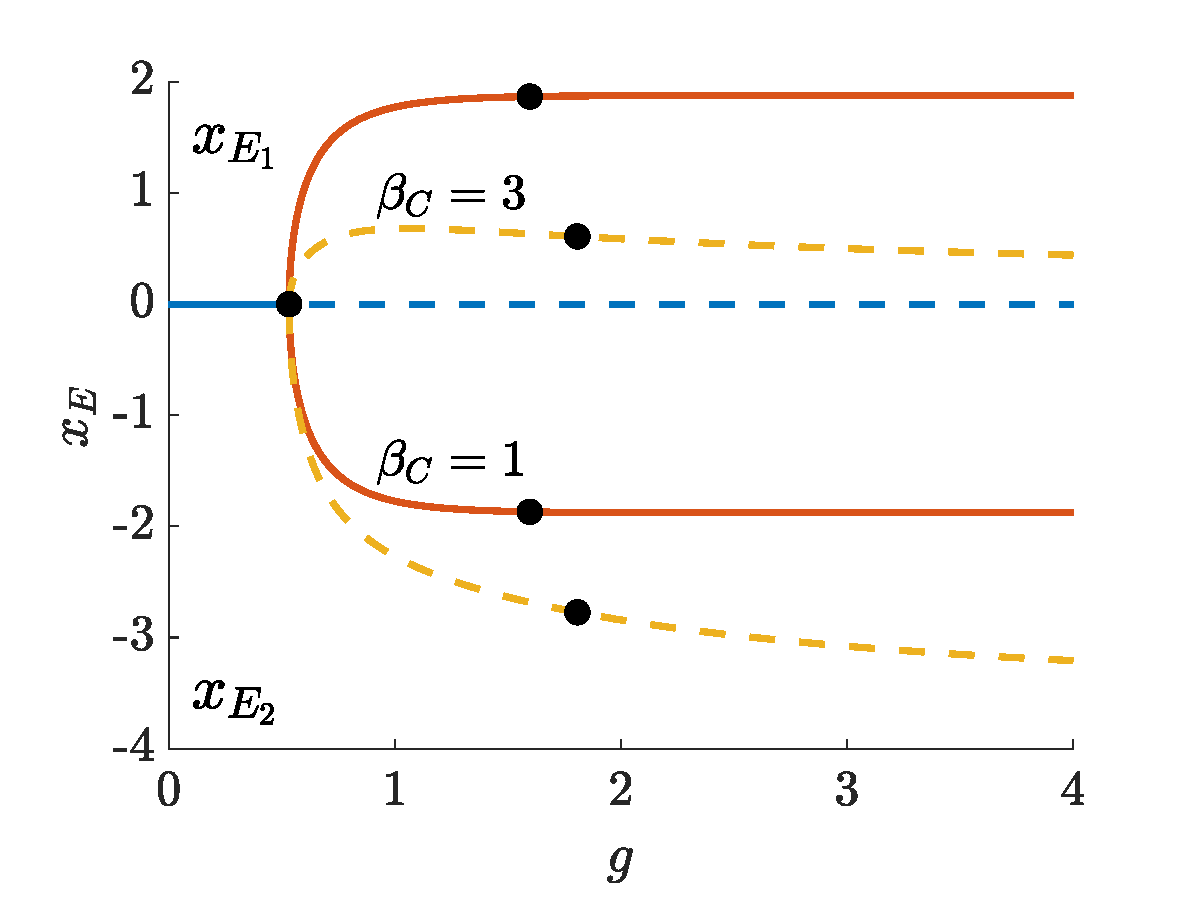
\includegraphics[width=8cm]{images/bdclusters20c4E.eps} 
    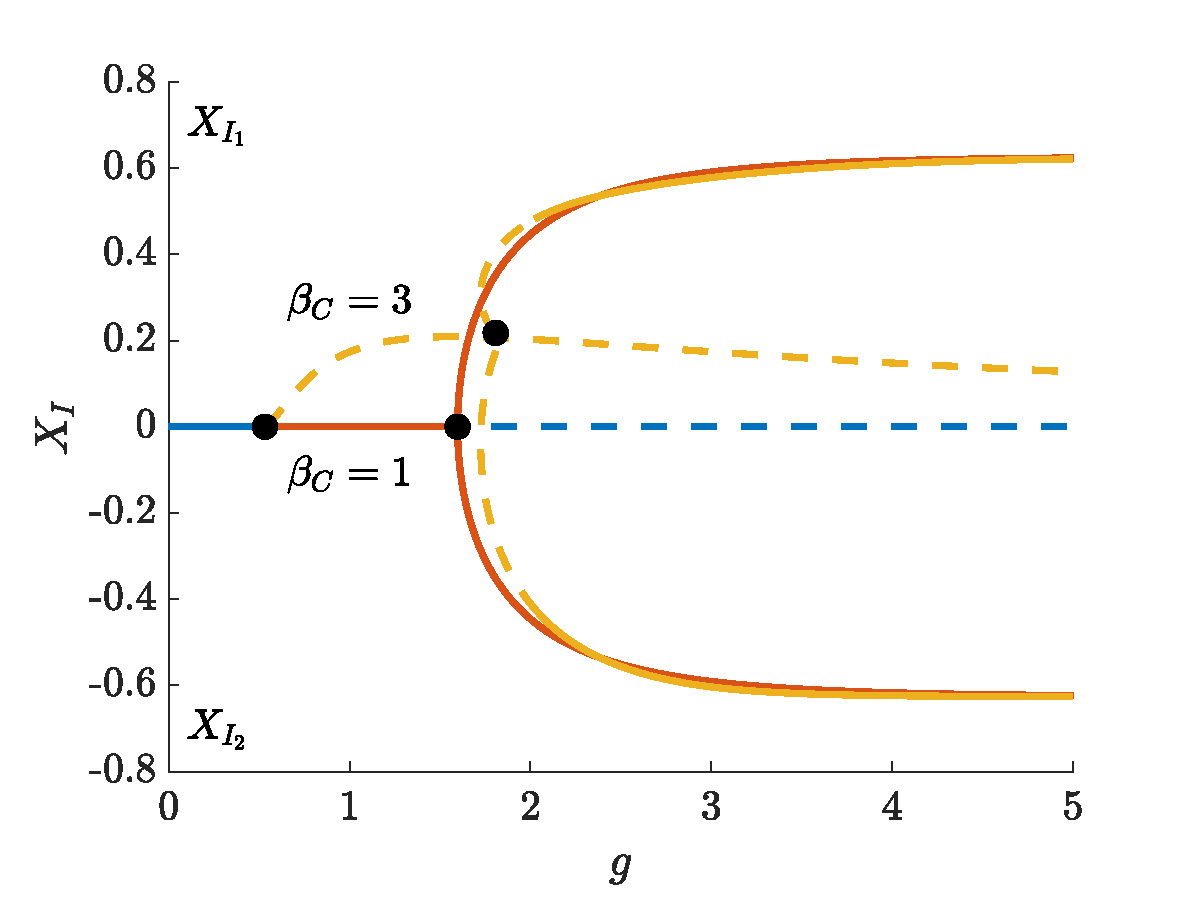
\includegraphics[width=8cm]{images/bdclusters20c4I.eps} 
    \vspace{-0.5cm}
    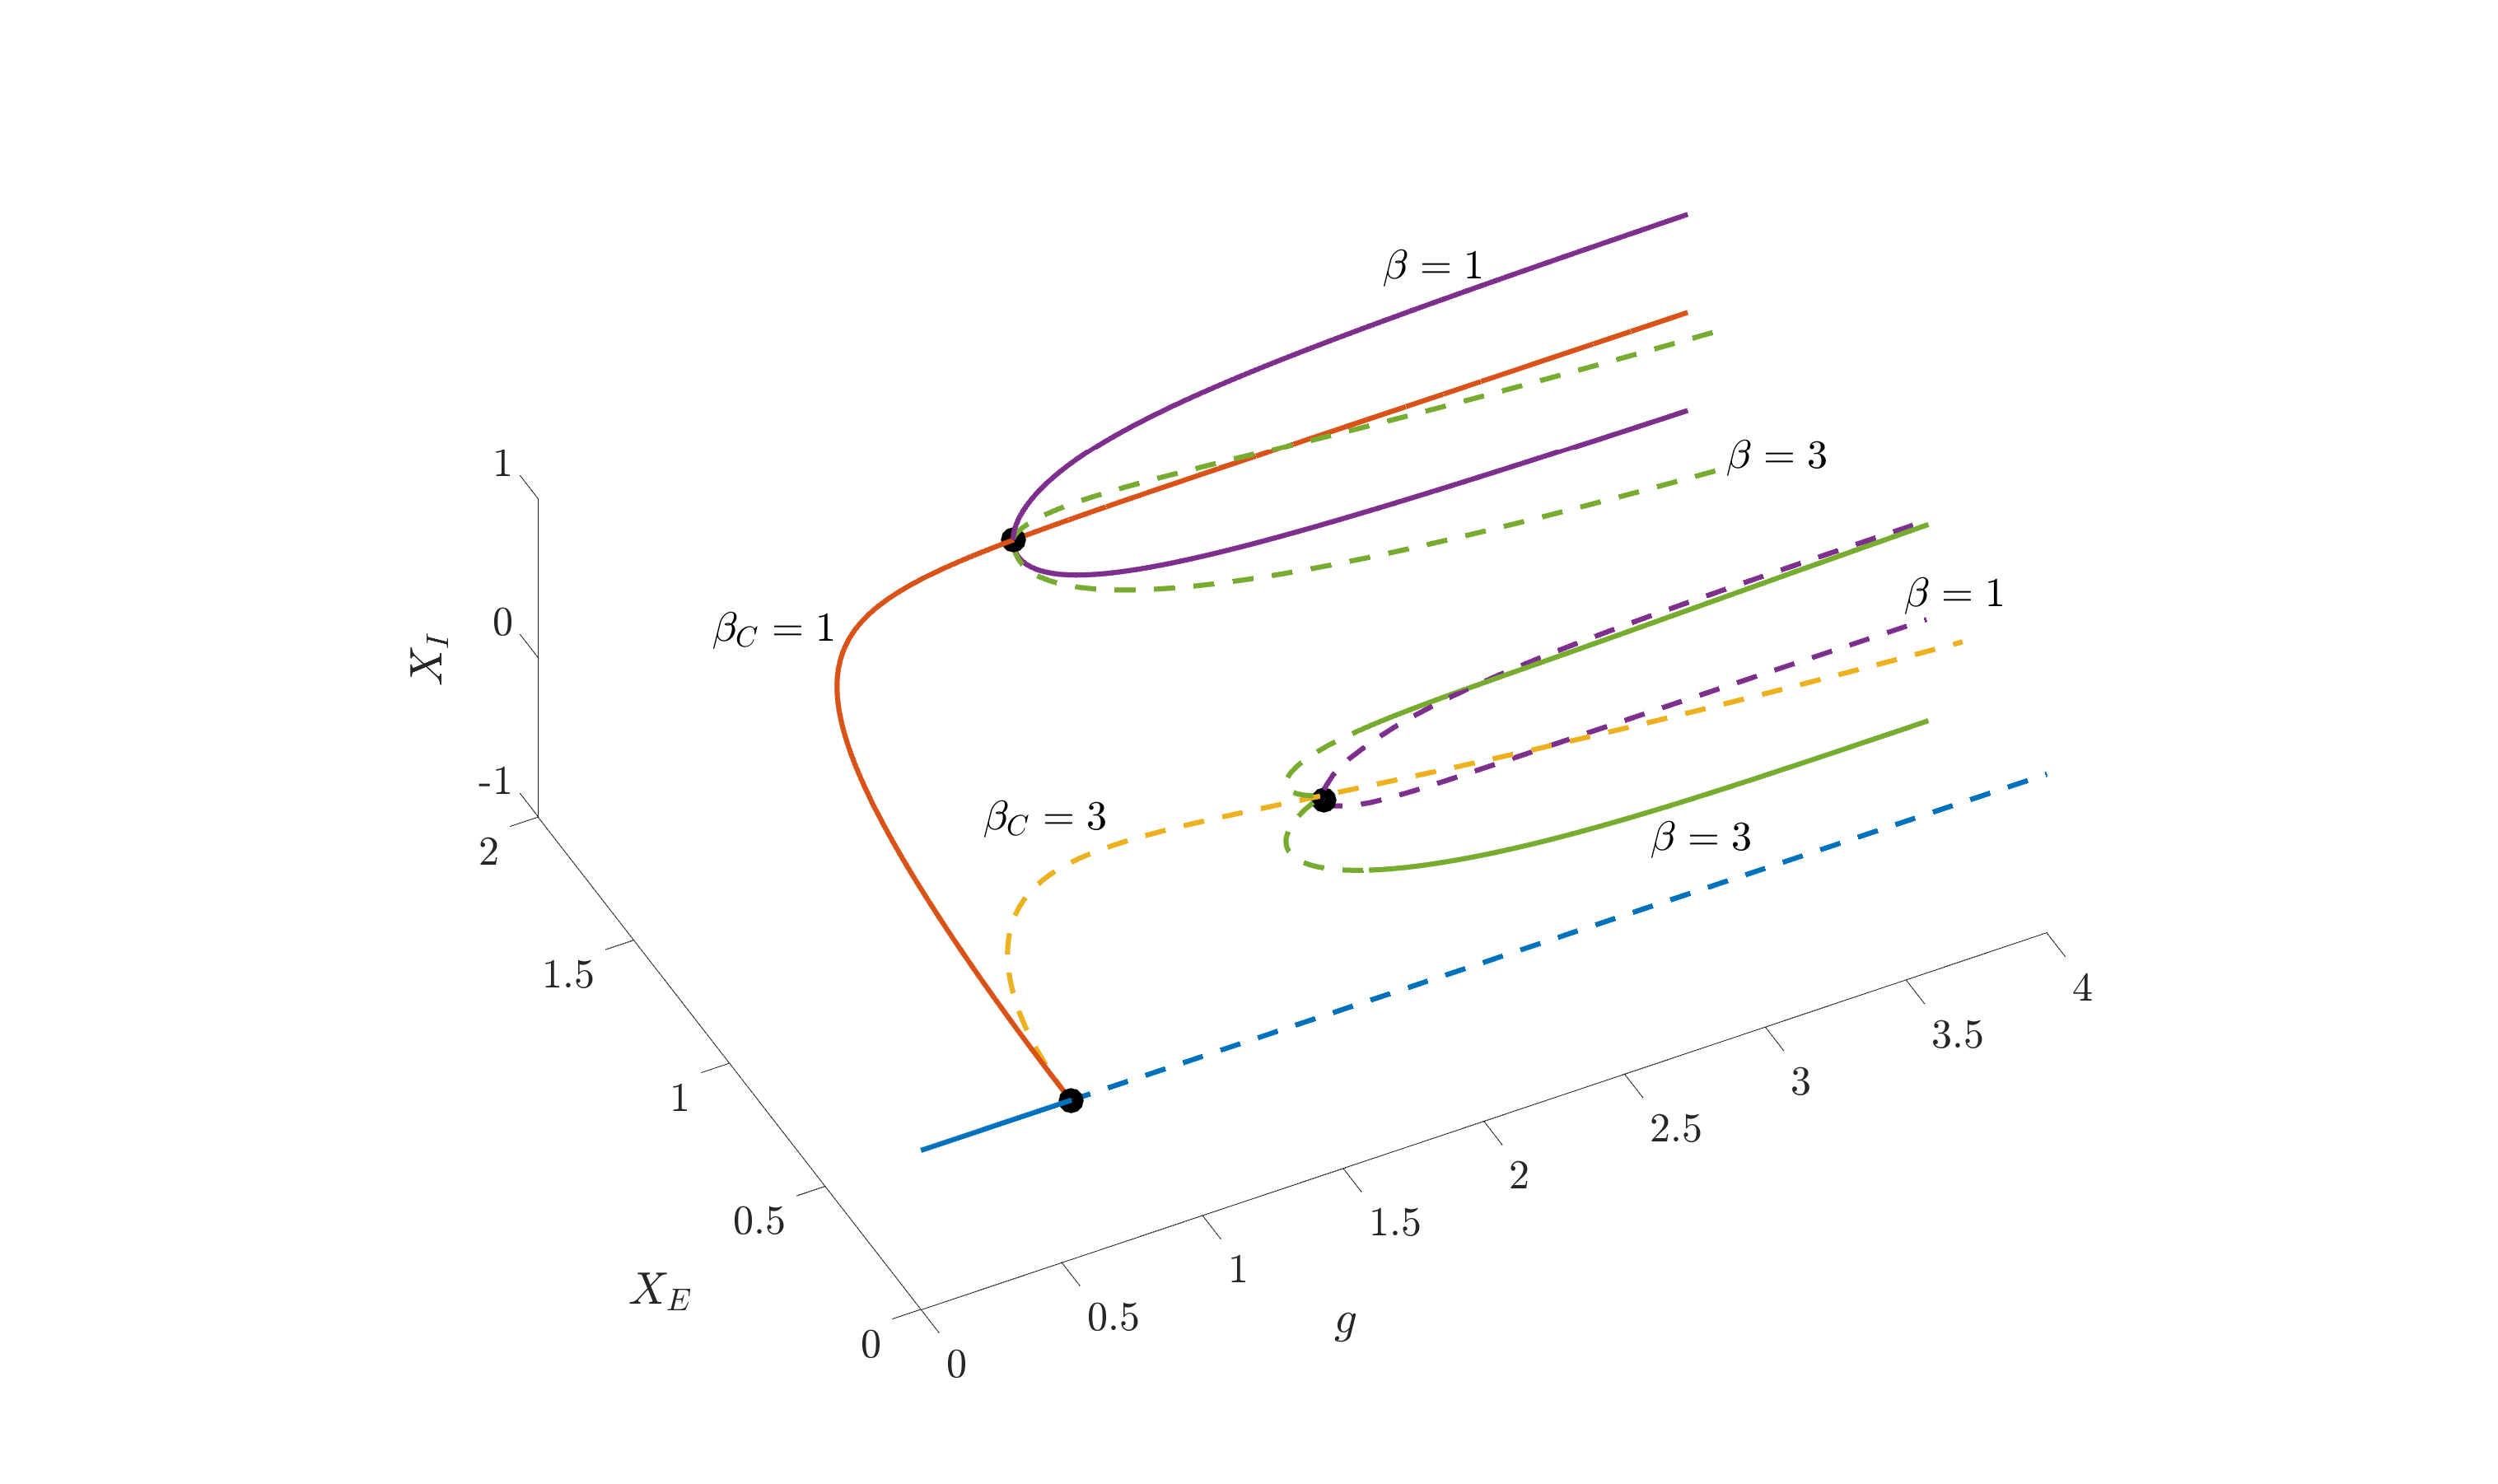
\includegraphics[width=16cm]{images/bdclusters20c43D.eps} 
    % 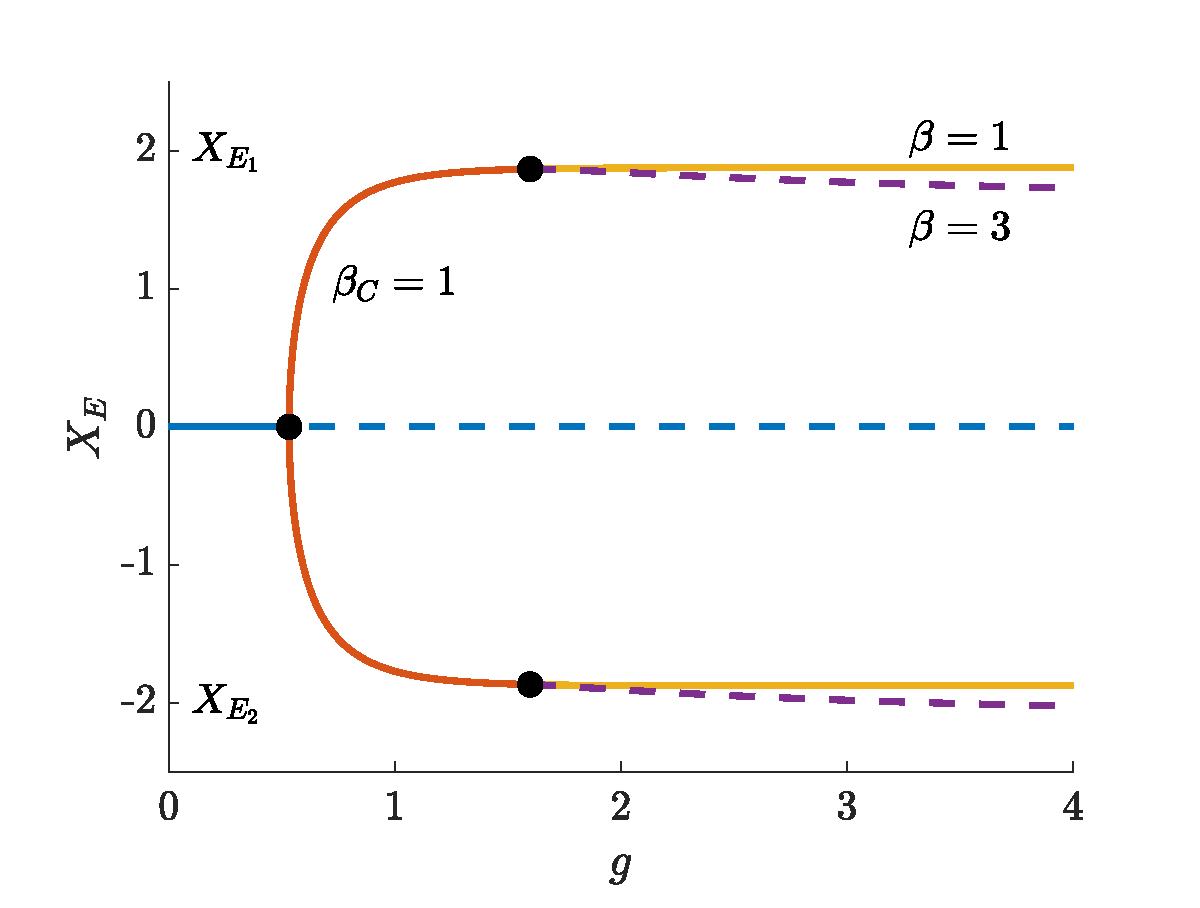
\includegraphics[width=8cm]{images/bdclusters20c4Ebetac1.eps} &
    % 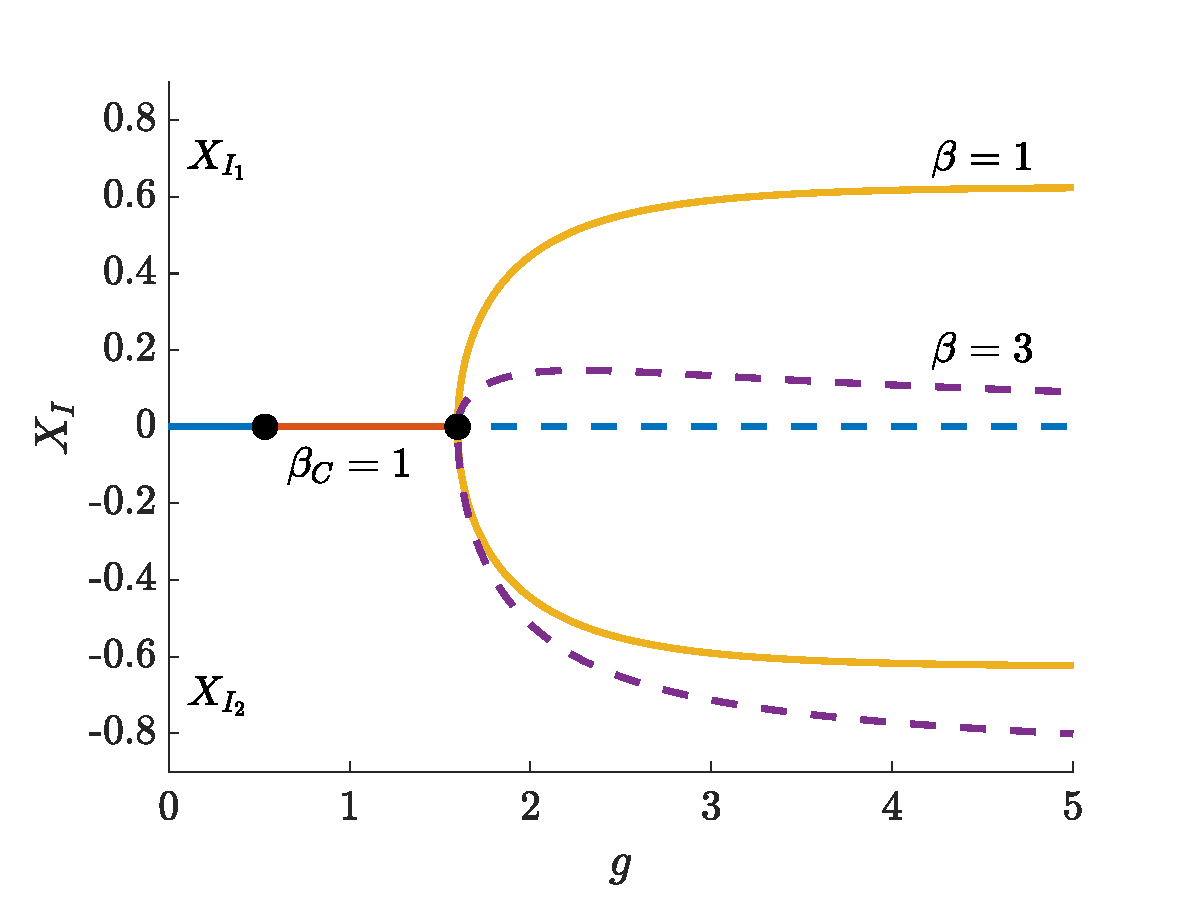
\includegraphics[width=8cm]{images/bdclusters20c4Ibetac1.eps} \\
    % 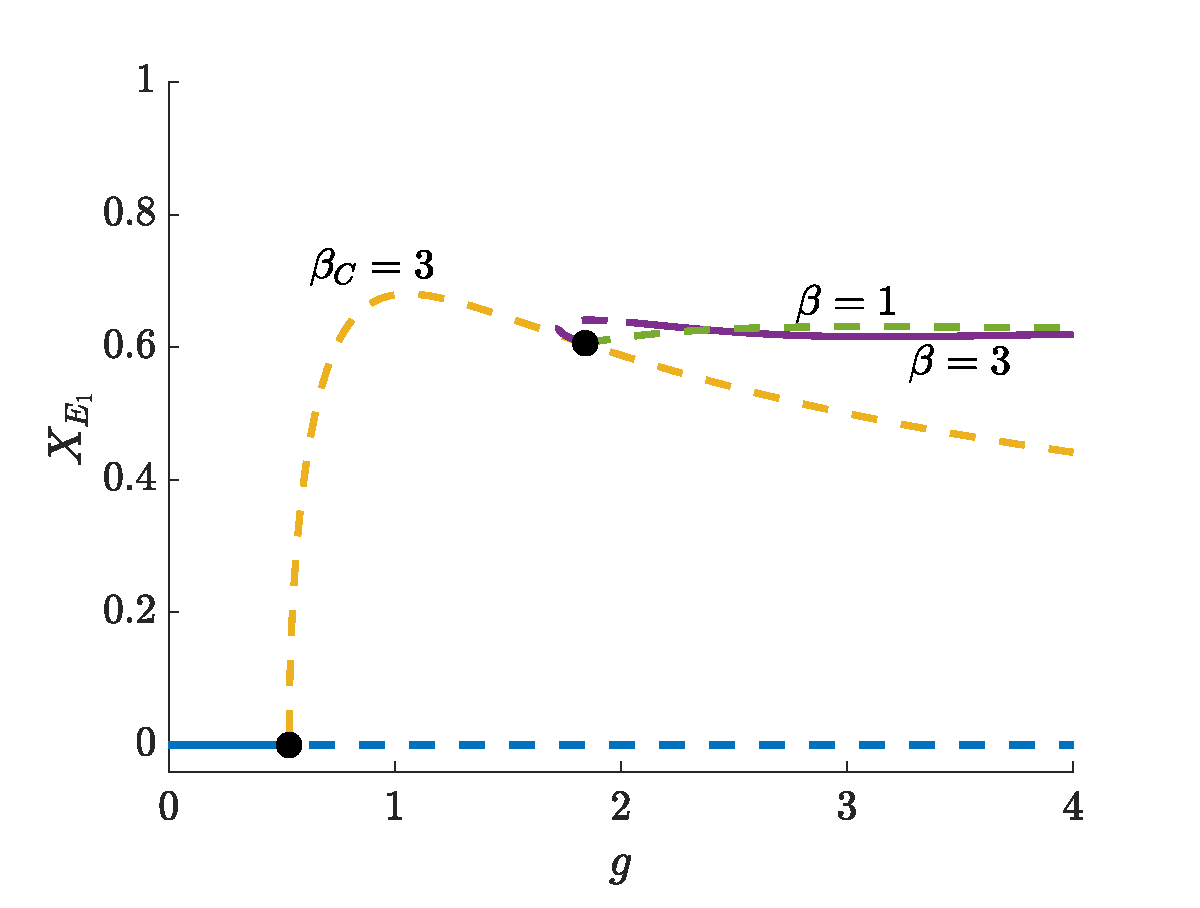
\includegraphics[width=8cm]{images/bdclusters20c4Ebetac3.eps} &
    % 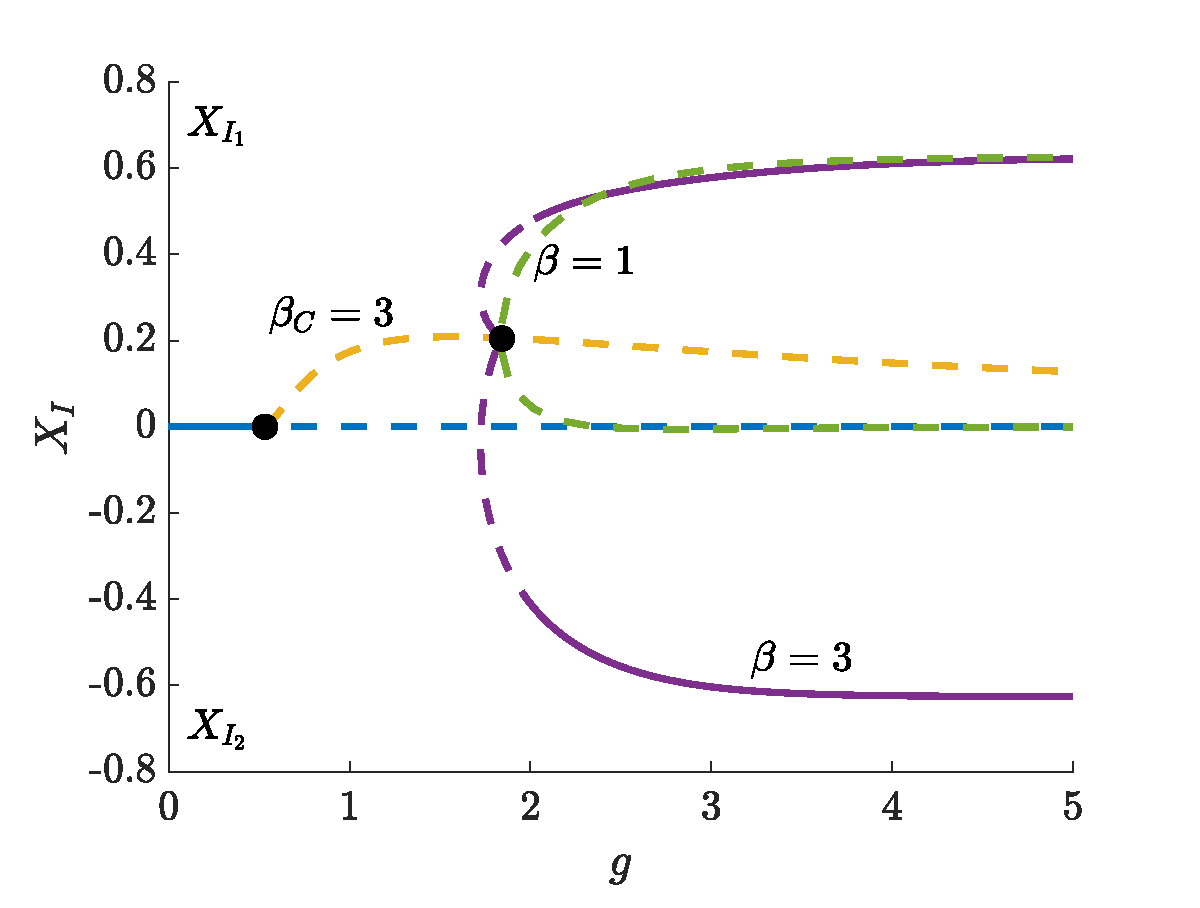
\includegraphics[width=8cm]{images/bdclusters20c4Ibetac3.eps}
    % \end{tabular}
    \caption{Top panel shows $C_1/C_2$ branches of equilibria of \cref{eqn:sys_Basic} with excitatory clustering for all valid values of $\beta_C$, i.e. $\beta_C =1$ and $\beta_C=3$. Symmetric pitchfork bifurcations at $g = g_C$ and along the $C_1/C_2$ branches indicated with filled circle. (No $I_1/I_2$ branches after symmetric pitchfork bifurcation on $C_1/C_2$ branch are shown to avoid clutter). Middle panel shows $I_1/I_2$ branches bifurcating from $\beta_C = 1$ branch. Bottom panel shows $I_1/I_2$ branches bifurcating from $C_1/C_2$ branches (only $x_{E_1}$ is shown to avoid clutter). Stable fixed points are indicated with solid lines. $N = 20$, $n_C = 4$, $p = 4$, $n_I = 4$, $\alpha = 4$, $\mu_{EE} = 0.7$.}
    \label{fig:clusterBD1}
\end{figure}

\subsection{Stability and bifurcations along \texorpdfstring{$C_1/C_2$}{C1/C2} branch}

We now analyze the stability of the $C_1/C_2$ branches for $g$ close to $g_C$. Choose any $\beta_C \geq 1$, so that $n_{E_1} = \frac{\beta_C}{\beta_C+1}n_C$ and $n_{E_2} = \frac{1}{\beta_C+1}n_C$. Let $\xvec = (x_{E_1}, x_{E_2}, x_{I})$ be a solution to \cref{eq:cluster3system}. We look at the linearization $D\tilde{F}(\xvec^*)$, where $\xvec^* = (x_{E_1}, \dots, x_{E_1}, x_{E_2}, \dots, x_{E_1}, x_{I}, \dots, x_{I})^T$, where $x_{E_1}$ and $x_{E_2}$ are repeated $n_{C_1}$ and $n_{C_2}$ times, respectively, and $x_I$ is repeated $n_I$ times. Stability will depend on the eigenvalues of $\tilde{H}(\xvec^*)$. A cartoon showing the location of these eigenvalues is given in \cref{fig:HstareigEcluster}. 

\begin{figure}
    \centering
    % \begin{tabular}{ccc}
    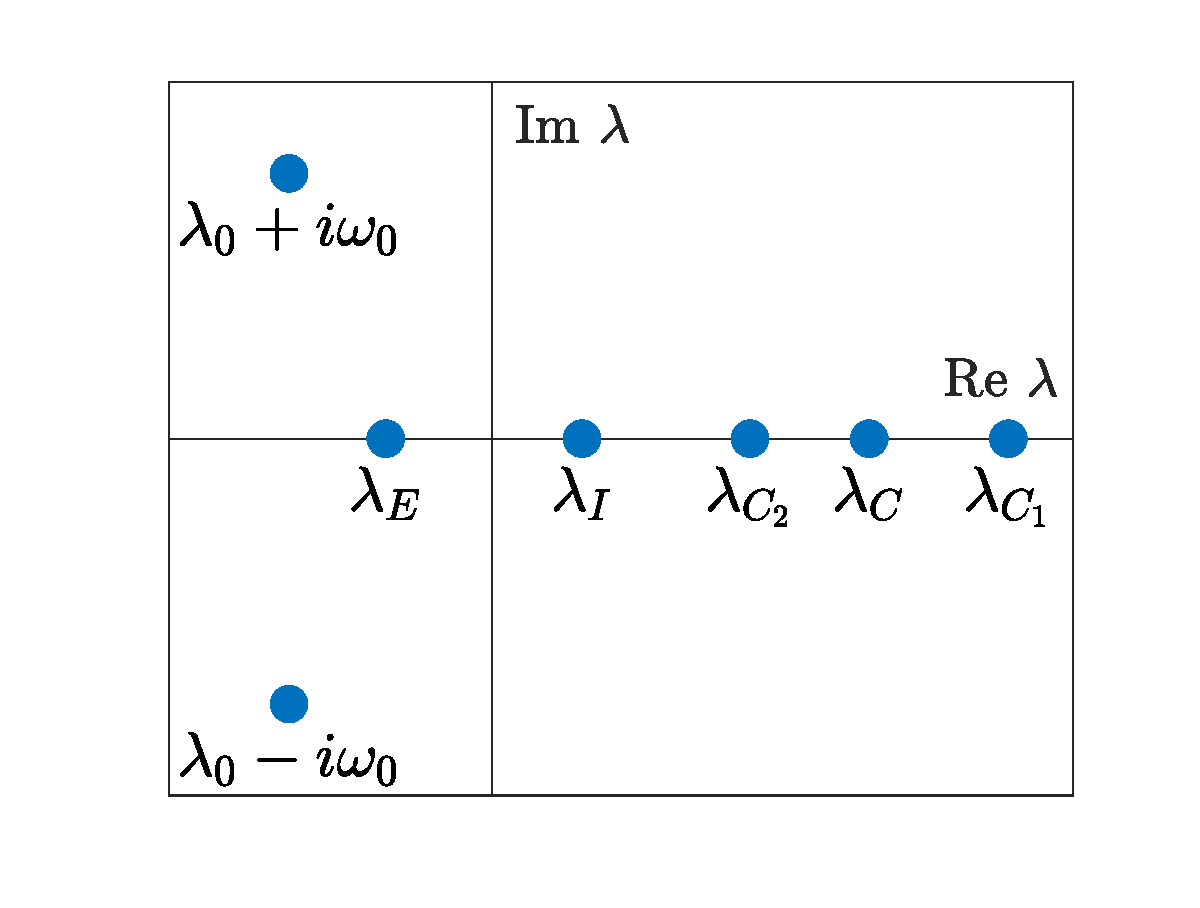
\includegraphics[width=5.7cm]{images/eigpatternxstarEcluster.eps}
    % \end{tabular}
    \caption{Eigenvalue pattern of connectivity matrix $H(\xvec^*)$ for fixed point $\xvec^*$ on $C_1/C_2$ branch with $\beta_C > 1$. The notation for the eigenvalues is explained below.}
    \label{fig:HstareigEcluster}
\end{figure}


We follow the same procedure as with the $I_1/I_2$ branches in the previous section.  First, we linearize the reduced system \cref{eq:cluster3system} about $(x_{E_1}, x_{E_2}, x_{I})$ to get the Jacobian
\[
J_3(\xvec) = \frac{g}{\sqrt{N}} H_3(\xvec) - I_3,
\]
where 
\begin{equation}\label{eq:H3C}
H_3(\xvec) = \mu
\begin{bmatrix} 
    (p-1)n_C \sech^2(g x_{E_1}) & 0 & -p n_C \sech^2(g x_{I}) \\
    0  & (p-1)n_C \sech^2(g x_{E_2}) & -p n_C \sech^2(g x_{I}) \\
    p n_C \frac{\beta_C}{\beta_C+1} \sech^2(g x_{E_1}) &
    p n_C \frac{1}{\beta_C+1} \sech^2(g x_{E_2}) &
    -(p n_C - \alpha) \sech^2(g x_{I})
 \end{bmatrix}
\end{equation}
and $I_3$ is the $3 \times 3$ identity matrix. We have the following proposition concerning the eigenvalues of $H_3(\xvec)$ and $\tilde{H}(\xvec^*)$. The proof is omitted since it is similar to that of \cref{prop:H3eig}.

\begin{proposition}\label{prop:H3Ceig}
Let $\xvec = (x_{E_1}, x_{E_2}, x_{I})$ be a solution to \cref{eq:cluster3system} and $\xvec^*$ the corresponding fixed point of \cref{eq:reducedmatrixform}, and let $H_3(\xvec)$ and $\tilde{H}(\xvec^*)$ be defined by \cref{eq:H3C} and \cref{eq:tildeHxstar}. Then
\begin{compactenum}[(i)]
    \item Every eigenvalue of $H_3(\xvec)$ is an eigenvalue of $\tilde{H}(\xvec^*)$.
    \item $\tilde{H}(\xvec^*)$ has the following additional eigenvalues:
    \begin{itemize}
        \item $\lambda_{C_1} := (p-1) n_C \mu \sech^2(g x_{E_1})$ with multiplicity $n_{C_1} - 1$.
        \item $\lambda_{C_2} := (p-1) n_C \mu \sech^2(g x_{E_2})$ with multiplicity $n_{C_2} - 1$.
        \item $\lambda_{I} := \alpha \mu \sech^2(g x_{I})$ with multiplicity $n_{I} - 1$.
    \end{itemize}
\end{compactenum}
\end{proposition}

Using \cref{eq:XE1E2asymp} and \cref{eq:XE1} and simplifying, the corresponding eigenvalues of $D\tilde{F}(\xvec^*)$ are located, to leading order, at
\begin{equation}\label{eq:DFclustereigs}
\begin{aligned}
\lambda_{C_1}^*(g) &= \frac{g-g_C}{g} \left( 1 - \frac{3}{1-\beta_C+\beta_C^2 }\right) \\
\lambda_{C_2}^*(g) &= \frac{g-g_C}{g} \left( 1 - \frac{3 \beta_C^3}{1-\beta_C+\beta_C^2 }\right) \\
\lambda_{I}^*(g) &= \frac{\alpha \mu g}{\sqrt{N}} - 1
\end{aligned}
\end{equation}
for $g$ close to $g_C$. As in the previous section, $\lambda_{C_1}^*(g)$ is negative for $1 \leq \beta_C < 2$ and positive for $\beta > 2$; $\lambda_{C_2}(g)$ is negative for $\beta_C  > 1/2$; and $\lambda_{I}(g)$ is negative for all $\beta_C$ for $N$ sufficiently large. These imply that the $C_1/C_2$ branch is initially unstable for $\beta_C > 2$ (see \cref{fig:clusterBD1} and \cref{fig:clusterBD2}). For $N = 100$ and $n_C = 10$, it is interesting that while the $C_1/C_2$ branches corresponding to $\beta_C = 4$ and $\beta_C = 9$ in \cref{fig:clusterBD2} are initially unstable, they become stable at a value of $g > g_C$ which is indicated with a diamond on the plot. At this point, the $n_{C_1}$ eigenvalues corresponding to $\lambda_{C_1}$ cross through the origin on the real axis from positive to negative. As $g$ is further increased, these branches lose stability at the symmetric pitchfork bifurcation point. This phenomenon is not observed for $N=20$ and $n_C=4$ (\cref{fig:clusterBD1}).

It remains to find leading order expressions for the eigenvalues of $H_3(\xvec)$. When $\xvec = 0$, the matrix $H_3(0)$ has a single eigenvalue at $\lambda_C$ and a complex conjugate pair of eigenvalues $\lambda_0 \pm \omega_0$, where these are defined at the beginning of this section. We following the same asymptotic procedure as in the previous section. $H_3(\xvec^*)$ has a real eigenvalue corresponding to $\lambda_C$ located at
\[
\lambda_C(\xvec^*) = (p-1)n_C \mu  \left(1 - (1 - \beta_C+\beta_C^2)g^2 x_{E_1}^2 \right) + \mathcal{O}\left(\frac{1}{N^2} \right).
\]
Substituting the estimate \cref{eq:XE1} for $x_{E_1}$ and simplifying, the eigenvalue $\lambda_C^*(g) $of $J_3(\xvec^*)$ corresponding to $\lambda_C$ is located, to leading order, at 
\begin{align*}
    \lambda_C^*(g) &= -2\left( \frac{g - g_C}{g_C} \right)  && g \geq g_C
\end{align*}
for $g$ close to $g_C$. Since this eigenvalue is always negative, it will not affect stability. Similarly, $H_3(\xvec)$ has a complex conjugate pair of eigenvalues $\lambda_0 + i \omega_0$, where the real part is given by
\begin{equation*}
\lambda_0(g, \beta_C) = \frac{\mu}{2}\left[ (\alpha - n_C) - \beta_C g^2 n_C (p - 1) x_{E_1}^2 \right]
\end{equation*}
to leading order, for $g$ close to $g_C$. Since we are taking $n_C \geq \alpha$, this is always negative for $g$ close to $g_C$. Thus for $g$ close to $g_C$, the $C_1/C_2$ branches are initially stable for $1 \leq \beta_C \leq 2$ and initially unstable for $\beta_C > 2$ (see the top panel of \cref{fig:clusterBD1} as well as \cref{fig:clusterBD2}).

As $g$ is further increased from $g_C$, there is a second symmetric pitchfork bifurcation on each $C_1/C_2$ branch as the eigenvalue $\lambda_I^*(g)$ of $D\tilde{F}(\xvec^*)$ crosses the origin (see \cref{fig:clusterBD1} and \cref{fig:clusterBD2}). The behavior at this symmetric pitchfork bifurcation is the same as in the previous section. There is an $I_1/I_2$ branch of solutions for every possible division of the inhibitory cells into exactly two clusters. We can characterize these branches using the parameter $\beta = n_{I_1}/n_{I_2}$, as we did in the previous section. When $\beta_C = 1$, $x_I = 0$, and this bifurcation takes place at 
\begin{equation}\label{eq:gpitchinhbeta1}
g_I = \frac{\sqrt{N}}{\alpha \mu}.
\end{equation}
For $\beta_C > 1$, this bifurcation takes place at $g$ much greater than $g_C$, thus the approximations \cref{eq:XE1E2asymp} and \cref{eq:XE1} do not hold. To locate these bifurcations, we will examine the behavior of the system as $g$ becomes large.

\subsection{\texorpdfstring{$C_1/C_2$}{C1/C2} branches for large \texorpdfstring{$g$}{g}}

First, we look at the behavior of solutions on the $C_1/C_2$ branch as $g$ becomes large. The large $g$ behavior of the $C_1/C_2$ branches will depend on the ratio $\beta_C = n_{C_1}/n_{C_2}$. When $\beta_C = 1$, $x_{E_2} = -x_{E_1} := x_E$, and $x_I = 0$ for all $g \geq g_C$. Numerical parameter continuation suggests that $x_{E} \rightarrow \hat{x}_{E} > 0$ as $g \rightarrow \infty$, which implies that $\tanh(g x_{E}) \rightarrow 1$. It follows from the first row of \cref{eq:cluster3system} that 
\begin{equation}\label{eq:xEhat}
\hat{x}_{E} = \frac{\mu}{\sqrt{N}}(p-1)n_C.
\end{equation}
For $\beta_C > 1$, numerical parameter continuation suggests $x_I \rightarrow 0$ as $g \rightarrow \infty$, but $\tanh(g x_I) \rightarrow \hat{y}_I \neq 0$. There are two patterns for the limiting behavior on the $C_1/C_2$ branches, which depend on whether $\beta_C < \beta_C^*$ or $\beta_C > \beta_C^*$, where $\beta_C^*$ will be determined below. These are illustrated in \cref{fig:betacstar}.\\
\begin{itemize}
    \item Case 1: for $1 < \beta_C < \beta_C^*$, $x_{E_1} \rightarrow \hat{x}_{E_1} > 0$ and $x_{E_2} \rightarrow \hat{x}_{E_2} < 0$. 
    \item Case 2: for $\beta_C > \beta_C^*$, $x_{E_1} \rightarrow 0$ with $\tanh(g x_{E_1}) \rightarrow \hat{y}_{E_1} \neq 0$, and $x_{E_2} \rightarrow \hat{x}_{E_2} < 0$.\\
\end{itemize}

\begin{figure}
    \centering
    % \begin{tabular}{cc}
    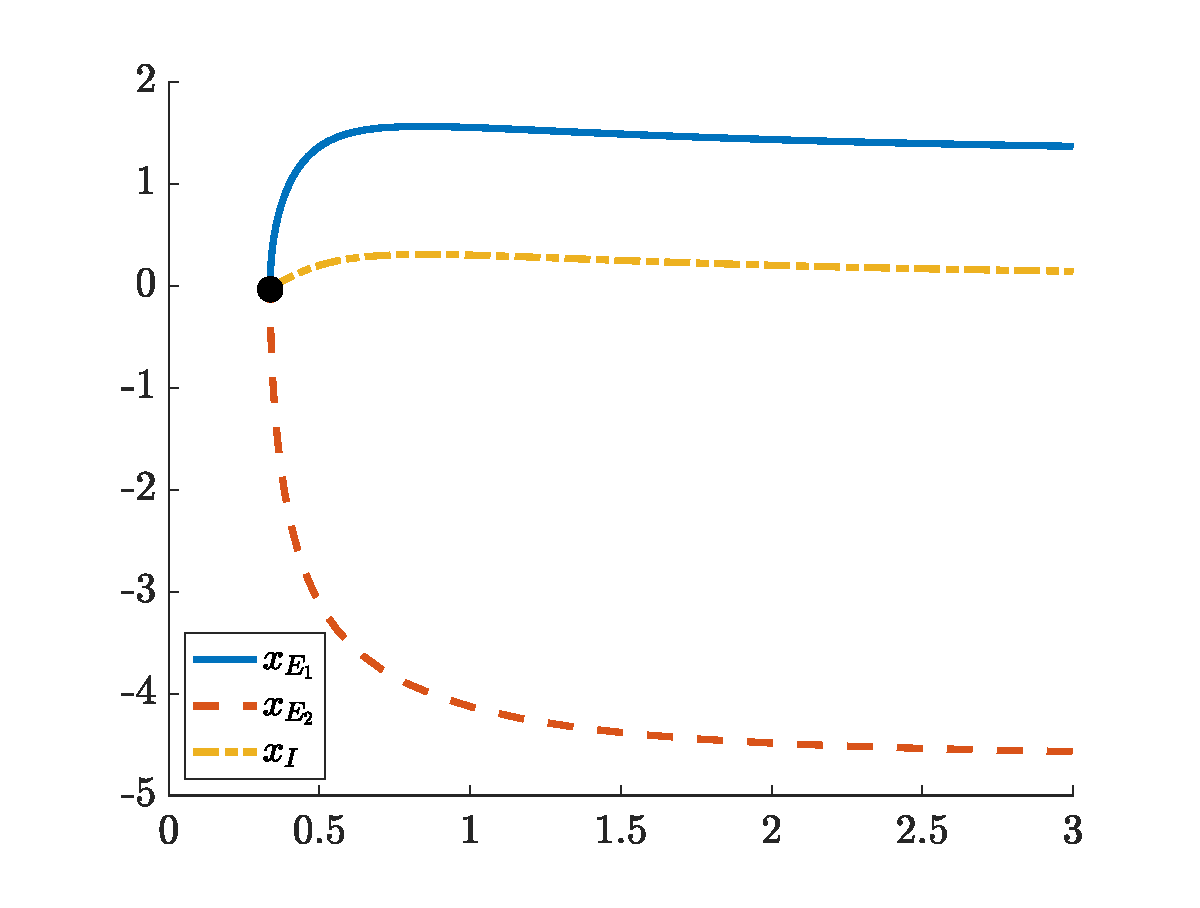
\includegraphics[width=7.8cm]{images/clusterbeforebetacstar.eps}
    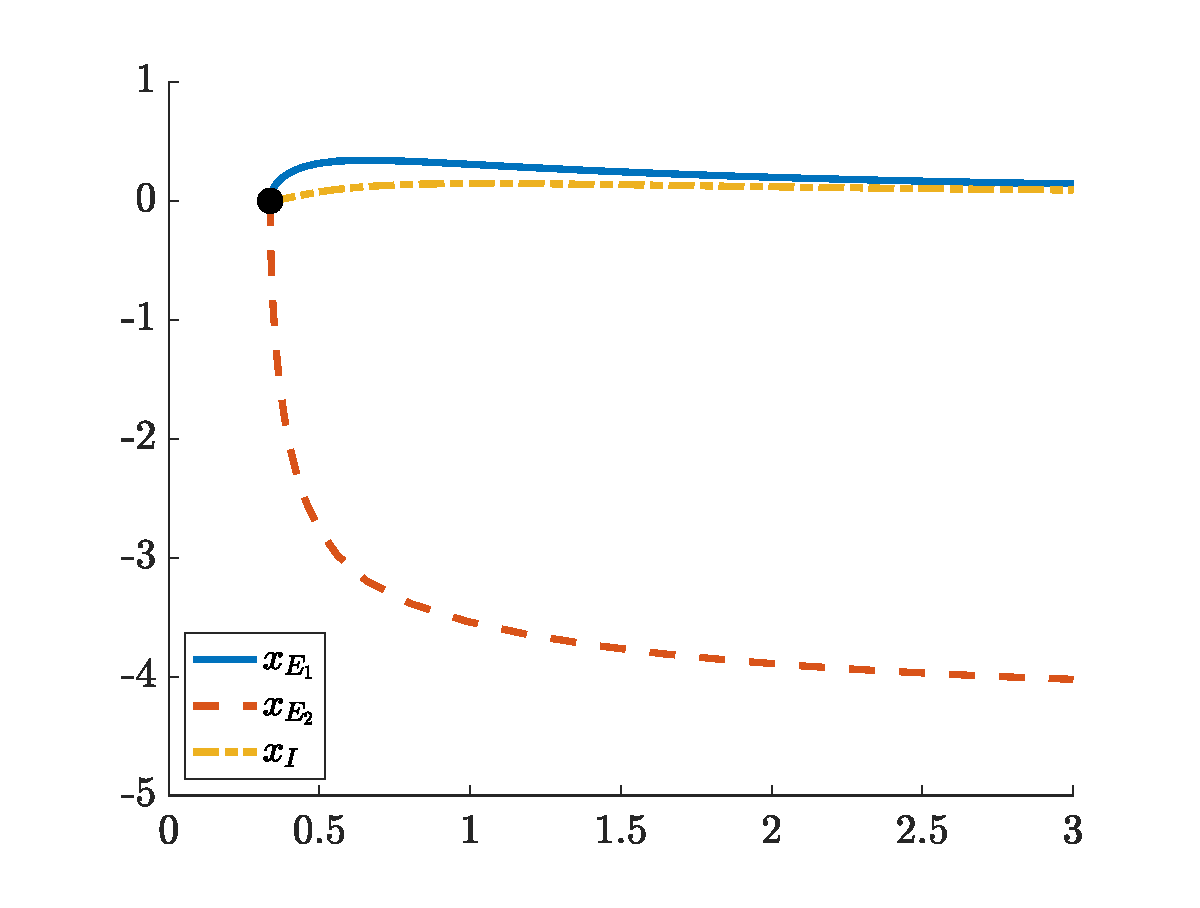
\includegraphics[width=7.8cm]{images/clusterafterbetacstar.eps}
    % \end{tabular}
    \caption{Solutions $x_{E_1}$, $x_{E_2}$, and $x_I$ vs $g$ on $C_1/C_2$ branches for $1 < \beta_C < \beta_C^*$ (left) and $\beta_C > \beta_C^*$ (right). $N = 50$, $n_C = 10$, $p = 4$, $n_I = 10$, $\alpha =4$, $\mu = 0.7$. $\beta_C = 7/3$ (left), and $\beta_C = 9$ (right). $\beta_C^* = 5.15385$.}
    \label{fig:betacstar}
\end{figure}
\noindent For Case 1, since $\tanh(g x_{E_1}) \rightarrow 1$ and $\tanh(g x_{E_2}) \rightarrow -1$, we can solve for $\hat{y}_I$ using row 3 of \cref{eq:cluster3system} to get
\begin{equation}\label{eq:yihat}
    \hat{y}_I = \frac{\beta_C - 1}{\beta_C+1} \frac{p n_C}{p n_C - \alpha},
\end{equation} 
from which it follows that
\begin{equation}\label{eq:xilimiteq}
    x_I \rightarrow \frac{1}{g}\tanh^{-1}\left( \frac{\beta_C - 1}{\beta_C+1} \frac{p n_C}{p n_C - \alpha} \right) \text{ as } g \rightarrow \infty.
\end{equation}
Using \cref{eq:yihat} with rows 1 and 2 of \cref{eq:cluster3system},
\begin{equation}\label{eq:xEhat12}
\begin{aligned}
    \hat{x}_{E_1} &= \frac{\mu}{\sqrt{N}}\left( (p-1)n_C - \frac{\beta_C - 1}{\beta_C+1} \frac{p^2 n_C^2}{p n_C - \alpha} \right) \\
    \hat{x}_{E_2} &= \frac{\mu}{\sqrt{N}}\left( -(p-1)n_C - \frac{\beta_C - 1}{\beta_C+1} \frac{p^2 n_C^2}{p n_C - \alpha} \right),
\end{aligned}
\end{equation}
which reduce to \cref{eq:xEhat} when $\beta_C = 1$. Since $n_C p = f N \rightarrow \infty$ as $N \rightarrow \infty$, this simplifies to
\begin{equation}\label{eq:xEhat12IlargeN}
    \begin{aligned}
        x_{E_1} &\rightarrow\frac{\mu}{\sqrt{N}}\left( (p-1)n_C - \frac{\beta_C - 1}{\beta_C+1} p n_C \right) \\
        x_{E_2} &\rightarrow \frac{\mu}{\sqrt{N}}\left( -(p-1)n_C - \frac{\beta_C - 1}{\beta_C+1} p n_C \right) \\
        x_I &\rightarrow \frac{1}{g}\tanh^{-1}\left( \frac{\beta_C - 1}{\beta_C+1} \right)
    \end{aligned}
\end{equation}
as $g, N \rightarrow \infty$. For \cref{eq:xEhat12} to be valid, the consistency conditions $\hat{x}_{E_1} > 0$ and $\hat{x}_{E_2} < 0$ must be satisfied. Since $\hat{x}_{E_2} < 0$ always holds, \cref{eq:xEhat12} is consistent as long as
\begin{equation}\label{eq:betaCineq}
(p-1)n_C - \frac{\beta_C - 1}{\beta_C+1}\frac{p^2 n_C^2}{p n_C - \alpha}  > 0.
\end{equation}
This reduces to the condition $\beta_C < \beta_C^*$, where
\begin{equation}\label{eq:betaCstar}
    \beta_C^* = \frac{(n_C p - \alpha )(2 p - 1) + \alpha p}{n_C p + \alpha(p-1)}.
\end{equation}
As $N \rightarrow \infty$, the $\alpha$ in the denominator of \cref{eq:betaCineq} becomes insignificant, and we have $\beta_C^* \rightarrow 2 p-1$. This depends on neither $p$ nor $n_C$, since these variables are involved in \cref{eq:betaCineq} only in the form $p n_C = n_E = f N$. We note that the largest possible value of $\beta_C$ is $\beta_C = n_C - 1$, which occurs when $n_{C_1} = n_C - 1$ and $n_{C_2} = 1$. Since $p = f N/n_C$, it follows that if either $n_C$ is held constant or $n_C$ scales as $\sqrt{N}$, $\beta_C < \beta_C^*$ will be always satisfied for sufficiently large $N$.

For Case 2, we can solve for $\hat{y}_{E_1}$ and $\hat{y}_I$ using rows 2 and 3 of \cref{eq:cluster3system} to get
\begin{equation}\label{eq:ye1hatyihat}
    \begin{aligned}
        \hat{y}_{E_1} &= \frac{n_C p^2 }{ \alpha(1+\beta_C)(p-1) + n_C p(1 + \beta_C - p)} \\
        \hat{y}_{I} &= \frac{n_C p(p-1) }{ \alpha(1+\beta_C)(p-1) + n_C p(1 + \beta_C - p)},
    \end{aligned}
\end{equation}
from which it follows that
\begin{equation}
    \begin{aligned}
        x_{E_1} &\rightarrow \frac{1}{g} \tanh^{-1} \left( \frac{n_C p^2 }{ \alpha(1+\beta_C)(p-1) + n_C p(1 + \beta_C - p)}  \right) \\
        x_{E_2} &\rightarrow \frac{\mu}{\sqrt{N}}\left( -(p-1)n_C - \frac{n_C^2 p^2(p-1) }{ \alpha(1+\beta_C)(p-1) + n_C p(1 + \beta_C - p)}\right) \\
        x_{I} &\rightarrow \frac{1}{g} \tanh^{-1} \left(\frac{n_C p(p-1) }{ \alpha(1+\beta_C)(p-1) + n_C p(1 + \beta_C - p)} \right).
    \end{aligned}
\end{equation}
as $g \rightarrow \infty$. We note that for $\beta_C > \beta_C^*$, we cannot take $N \rightarrow \infty$ with $n_C$ held fixed since for sufficiently large $N$ we will always have $\beta_C < \beta_C^*$. 

We can use these formulas to find the location of the symmetric pitchfork bifurcations on the $C_1/C_2$ branches when $\beta_C>1$ and $N$ is large. Since we are taking $N$ large, we can assume $\beta_C < \beta_C^*$, as discussed above. At this bifurcation, the eigenvalue $\lambda_I^*(g)$ of $D\tilde{F}(\xvec^*)$ with multiplicity $n_I-1$ crosses through 0. Using the identity $\sech^2(g x_{I}) = 1 - \tanh^2(g x_{I}) = 1 - \hat{y}_I$ as $g \rightarrow \infty$ together with \cref{eq:yihat}, the symmetric pitchfork bifurcation on the $C_1/C_2$ branch corresponding to $\beta_C > 1$ is located, to leading order, at 
\begin{align}\label{eq:gbetaC}
    g_I(\beta_C) &= \frac{\sqrt{N}}{4 \alpha \mu} \frac{(1 + \beta_C)^2}{\beta_C} % + \mathcal{O}\left(\frac{1}{N^{1/2}}\right)
\end{align}
for $N$ large. When $\beta_C = 1$, this reduces to \cref{eq:gpitchinhbeta1}. See \cref{fig:clusterBD2} and the left panel of \cref{fig:pitcherror} for the location of the symmetric pitchfork branches on the $C_1/C_2$ branches. Numerical simulation validates this formula, and suggests that the error term in \cref{eq:gbetaC} has order $\mathcal{O}(N^{-1/2})$ (\cref{fig:pitcherror}, right panel). We note that for $N$ large, $g_I(\beta_C)$ is quadratic in $\beta_C$, has a local minimum at $\beta_C = 1$, and is increasing for $\beta_C > 1$. We can see in \cref{fig:clusterBD2} and \cref{fig:pitcherror} that the location of the symmetric bifurcation points $g_{\beta_C}$ increases with $\beta_C$.

For sufficiently large $N$, each $C_1/C_2$ branch will be stable immediatly preceding this symmetric pitchfork bifurcation. To see this, we evaluate the remaining eigenvalues of $D\tilde{F}(\xvec^*)$ when $g = g_I(\beta_C)$. As $N \rightarrow \infty$, $g_I(\beta_C) \rightarrow \infty$, thus $\sech(g_I(\beta_C) x_{E_j}) \rightarrow 0$ for $j = 1, 2$. It follows that for $g = g_I(\beta_C)$, $\lambda_{C_j} \rightarrow 0$, thus $\lambda_{C_j}^* \rightarrow -1$. By the same argument, taking $N \rightarrow \infty$ will zero out the first two columns of \cref{eq:H3C} when $g = g_I(\beta_C)$. Thus, in the limit $N \rightarrow \infty$, $H_3(\xvec^*)$ will have a pair of eigenvalues at 0 and an additional eigenvalue at $-(p n_C - \alpha) \sech^2 g x_I \leq 0$. The corresponding eigenvalues of $D\tilde{F}(\xvec^*)$ will be negative. In \cref{fig:clusterBD2}, for $N = 100$, the $C_1/C_2$ branches for $\beta_C = 7/3$, 4, and 9 start unstable, but regain stability before the pitchfork bifurcation point. This does not occur for small value of $N$ (see \cref{fig:clusterBD1} for $N=20$).

\begin{figure}
    \centering
    % \begin{tabular}{cc}
    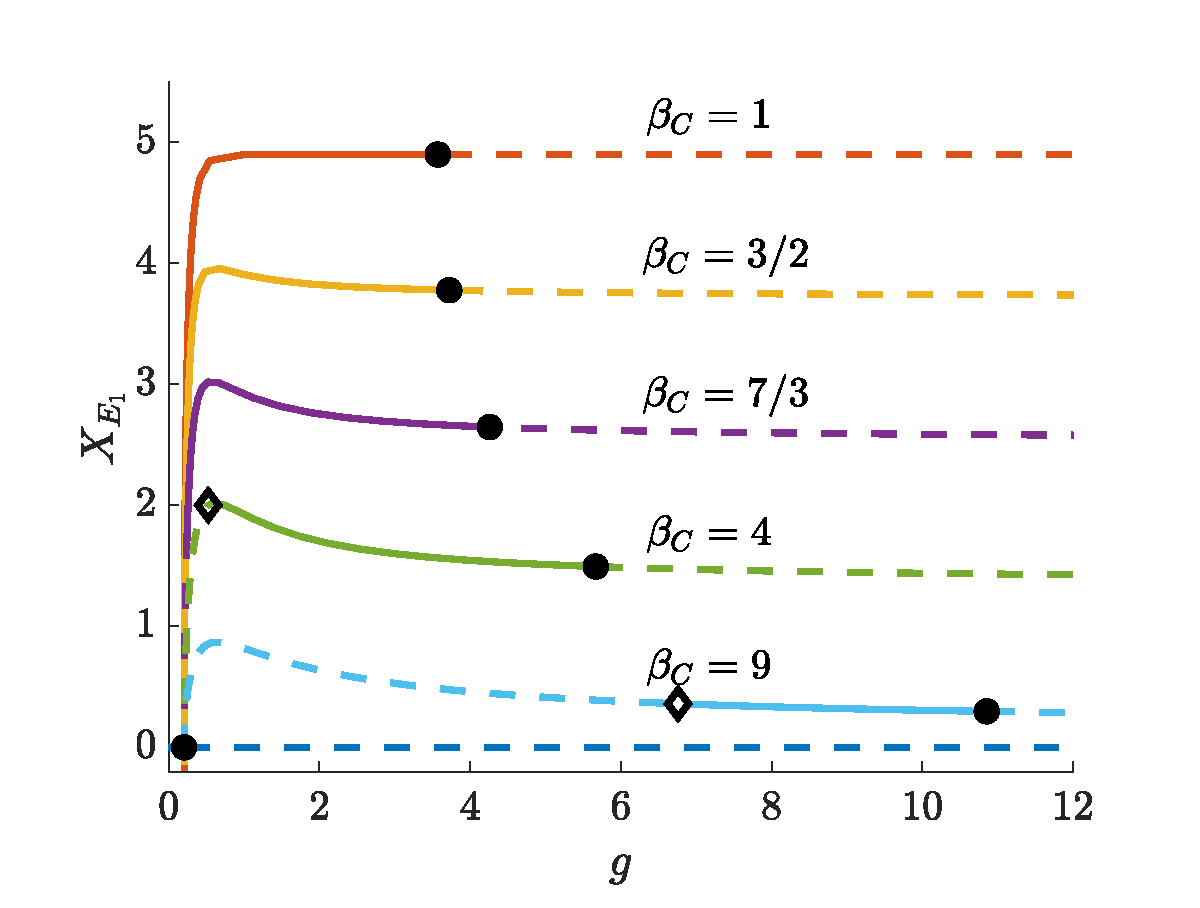
\includegraphics[width=7.8cm]{images/bdclusters100c10E.eps}
    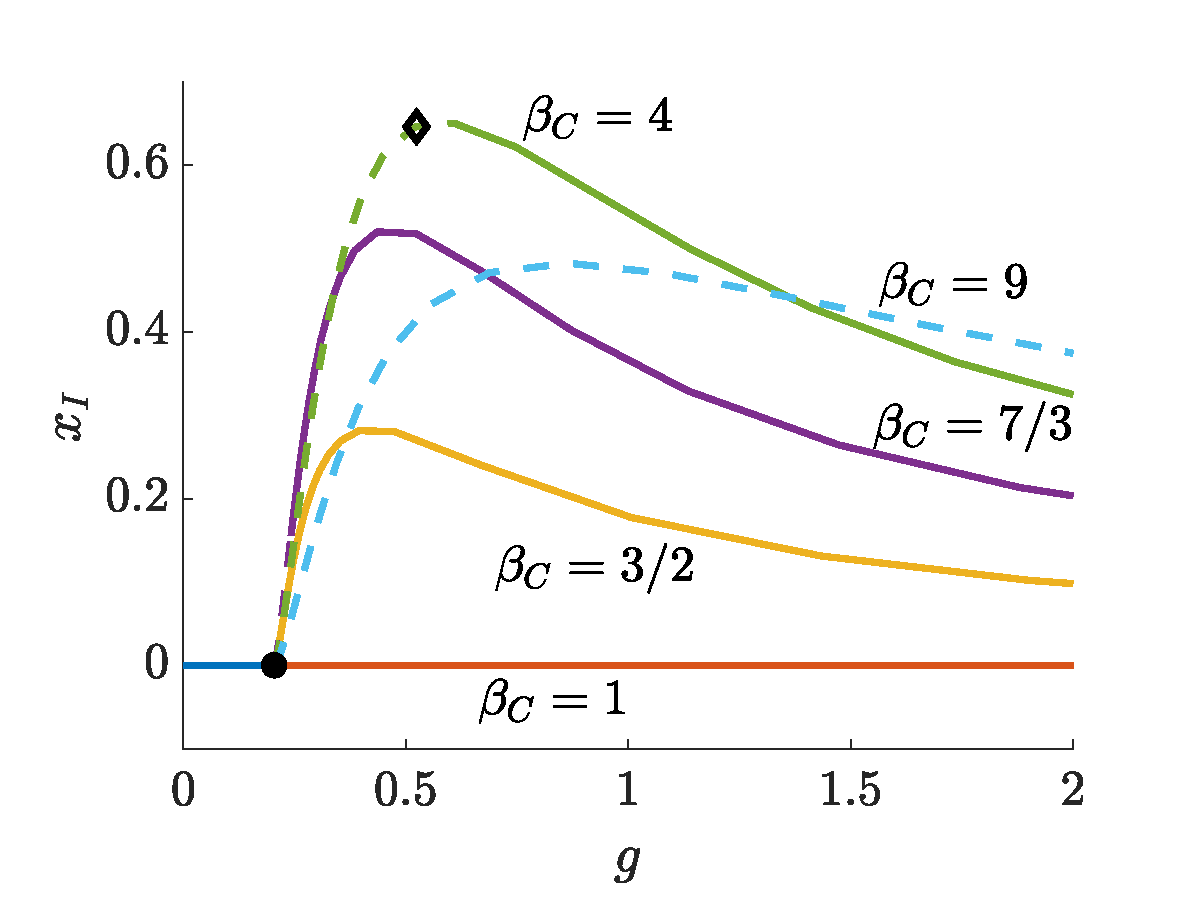
\includegraphics[width=7.8cm]{images/bdclusters100c10Izoom.eps} 
    % 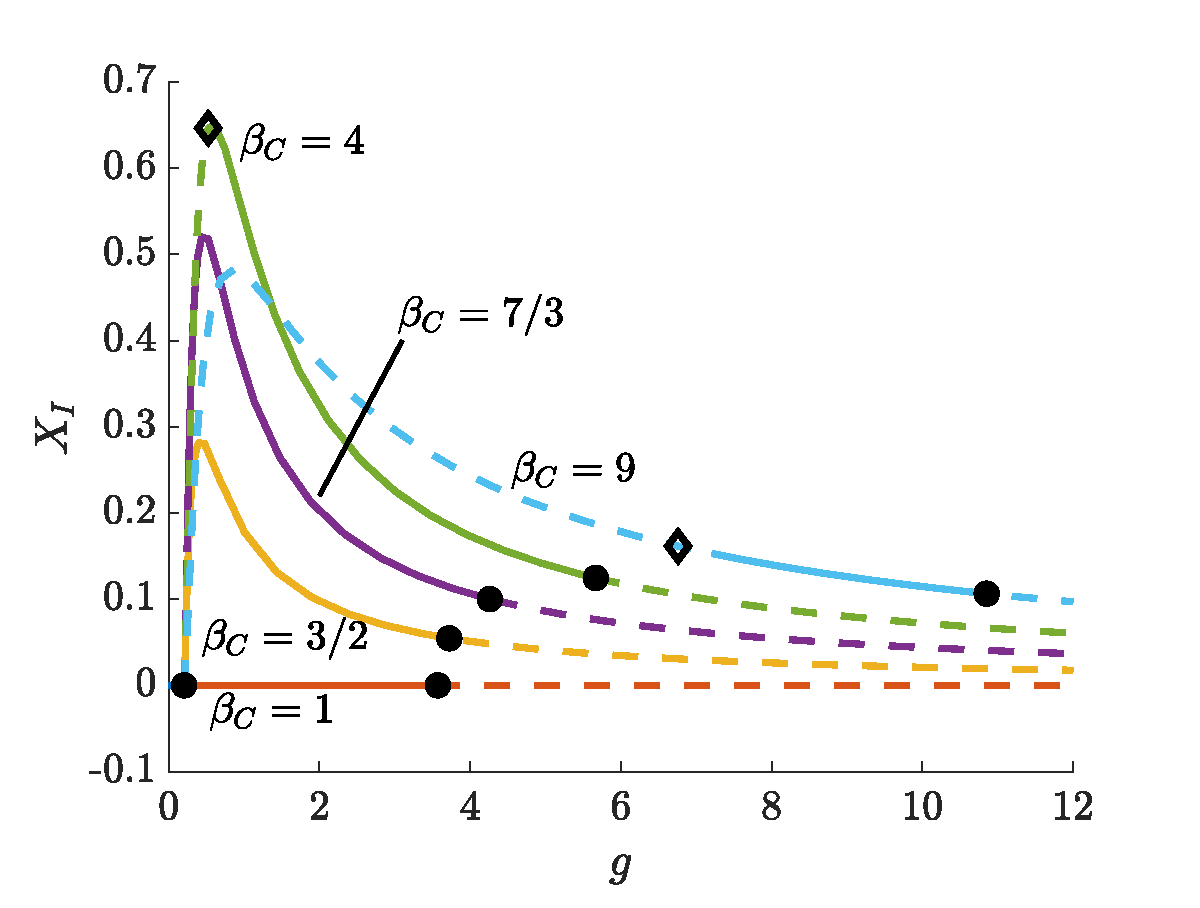
\includegraphics[width=7.8cm]{images/bdclusters100c10I.eps} \\
    \vspace{-1cm}
    % 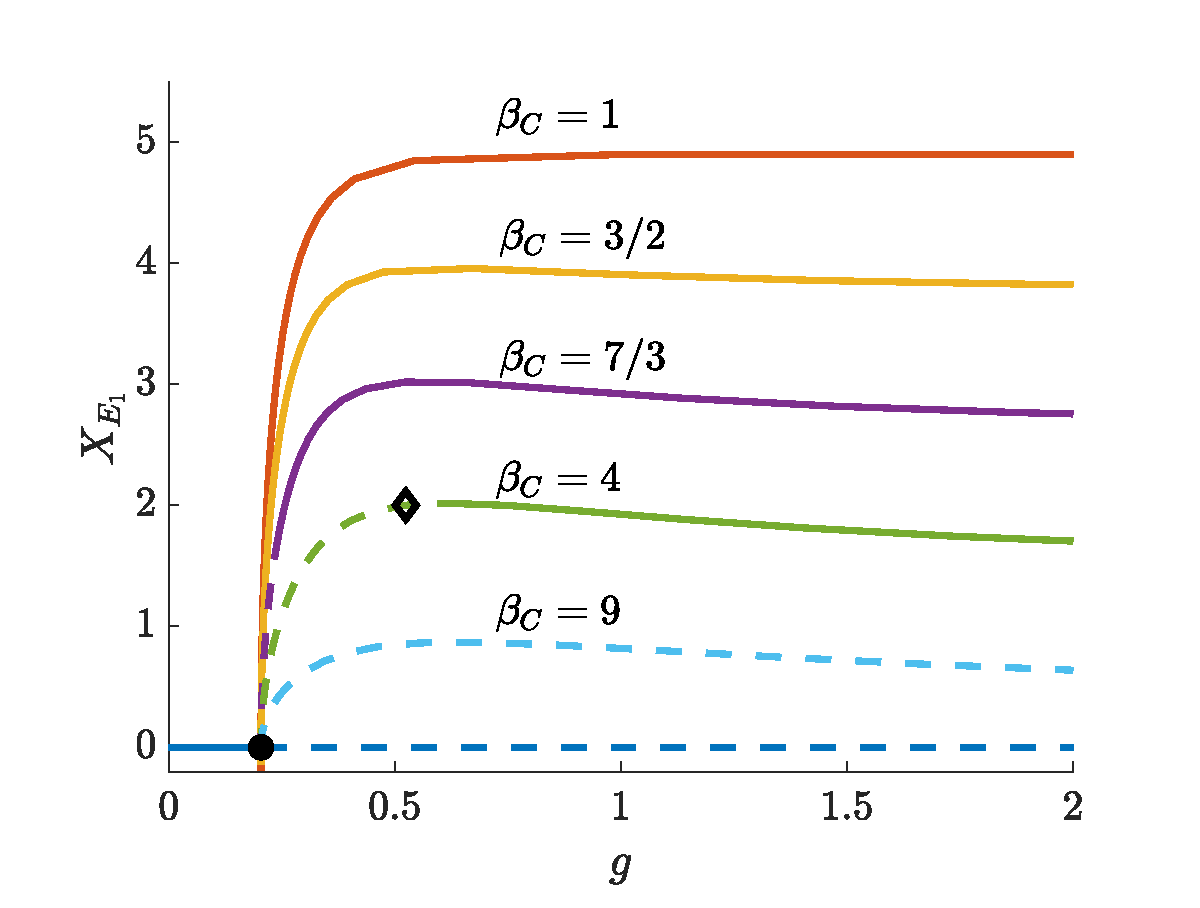
\includegraphics[width=7.8cm]{images/bdclusters100c10Ezoom.eps} &
    % 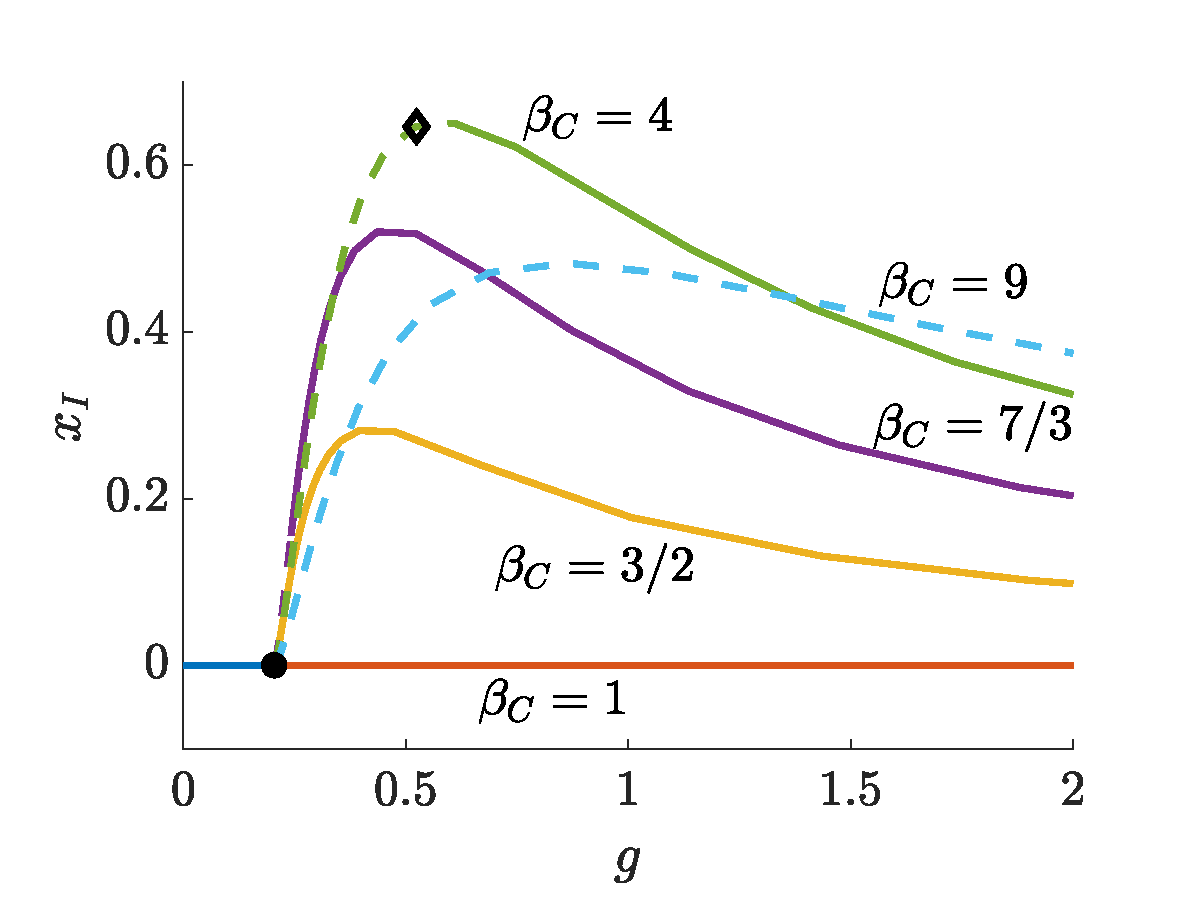
\includegraphics[width=7.8cm]{images/bdclusters100c10Izoom.eps} 
    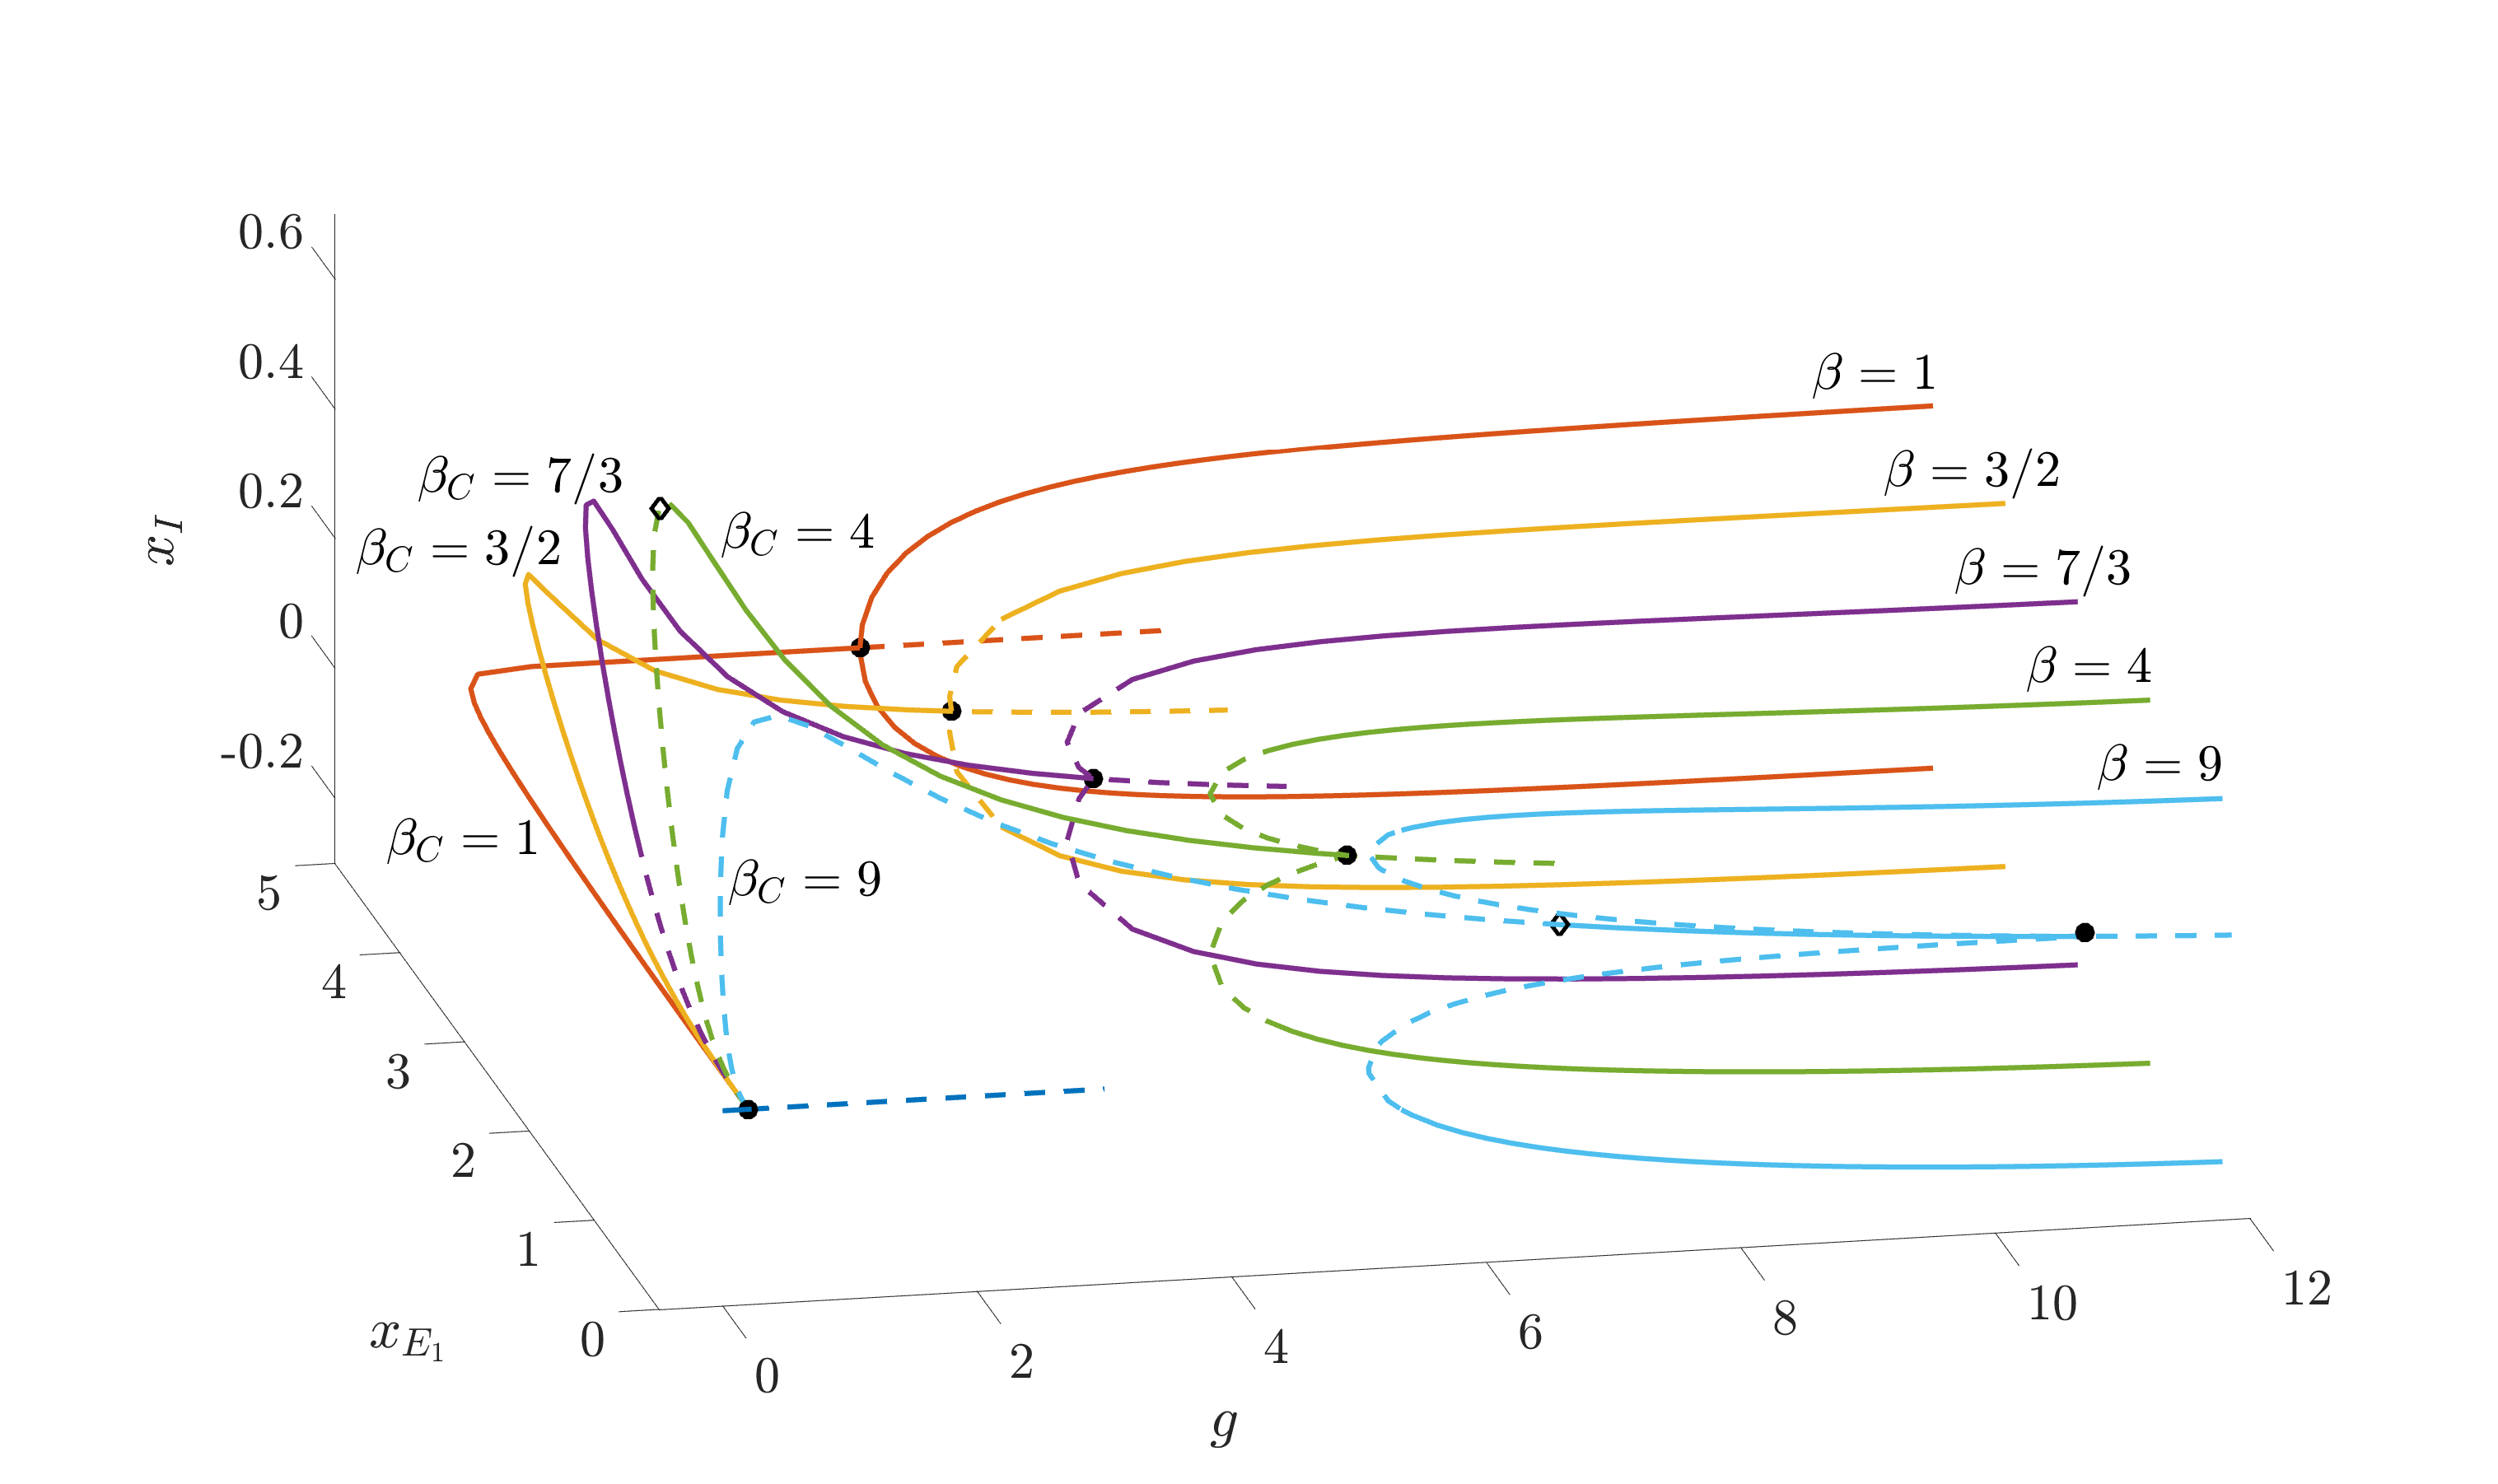
\includegraphics[width=16.5cm]{images/bdclusters100c103D.eps}
    % \end{tabular}
    \caption{Top panel shows $C_1/C_2$ branches of equilibria of \cref{eqn:sys_Basic} with excitatory clustering for all valid values of $\beta_C$. Top left plots $x_{E_1}$ vs $g$. Top right plots $x_I$ vs $g$, zoomed into a narrower range of $g$ to show stability of $C_1/C_2$ branches near $g = g_C$. Symmetric pitchfork bifurcations at $g = g_C$ and along the $C_1/C_2$ branches indicated with filled circle. No branches are shown after these bifurcations to avoid clutter. Bottom panel shows $I_1/I_2$ branches bifurcating from $C_1/C_2$ branches at the symmetric pitchfork bifurcation point. The only $I_1/I_2$ branches shown here is the ones which are eventually stable, which in this case are those with $\beta = \beta_C$. Stable fixed points indicated with solid line, unstable fixed points indicated with dashed line. Unstable $C_1/C_2$ branches for $\beta_C = 4$ and $\beta_C = 9$ become stable at the points indicated with the diamond. $N = 100$, $n_C = 10$, $p = 8$, $n_I = 20$, $\alpha = 4$, $\mu_{EE} = 0.7$.}
    \label{fig:clusterBD2}
\end{figure}

\begin{figure}
    \centering
    \begin{tabular}{cc}
    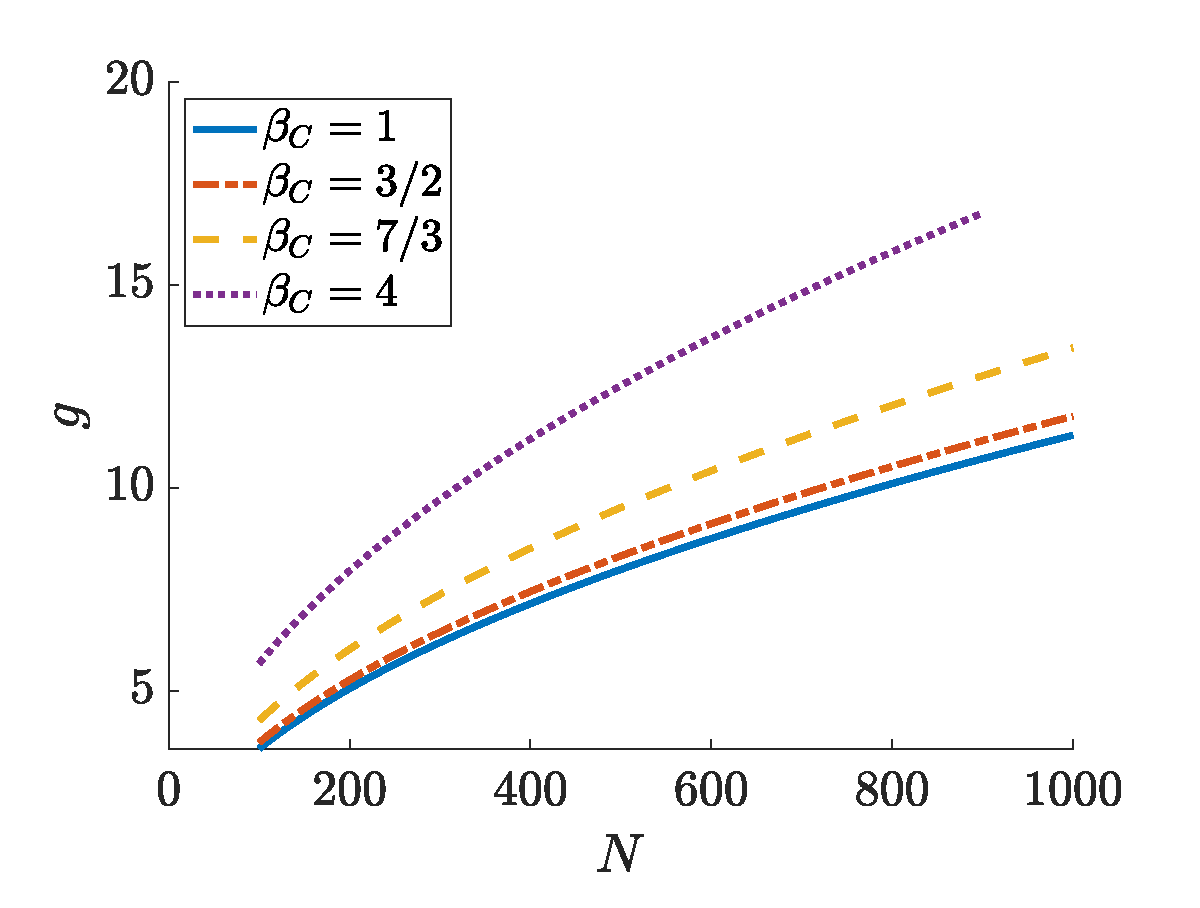
\includegraphics[width=7.8cm]{images/clusterpitchgvsN.eps}
    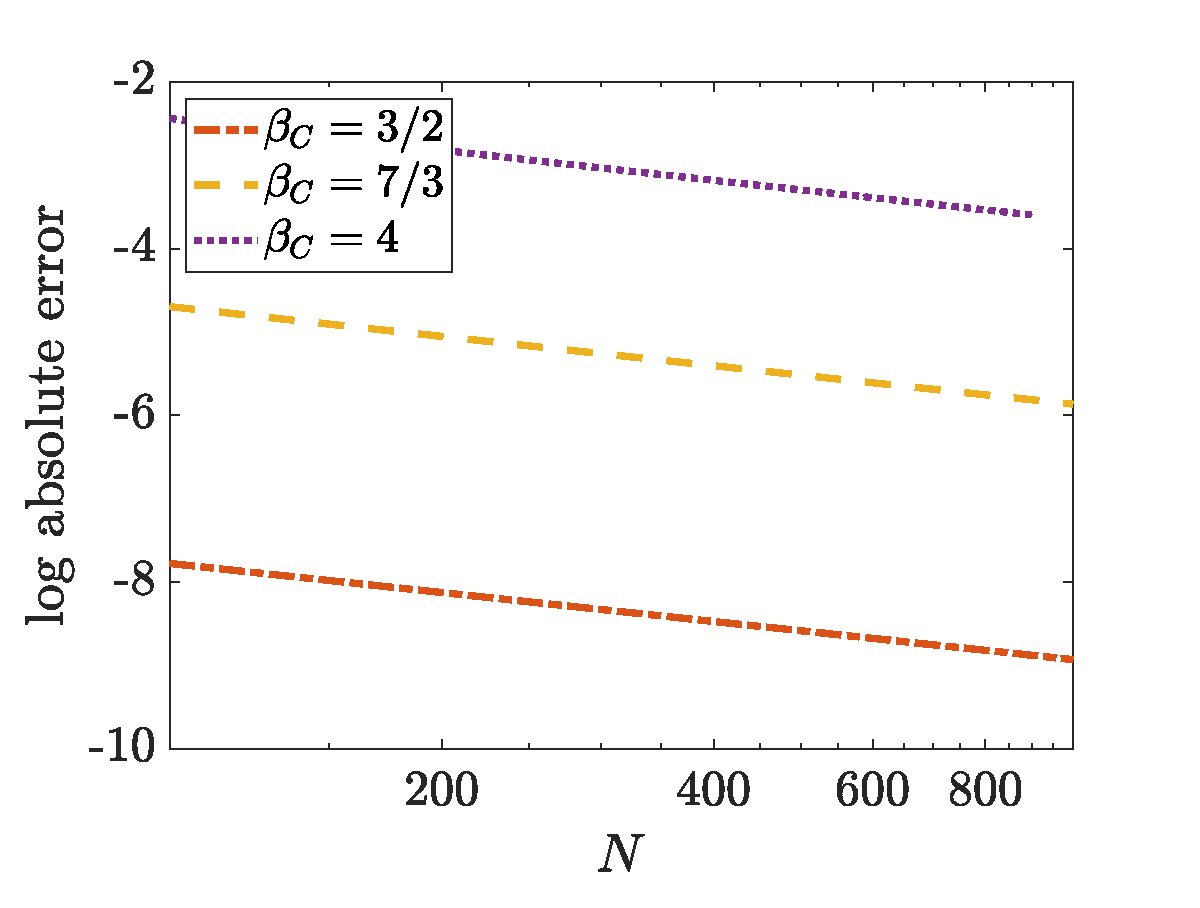
\includegraphics[width=7.8cm]{images/pitcherrorsemilog.eps}
    \end{tabular}
    \caption{Left panel plots location in $g$ of symmetric pitchfork bifurcation point on $C_1/C_2$ branches vs $N$ for various $\beta_C$. Right panel is semi-log plot of log of the absolute error of approximation \cref{eq:gbetaC} vs $N$ for various $\beta_C$. Slope of line is approximately -0.5 for all three $\beta_C$. $n_C = 10$, $\alpha = 4$, $\mu = 0.7$.}
    \label{fig:pitcherror}
\end{figure}

\subsection{Stable fixed points for large \texorpdfstring{$g$}{g}}

After the symmetric pitchfork bifurcation point on the $C_1/C_2$ branches, both the excitatory clusters and inhibitory cells have split into two populations. We are interested in stable fixed points when $g$ is large. In particular, we seek fixed point branches in which the excitatory clusters are split into two populations with ratio $\beta_C = n_{C_1}/n_{C_2}$ and the inhibitory cells are also split into two populations with ratio $\beta = n_{I_1}/n_{I_2}$. This reduces \cref{eqn:sys_Basic} to the system of equations
\begin{equation}\label{eq:cluster4system}
    \begin{aligned}
    \begin{bmatrix} x_{E_1} \\ x_{E_2} \\ x_{I_1} \\ x_{I_2} \end{bmatrix} 
    &= \frac{\mu}{\sqrt{N}} 
    \begin{bmatrix} 
       (p-1)n_C & 0 & -\alpha \frac{\beta}{\beta+1}n_I &  -\alpha \frac{1}{\beta+1}n_I \\
       0  & (p-1)n_C & -\alpha \frac{\beta}{\beta+1}n_I &  -\alpha \frac{1}{\beta+1}n_I \\
       p n_C \frac{\beta_C}{\beta_C+1} &
       p n_C \frac{1}{\beta_C+1} &
       -\alpha \left(\frac{\beta}{\beta+1}n_I-1\right) &  -\alpha \frac{1}{\beta+1}n_I \\
       p n_C \frac{\beta_C}{\beta_C+1} &
       p n_C \frac{1}{\beta_C+1} &
       -\alpha \frac{\beta}{\beta+1}n_I & -\alpha \left(\frac{1}{\beta+1}n_I - 1 \right)
    \end{bmatrix}
    \begin{bmatrix} \tanh(g x_{E_1}) \\ \tanh ( g x_{E_2} ) \\\tanh(g x_{I_1}) \\\tanh(g x_{I_2})  \end{bmatrix},
    \end{aligned}
\end{equation}
Furthermore, numerical parameter continuation suggests that as $g \rightarrow \infty$, $(x_{E_1}, x_{E_2}, x_{I_1}, x_{I_1}) \rightarrow (\hat{x}_{E_1}, \hat{x}_{E_2}, \hat{x}_{I_1}, \hat{x}_{I_2})$, where $\hat{x}_{E_1}, \hat{x}_{I_1} > 0$ and $\hat{x}_{E_2}, \hat{x}_{I_2} < 0$. Using this as an ansatz, equation \cref{eq:cluster4system} reduces to 
\begin{equation}\label{eq:xhat}
    \begin{aligned}
        \hat{x}_{E_1} &= \frac{\mu}{\sqrt{N}}\left[ (p-1)n_C - \alpha \frac{\beta-1}{\beta+1}n_I \right] \\
        \hat{x}_{E_2} &= \frac{\mu}{\sqrt{N}}\left[ -(p-1)n_C - \alpha \frac{\beta-1}{\beta+1}n_I \right] \\
        \hat{x}_{I_1} &= \frac{\mu}{\sqrt{N}}\left[  \frac{\beta_C-1}{\beta_C+1} p n_C - \alpha \left( \frac{\beta-1}{\beta+1}n_I - 1 \right) \right] \\
        \hat{x}_{I_2} &= \frac{\mu}{\sqrt{N}}\left[  \frac{\beta_C-1}{\beta_C+1} p n_C - \alpha \left( \frac{\beta-1}{\beta+1}n_I + 1 \right) \right],
    \end{aligned}
\end{equation}
since $\tanh(g x_{E_1}), \tanh(g x_{I_1}) \rightarrow 1$ and $\tanh(g x_{E_2}), \tanh(g x_{I_2}) \rightarrow -1$ as $g \rightarrow \infty$. Equation \cref{eq:xhat} gives the limiting solutions $(\hat{x}_{E_1}, \hat{x}_{E_2}, \hat{x}_{I_1}, \hat{x}_{I_1})$ as long as the consistency conditions $\hat{x}_{E_1}, \hat{x}_{I_1} > 0$ and $\hat{x}_{E_2}, \hat{x}_{I_2} < 0$ are satisfied. Since $\mu > 0$, the consistency conditions reduce to
\begin{equation}\label{eq:consistency}
    \begin{aligned}
        &(p-1)n_C - \alpha \frac{\beta-1}{\beta+1}n_I > 0 \\
        -&(p-1)n_C - \alpha \frac{\beta-1}{\beta+1}n_I < 0 \\
        &\frac{\beta_C-1}{\beta_C+1} p n_C - \alpha \left( \frac{\beta-1}{\beta+1}n_I - 1 \right) > 0 \\
        &\frac{\beta_C-1}{\beta_C+1} p n_C - \alpha \left( \frac{\beta-1}{\beta+1}n_I + 1 \right) < 0.
    \end{aligned}
\end{equation}
The first pair of inequalities in \cref{eq:consistency} is satisfied if and only if
\[
    \left| \frac{\beta-1}{\beta+1} \right| < \frac{(p-1)n_C}{\alpha n_I} = 1 - \frac{1}{p},
\]
where we used the fact that $n_C p = n_E = \alpha n_I$. Since we are taking $\beta \geq 1$, this simplifies to 
\begin{equation}\label{eq:betacond}
    1 \leq \beta < 2p-1
\end{equation}
Similarly, the second pair of inequalities in \cref{eq:consistency} is satisfied if and only if 
\[
    \alpha \left( \frac{\beta-1}{\beta+1}n_I - 1 \right) < \frac{\beta_C-1}{\beta_C+1} p n_C < \alpha \left( \frac{\beta-1}{\beta+1}n_I + 1 \right),
\]
which simplifies to 
\begin{equation}\label{eq:bccondition}
    \frac{2 \beta n_I - \beta - 1}{2 n_I + \beta + 1} < \beta_C < \frac{2 \beta n_I + \beta + 1}{2 n_I - \beta - 1}.
\end{equation}
A list of all valid pairs of $(\beta, \beta_C)$ for some small values of $N$ is given in \cref{table:validbeta}. If $n_C = n_I$, it follows from \cref{eq:bccondition} that 
\[
n_{I_1} - \frac{1}{2} < n_{C_1} < n_{I_1} + \frac{1}{2}.
\]
Since $n_{C_1}$ must be an integer, $n_{C_1} = n_{I_1}$, which implies $\beta_C = \beta$. We note that the fixed point $\xvec^*$ corresponding to each of these $(\beta, \beta_C)$ is eventually stable for sufficiently large $g$, since as $g\rightarrow \infty$, $H(\xvec^*)$ approaches the $\Zerovec$ matrix, thus the Jacobian approaches $-I$, which has a single eigenvalue of $-1$ with multiplicity $N$. The solutions corresponding to the top row of \cref{table:validbeta} are shown in the bottom panel of \cref{fig:clusterBD1}, and the solutions corresponding to the bottom row are shown in the bottom panel of \cref{fig:clusterBD2}; we can see from the figures that the corresponding fixed points are all stable for sufficiently large $g$.

\begin{table}
\centering
    \begin{tabular}{lllll}
        \toprule
        $N$ & $n_I$ & $n_C$ & $p$ & $(\beta, \beta_C)$ \\
        \midrule
        20 & 4 & 4 & 4 & (1, 1), (3, 3) \\
        25 & 5 & 5 & 4 & (3/2, 3/2), (4, 4) \\
        25 & 5 & 4 & 5 & (4, 3) \\
        35 & 7 & 7 & 4 & (4/3, 4/3), (5/2, 5/2), (6, 6) \\
        35 & 7 & 4 & 7 & (5/2, 3) \\
        50 & 10 & 10 & 4 & (1, 1), (3/2, 3/2), (7/3, 7/3), (4, 4) \\
        100 & 20 & 10 & 8 & (1, 1), (3/2, 3/2), (7/3, 7/3), (4, 4), (9, 9) \\
        \bottomrule
    \end{tabular}
    \vspace{0.25cm}
    \caption{Valid pairs $(\beta, \beta_C)$ for selected small values of $N$. $\alpha = 4$ in all cases.}
    \label{table:validbeta}
\end{table}

\subsection{Excitatory clusters with weight parameters unchanged}

We can also choose the weights as in the unclustered case, i.e. $\mu_{EI} = -\alpha \mu_{EE}$, $\mu_{II} = -\alpha \mu_{EE}$, and $\mu_{IE} = \mu_{EE}$. In this case, the two eigenvalues of $H$ with positive real part are $\lambda_I = \alpha \mu_{EE}$ and $\lambda_C = (p-1)\mu_{EE}$. If $\lambda_C > \lambda_I$, which occurs when $n_C < \frac{f N}{\alpha+1}$, the behavior is qualitatively the same as for the case balanced weight parameters discussed above. If  $\lambda_C < \lambda_I$, which occurs when $n_C > \frac{f N}{\alpha+1}$, the order of the two symmetric pitchfork bifurcations is reversed. As $g$ is increased, the inhibitory cells bifurcate from the origin first, followed by the excitatory clusters.

\subsection{Restored self-coupling}
We can restore self-coupling of neurons with each excitatory cluster by replacing the matrix $\Kvec_{p}$ in \cref{eq:Hcluster} with the $p\times p$ matrix consisting of all 1s. The effect of this in the reduced model \cref{eq:reducedmatrixform} is to replace the matrix $(p-1) \mu_{EE} I_{n_C}$ in the upper left block of \cref{eq:tildeH} with $p \mu_{EE} I_{n_C}$. The eigenvalues of $H$ are then given by:
\begin{itemize}
\item $\lambda_I := \alpha \mu > 0$ with multiplicity $n_I - 1$
\item $\lambda_E := 0$ with multiplicity $(p-1) \times n_C = n_E - n_C$.
\item $\lambda_C := p n_C \mu > 0$, with multiplicity $n_C - 1$.
\item A complex conjugate pair of eigenvalues $\lambda_0 \pm i \omega_0$, with 
\begin{equation*}
    \lambda_0 := \frac{1}{2}\mu \alpha, \quad 
    \omega_0 := \frac{1}{2}\mu \sqrt{ \alpha( 4 n_C p - \alpha ) },
\end{equation*}
\end{itemize}
The eigenvalue pattern is similar to that in the middle panel of \cref{fig:Heigpattern}, except the complex conjugate pair $\lambda_0 \pm i \omega_0$ has positive real part. As a consequence, there will be a Hopf bifurcation at the origin at $g_H = \sqrt{N}/\alpha \mu$. Parameter continuation with AUTO indicates that the resulting limit cycle has all excitatory clusters synchronized and all inhibitory cells synchronized, and is unstable for all $g > g_H$. In addition, timestepping simulations suggest that there are no stable limit cycles for any value of $g$. The pattern of symmetric pitchfork bifurcations, first at the origin and then on each $C_1/C_2$ branch, is the same as for the case with no self-coupling.

\section{Inhibitory clusters}\label{sec:inhibitoryclusters}

We will briefly consider the case where the inhibitory cells are clustered, while the excitatory cells remain unclustered. Suppose the inhibitory cells are grouped into $n_{C_I}$ inhibitory clusters of size $p_I$. For the choice of weights $\mu_{EI} = -\alpha \mu_{EE}$, $\mu_{II} = -\alpha \mu_{EE}$, and $\mu_{IE} = \mu_{EE}$, the eigenvalues of $H$ are:
\begin{itemize}
\item $\lambda_I := \alpha \mu_{EE} > 0$ with multiplicity $(p_I-1) \times n_{C_I} = n_I - n_{C_I}$.
\item $\lambda_E := -\mu_{EE} < 0$ with multiplicity $n_E - 1$.
\item $\lambda_{C_I} := -(p_I-1)\alpha \mu_{EE} < 0$, with multiplicity $n_{C_I}-1$.
\item A complex conjugate pair of eigenvalues $\lambda_0 \pm i \omega_0$, with 
\begin{align*}
    \lambda_0 &:= \frac{1}{2}\mu_{EE} \left[ \alpha( 1 + p_I(n_{C_I}-1)) -1 \right]
      \\
    \omega_0 &:= \sqrt{a^2 \left(\left(-3 n_{C_I}^2+2 n_{C_I}+1\right) p_I^2-2 (n_{C_I}+1) p_I+1\right)-2 a
    (n_{C_I}p_I +p_I -1)+1},
\end{align*}
where we used the fact that $n_E = \alpha n_{C_I} p_I$.
\end{itemize}
The two eigenvalues with positive real part are $\lambda_I$ and $\lambda_0 + i \omega_0$, so these are the only eigenvalues which will cause bifurcations as $g$ is varied. We note that $\lambda_0 > \lambda_I$, thus the first bifurcation which will occur at the origin is a Hopf bifurcation at 
\[
g_H = \frac{2 \sqrt{N}}{\mu_{EE} \left[ \alpha( 1 + p_I(n_{C_I}-1)) -1 \right] }.
\]
We are interested in what occurs for large $N$ and large $n_{C_I}$. As an example, let $n_{C_I}$ scale with $\sqrt{N}$ by taking $n_{C_I} = p_I = \sqrt{n_I} = \sqrt{(1-f)N}$. For this scaling, as $N$ increases, the Hopf bifurcation takes place at $g_H \approx \frac{2}{f \mu_{EE} \sqrt{N}}$, and we also have $\omega_0 \approx \frac{\sqrt{3}}{2}f N \mu_{EE}$. This implies that at $g = g_H$, $DF(0)$ has a complex conjugate pair of eigenvalues with real part of 0 and imaginary part of approximately $\sqrt{3}$. See \cref{fig:limitcycleIC} for an illustration of this limit cycle when $N=1600$, $n_{C_I}=20$, and $g$ is slightly larger than $g_H$. The frequency of the limit cycle is 1.792, which is less than $5\%$ away from $\sqrt{3}$. Thus, for large $N$, the frequency of the limit cycle emerging at the Hopf bifurcation of the origin is asymptotically constant as $N$ increases. This contrasts to the case where the inhibitory and excitatory cells are unclustered, where the frequency of the limit cycle scales as $\sqrt{N}$.

\begin{figure}
    \centering
    \begin{tabular}{cc}
    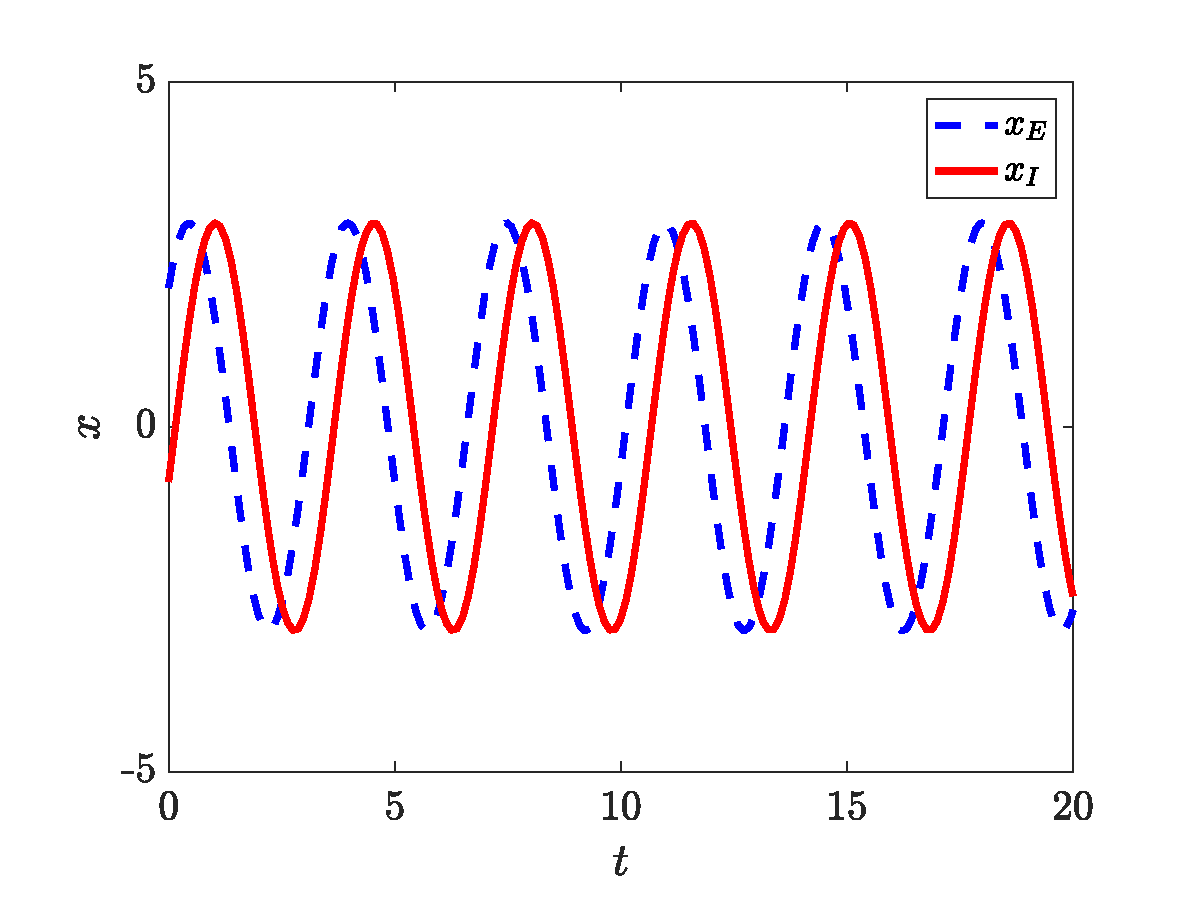
\includegraphics[width=7.8cm]{images/limitcycleIC1.eps}
    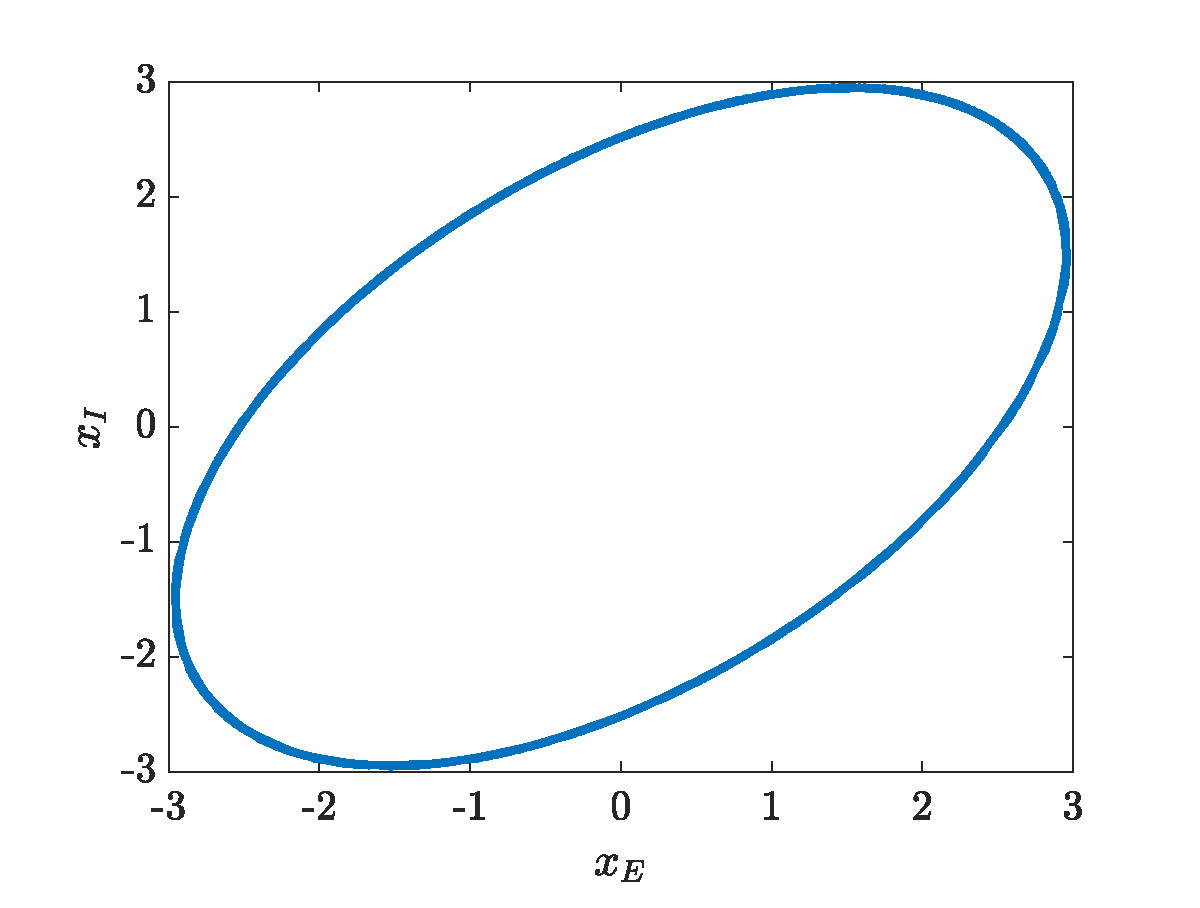
\includegraphics[width=7.8cm]{images/limitcycleIC2.eps}
    \end{tabular}
    \caption{Limit cycle arising from Hopf bifurcation at origin for \cref{eqn:sys_Basic} with inhibitory cell clustering and $\mu_{II} = -\alpha \mu_{EE}$. Left panel shows activity $x_E$ of synchronized excitatory cells and activity $x_I$ of synchronized inhibitory cells vs $t$. Right panel shows $x_I$ vs $x_E$. $N=1600$, $N_{C_I} = 20$, $p_I = 20$,$\alpha = 4$, $\mu_{EE}= 0.7$, $g = 1.02 g_H$. Period of limit cycle is 1.792.} 
    \label{fig:limitcycleIC}
\end{figure}

% We can also choose the weights so that the network is balanced, as in the previous section.
% \begin{align*}
% \mu_{EE} &= \mu && \mu_{IE} = \mu \\
% \mu_{EI} &= -\alpha \mu && \mu_{II} = -\alpha n_{C_I} \mu
% \end{align*}
% In that case, the eigenvalues of $\Hvec$ are
% \begin{itemize}
% \item $\lambda_I := \alpha n_{C_I} \mu > 0$ with multiplicity $(p_I-1) \times n_{C_I} = n_I - n_{C_I}$.
% \item $\lambda_E = -\mu < 0$ with multiplicity $n_E - 1$
% \item $\lambda_{C_I} = -(p_I-1) \alpha n_{C_I} \mu < 0$, with multiplicity $n_{C_I} -1$.
% \item A complex conjugate pair of eigenvalues $\lambda_0 \pm i \omega_0$, with 
% \begin{align*}
%     \lambda_0 &:= \frac{1}{2}\mu(\alpha n_{C_I} - 1)
%       \\
%     \omega_0 &:= \frac{1}{2}\mu \sqrt{ \alpha n_{C_I}+1} \sqrt{\alpha n_{C_I}(4p_I - 1) - 1}
% \end{align*}
% \end{itemize}
% HERE, $\lambda_I$ WILL CROSS BEFORE $\lambda_0$ SO MIGHT GET MORE INTERESTING BEHAVIOR.

\section{Discussion}
In this paper, we analyze a family of clustered excitatory-inhibitory neural networks; and in particular, the underlying bifurcation structures that arise because of permutation symmetries in the network. 

For the simplest case (all-to-all connected, except for self-connections), we extend our results from [REFERENCE HERE]. We show that:
\begin{itemize}
    \item The origin becomes unstable in a symmetric pitchfork bifurcation at $g=g_0$, at which a new branch of solutions emerges for each possible division of the inhibitory cells into two synchronized clusters (the $I_1/I_2$ branch).
    \item Along each such solution branch, a Hopf bifurcation creates a branch of periodic orbits.
    \item All such periodic orbit branches rejoin at a symmetric pitchfork bifurcation of limit cycles, at some large value of the bifurcation parameter $g=g^*$; for $g>g^*$, there is a single stable limit cycle for which the excitatory population and inhibitory population are each synchronized.
\end{itemize}
These basic outlines were present in [REFERENCE]. We extend these results with the following:
\begin{itemize}
    \item An approximate formula for the solution branch $I_1/I_2$ and for the location of the corresponding Hopf bifurcation. ($g_{H,\beta}$, where $\beta = n_{I_1}/n_{I_2}$).
    \item A proof that near $g_0$, the $I_1/I_2$ solution branch is stable for $1\leq \beta < 2$, but unstable otherwise ($\beta \ge 2$).
    \item All $I_1/I_2$ solution branches are unstable for large $g$.
    \item Stability of limit cycles?
\end{itemize}

We next consider the case where the excitatory cells are broken into clusters. The E-E weights are normalized so that the network is still approximated balanced. We find that:
\begin{itemize}
\item The origin becomes unstable at $g=g_C$: for $g>g_C$ there is a branch of solutions corresponding to each possible division of the \emph{excitatory clusters} into synchronized groups (the $C_1/C_2$ branch): we characterize each branch by the ratio of clusters in each group: $\beta_C = n_{C_1}/n_{C_2}$.
\item Near $g_C$, each solution branch is stable for  $1 \le \beta_C < 2$, unstable otherwise.
\item Along each such branch there is a further bifurcation, in which the inhibitory cells split into two clusters.
\item There are no Hopf bifurcations along these branches.
\item For large $g$, the only branches that remain stable are those for which $\beta_C$ is close to $\beta$, in the precise sense we describe in (SAY WHERE HERE); i.e. the excitatory clusters and the inhibitory cells must break up in a similar way.
\end{itemize}

Finally, we consider a network in which the inhibitory cells are clustered, rather than the excitatory cells. Here we find that the origin loses stability in a Hopf bifurcation. 
\begin{itemize}
    \item In contrast to the all-to-all case, the frequency does not increase with $N$.
\end{itemize}

\appendix

\section{Solutions along $I_1/I_2$ branches: detailed calculations} 
Here we derive leading order expressions for the equilibria along the $I_1/I_2$ branches for $g$ close to $g_0$. 

We begin with the simplest case which is when $n_I$ is even and $\beta = 1$. 
Taking $x_{I_1} = x_I$, $x_{I_2} = -x_I$, and $x_E = 0$ in \cref{eq:reducedsystem} and simplifying, we obtain the single equation (\cite[{Eq. 16}]{Barreiro2017})
\[
-x_I + \frac{\alpha \mu_{EE} }{\sqrt{N}} \tanh(g x_I) = 0, 
\]
which simplifies to 
\begin{equation}\label{eq:xIbrancheq}
\tanh(g x_I) - g_0 x_I = 0.
\end{equation}
Defining $f(x_I) := \tanh(g x_I) - g_0 x_I$, $f(0) = 0$, $f'(0) = g - g_0$, and $f(x_I) \rightarrow -\infty$ as $x_I \rightarrow \infty$. When $g > g_0$, $f(x_I)$ is initially increasing, thus it follows from the continuity of $f$ and the intermediate value theorem that \cref{eq:xIbrancheq} has a solution with $x_I > 0$ for all $g > g_0$. Furthermore, $x_I \rightarrow 1/g_0$ as $g \rightarrow \infty$.

To obtain an approximation of this solution for $g$ close to $g_0$, we expand the LHS of \cref{eq:xIbrancheq} in Taylor series about $x_I = 0$ and $g = g_0$ and simplify to get
\begin{equation}\label{eq:tanhTaylor}
(g-g_0) x_I - \frac{(g x_I)^3}{3} + \frac{2(g x_I)^5}{15} + \mathcal{O}\left( x_I^7 \right) = 0.
\end{equation}
We note that the remainder term in $(g-g_0)$ is transcendentally small in the sense of \cite{Holmes2012}. Keeping up to cubic terms in $x_I$, equation \cref{eq:tanhTaylor} simplifies to
\[
x_I \left( (g - g_0) - \frac{g^3}{3} x_I^2 \right) = 0.
\]
Solving for the non-zero solution for $x_I$ results in the expression \cref{eq:xIapprox}.

We can obtain a higher-order approximation by keeping up to fifth-order terms in \cref{eq:tanhTaylor} to get
\begin{equation*}
x_I \left( (g - g_0) - \frac{g^3}{3} x_I^2 + \frac{2 g^5}{15} x_I^4 \right) = 0,
\end{equation*}
which is $x_I$ multiplied by a quadratic in $x_I^2$. To find the nonzero solution for $x_I$, we solve this quadratic for $x_I^2$ and take square roots, yielding \cref{eq:xIapprox5}.

For $\beta > 1$, we find the solution along each $I_1/I_2$ branch by reducing \cref{eq:reducedsystem} to the 3-dimensional system
\begin{equation}\label{eq:otherbranchmatrixeq}
 \begin{aligned}
 \begin{bmatrix} x_E\\x_{I_1}\\x_{I_2}\end{bmatrix} 
 &= \frac{\mu_{EE}}{\sqrt{N}} 
 \begin{bmatrix} (\alpha n_I - 1) & -\alpha \frac{\beta}{\beta+1} n_I & - \alpha \frac{1}{\beta+1} n_I  \\
    \alpha n_I  & -\alpha \left(\frac{\beta}{\beta+1} n_I-1\right) & - \alpha \frac{1}{\beta+1} n_I  \\
    \alpha n_I & -\alpha \frac{\beta}{\beta+1} n_I & -\alpha \left(\frac{1}{\beta+1} n_I-1\right)
 \end{bmatrix}
 \begin{bmatrix} \tanh(g x_E) \\\tanh ( g x_{I_1} ) \\\tanh(g x_{I_2})\end{bmatrix},
 \end{aligned}
 \end{equation}
 where $x_E$ is the activity of the synchronized excitatory cells, $x_{I_1}$ and $x_{I_2}$ are the activities of the two synchronized inhibitory clusters, and we used $n_E = \alpha n_I$. For any solution $(x_E, x_{I_1}, x_{I_2})^T$ to \cref{eq:otherbranchmatrixeq}, $\xvec = (x_E, x_{I_1}, \dots, x_{I_1}, x_{I_2}, \dots, x_{I_2})^T$ is an equilibrium solution to \cref{eq:reducedsystem}, where $x_{I_1}$ and $x_{I_2}$ are repeated $n_{I_1}$ and $n_{I_2}$ times, respectively. As $N \rightarrow \infty$, numerical continuation with the parameter continuation software package AUTO \cite{AUTO} suggests that \cref{eq:otherbranchmatrixeq} has a solution of the form
\begin{equation}\label{eq:I1I2asymp}
    x_{I_2} = -\beta x_{I_1} + \mathcal{O}\left( \frac{1}{N^2} \right), \quad 
    x_{I_1} = \mathcal{O}\left( \frac{1}{N} \right), \quad
     x_E = \mathcal{O}\left( \frac{1}{N^2} \right)
\end{equation}
for $g$ close to $g_0$. Subtracting the second and third equations in \cref{eq:otherbranchmatrixeq}, we get
\[
 x_{I_1} - x_{I_2} = \frac{\alpha}{\mu_{EE}\sqrt{N}}\left( \tanh(g x_{I_1}) - \tanh(g x_{I_2}) \right).
 \]
Substituting \cref{eq:I1I2asymp} as an ansatz, expanding the $\tanh$ terms in a Taylor series about $x_{I_1} = 0$ to cubic order, and simplifying, we obtain the formula given in \cref{eq:XI1}.

\section{Stability and bifurcations along \texorpdfstring{$I_1/I_2$}{I1/I2} branches: detailed calculations}

To determine the stability of $\xvec^*$ for $g$ close to $g_0$, we start by computing the eigenvalues of $D\tilde{F}(\xvec^*)$ corresponding to $\lambda_{I_1}$ and $\lambda_{I_2}$. Substituting \cref{eq:XI1} for $x_{I_1}$, using the Taylor series expansion $\sech^2 x = 1 - x^2 + \mathcal{O}(x^4)$, and simplifying, the eigenvalue $\lambda_{I_1}^*(g)$ of $D\tilde{F}(\xvec^*)$ is located at
\begin{align*}
    \lambda_{I_1}^*(g) &= \frac{g-g_0}{g} \left( 1 - \frac{3}{1-\beta+\beta^2 }\right) + \mathcal{O}\left(\frac{1}{N^2} \right) && g > g_0,
\end{align*}
which is negative for $1 \leq \beta < 2$ and positive for $\beta > 2$. Similarly, the eigenvalue $\lambda_{I_2}^*(g)$ of $D\tilde{F}(\xvec^*)$ corresponding to $\lambda_{I_2}$ is located at 
\begin{align*}
    \lambda_{I_2}^*(g) &= \frac{g-g_0}{g} \left( 1 - \frac{3 \beta^2}{1-\beta+\beta^2 }\right) + \mathcal{O}\left(\frac{1}{N^2} \right) && g > g_0,
\end{align*}
which is negative for $\beta > 1/2$ and thus does not affect stability. 


It remains to find leading order expressions for the eigenvalues of $H_3(\xvec)$. When $\xvec = 0$, the matrix $H_3(0)$ has a single eigenvalue at $\lambda_I$ and a complex conjugate pair of eigenvalues $\lambda_0 \pm \omega_0$, where these are defined at the beginning of this section. These do not depend on $\beta$. For $\xvec$ small but nonzero, we use a perturbation method to approximate the eigenvalues of $H_3(\xvec)$. We substitute the expressions \cref{eq:I1I2asymp} into characteristic polynomial for $H_3(\xvec)$, keeping only terms of up to order $1/N$ so that the leading order expression only involves $x_{I_1}$. We then use the Taylor expansion $\sech^2(g x_{I_1}) = 1 - (g x_{I_1})^2 + \mathcal{O}( x_{I_1}^4 )$, keeping only terms up to quadratic order. For each eigenvalue $\lambda$ of $H_3(\xvec)$, we use a power series ansatz 
\begin{equation}\label{eq:lambdaansatz}
\lambda + \epsilon x_{I_1}^2 + \mathcal{O}(x_{I_1})^4.
\end{equation}
We substitute this ansatz into the characteristic polynomial for $H_3(\xvec)$ and solve for $\epsilon$ by matching the coefficients of $x_{I_1}^2$. (This computation, and the remaining computations in this section, were performed with the aid of Wolfram Mathematica). Using this method for $\lambda = \lambda_I$, $H_3(\xvec^*)$ has a real eigenvalue located at
\[
\lambda_I(\xvec^*) = \alpha \mu_{EE} \left(1 - (1-\beta+\beta^2)g^2 x_{I_1}^2 \right) + \mathcal{O}\left(\frac{1}{N^2} \right).
\]
Substituting the estimate \cref{eq:XI1} for $x_{I_1}$ and simplifying, the eigenvalue $\lambda_I^*(g)$ of $J_3(\xvec)$ corresponding to $\lambda_I$ is located at
\begin{align*}
\lambda_I^*(g) = \frac{\alpha \mu_{EE} g}{\sqrt{N}} \left( 1 - \frac{3(g-g_0)}{g}\right) - 1 &= -2\left( \frac{g - g_0}{g_0} \right) + \mathcal{O}\left(\frac{1}{N^2} \right) && g \geq g_0,
\end{align*}
which is always negative and thus does not affect stability.

Finally, we use this method to locate the eigenvalue of $H_3(\xvec)$ corresponding to $\lambda_0 \pm \omega_0$. In doing so, we will find a Hopf bifurcation on each $I_1/I_2$ branch. $H_3(\xvec)$ has a complex conjugate pair of eigenvalues, where the real part is given by
\begin{equation}
\lambda_0(g, \beta) = \frac{\mu_{EE}}{2}\left( \alpha - 1 + \alpha \beta g^2 (n_I-1) x_{I_1}^2 \right) + \mathcal{O}\left(\frac{1}{N} \right).
\end{equation}
We can get more accurate approximations for $\lambda(g, \beta)$ by taking higher powers of $x_{I_1}$ in our power series ansatz \cref{eq:lambdaansatz}. For example, when $\beta=1$, we can obtain the fourth-order approximation
\[
\lambda_0(g, 1) = \frac{\mu_{EE}}{2}\left( \alpha - 1 + \alpha g^2 (n_I-1) x_{I_1}^2 - \frac{2}{3}\alpha g^4 (n_I-1) x_{I_1}^4 \right) + \mathcal{O}\left(\frac{1}{N^2} \right).
\]
A similar fourth-order approximation can be obtained when $\beta>1$, but the resulting coefficient of $x_{I_1}^4$ is extremely complicated.
Substituting \cref{eq:XI1} for $x_{I_1}$ and simplifying, $J_3(\xvec)$ has a complex conjugate pair of eigenvalues $\lambda_0^*(g) \pm i \omega_0^*(g)$, where
\begin{equation}\label{eq:lambdagbeta}
\lambda_0^*(g, \beta) = \frac{\mu_{EE} g}{2 \sqrt{N}}\left[ \alpha - 1 + \alpha \beta (n_I-1) \frac{ 3(g - g_0) }{ (1 - \beta + \beta^2 )g} \right] - 1 + \mathcal{O}\left(\frac{1}{N} \right).
\end{equation}
To locate the Hopf bifurcation on each $I_1/I_2$ branch, which occurs when the complex pair of eigenvalues crosses the imaginary axis, we solve $\lambda_0^*(g, \beta) = 0$ for $g$, substitute $g_0 = \sqrt{N}/\alpha \mu_{EE}$, and simplify to obtain the expression in \cref{eq:ghopfformula}.


\section{Proof of \cref{prop:limitcycle}}\label{sec:limitcycleproof}

The $\beta = \infty$ limit cycle is a periodic solution to the two-dimensional system
\begin{equation}\label{eq:2dimsystem}
\begin{aligned}
\dot{x_1} &= f_1(x_1, x_2) := -x_1 + \frac{\mu_{EE}}{\sqrt{N}}\left((n_E - 1) \tanh(g x_1) - \alpha n_I \tanh(g x_2) \right) \\
\dot{x_2} &= f_2(x_1, x_2) := -x_2 + \frac{\mu_{EE}}{\sqrt{N}}\left( n_E \tanh(g x_1) - \alpha (n_I - 1) \tanh(g x_2) \right), 
\end{aligned}
\end{equation}
where $x_1$ represents the synchronized excitatory cell activity and $x_2$ represents the synchronized inhibitory cell activity. First, we show that that \cref{eq:2dimsystem} has no fixed points other than the origin. To do this, we make the change of variables $(y_1, y_2) = (\tanh(g x_1),\tanh(g x_2))$, and note that it is equivalent to show that the system of equations
\begin{equation}\label{eq:2dimsystemy}
\begin{aligned}
g_1(y_1, y_2) := -\frac{1}{g}\tanh^{-1}(y_1) + \frac{\mu_{EE}}{\sqrt{N}}\left((n_E - 1) y_1 - \alpha n_I y_2 \right) = 0 \\
g_2(y_1, y_2) := -\frac{1}{g}\tanh^{-1}(y_2) + \frac{\mu_{EE}}{\sqrt{N}}\left( n_E y_1 - \alpha (n_I - 1) y_2 \right) = 0
\end{aligned}
\end{equation}
has no solution other than $(y_1, y_2) = (0,0)$. The first equation $g_1(y_1, y_2) = 0$ is satisfied when
\begin{equation}\label{eq:y2sol}
y_2 = y_2^*(y_1) := \frac{ g \mu_{EE} (n_E-1) y_1 - \sqrt{N} \tanh^{-1}(y_1)}{\alpha g \mu_{EE} n_I}.
\end{equation}
To show that \cref{eq:2dimsystemy} has no solutions other than the origin, we substitute \cref{eq:y2sol} into $g_2(y_1, y_2)$ to get 
\begin{equation}
\begin{aligned}
g_2(y_1, y_2^*(y_1)) &= \frac{\mu_{EE}( n_E + n_I - 1) y_1 }{n_I \sqrt{N}} + \frac{n_I - 1}{g n_I} \tanh^{-1}(y_1) \\
&\qquad+ \frac{1}{g} \tanh^{-1} \left( \frac{ \sqrt{N} \tanh^{-1}(y_1) - g \mu_{EE}(n_E -1) y_1}{ \alpha g \mu_{EE} n_I } \right).
\end{aligned}
\end{equation}    
We will show that $g_2(y_1, y_2^*(y_1)) > 0$ for $y_1 > 0$. Since $g_2(y_1, y_2^*(y_1))$ is an odd function in $y_1$, this will imply that $g_2(y_1, y_2^*(y_1)) < 0$ for $y_1 < 0$, from which the desired result will follow. Since $\tanh^{-1}y_1 \geq y_1$ for $y_1 \geq 0$, it suffices to show that
\begin{equation}\label{eq:h}
\begin{aligned}
h(y_1) &:= \frac{\mu_{EE}( n_E + n_I - 1) y_1 }{n_I \sqrt{N}} + \frac{n_I - 1}{g n_I} \tanh^{-1}(y_1) \\
&\qquad+ \frac{1}{g} \tanh^{-1} \left( \frac{ \sqrt{N} \tanh^{-1}(y_1) - g \mu_{EE}(n_E -1) y_1}{ \alpha g \mu_{EE} n_I } \right) > 0
\end{aligned}
\end{equation}
for $y_1 > 0$. Since $h(0) = 0$, we will show that $h'(0) > 0$ for $y_1 > 0$. Computing the derivative with the assistance of Mathematica,
\begin{equation*}\label{eq:hprime}
\begin{aligned}
h'(y_1) &= 
\frac{(N-1)\mu_{EE}}{(1-f) N^{3/2} } + \frac{1}{g(1 - y_1^2)} 
- \frac{
 f \mu_{EE} N ( g \mu_{EE} ( f N - 1) - \sqrt{N}}{f^2 g^2 \mu_{EE}^2 N^2 - (\sqrt{N} + 
 g \mu_{EE}(1 - f N))^2 y_1^2} \\
 &\geq \frac{(N-1)\mu_{EE}}{(1-f) N^{3/2} } + \frac{1}{g(1 - y_1^2)} 
- \frac{1}{g \left( 1 - \left( \frac{ f N - 1}{f N} \right)^2 y_1^2 \right)} \\
&\geq \frac{(N-1)\mu_{EE}}{(1-f) N^{3/2} } > 0.
\end{aligned}
\end{equation*}
We have therefore shown that \cref{eq:2dimsystem} has no fixed points other than the origin.

The Linearization of \cref{eq:2dsystem} about the origin is the $2 \times 2$ matrix
\[
J = \frac{g \mu_{EE}}{\sqrt{N}}
\begin{bmatrix} 
n_E - 1 & -\alpha n_I \\
n_E & -\alpha(n_I - 1)
\end{bmatrix} - I_2,
\]
which has a complex conjugate pair of eigenvalues $\frac{g}{\sqrt{N}}(\lambda_0 \pm i \omega_0) - 1$, where $\lambda_0$ and $\omega_0$ are defined in \cref{sec:E1I1}. It follows that the origin is repelling for $g > g_H$, which is the Hopf bifurcation point \cref{eq:0hopflocation}. To show there is a limit cycle for $g > g_H$, we use the Poincar{\'e}-Bendixson theorem \cite[Chapter 16]{Coddington1955}. For a trapping region, we draw a square around the origin with corners $(-a, -a)$ and $(a, a)$. On the line $x = a$, for $a$ large,
\[
\dot{x} \leq -a + \frac{2 n_E}{\sqrt{N}} = -a + 2 f \sqrt{N},
\]
which can be made negative by taking $a$ sufficiently large. Similarly, we can take $a$ sufficiently large so that the vector field defined \cref{eq:2dsystem} points inward at all points on the square (\cref{fig:nullclines}). Since the origin is repelling for $g > g_H$ and is the only fixed point of the system, it follows from the Poincar{\'e}-Bendixson theorem that there is a limit cycle surrounding the origin for $g > g_H$. We note that although the limit cycle from \cref{prop:limitcycle} is stable in the two-dimensional system \cref{eq:2dsystem}, the theorem says nothing about its stability in the full system \cref{eqn:sys_Basic}.
\begin{figure}
    \centering
    \begin{tabular}{c}
    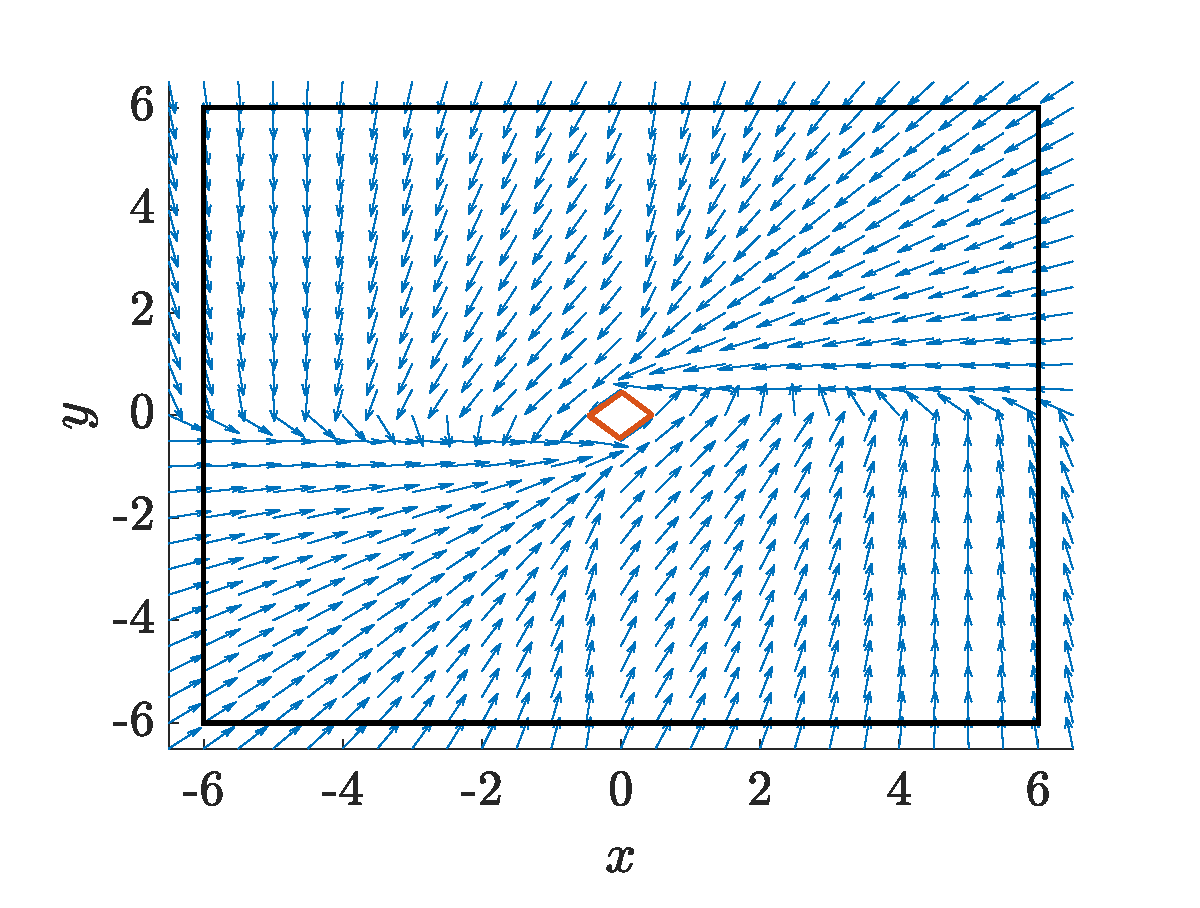
\includegraphics[width=8cm]{images/trappingregion.eps}
    \end{tabular}
    \caption{Slope fields for \cref{eq:2dsystem}, with a small limit cycle visible in center. Slope field points inward on black box, which is the trapping region for the Poincar{\'e}-Bendixson theorem. $N = 20$, $g = 5$, $\alpha = 4$, and $\mu_{EE} = 0.7$.}
    \label{fig:nullclines}
\end{figure}

\bibliographystyle{siamplain}
\bibliography{main.bib}

\end{document}
